\RequirePackage{silence} % :-\
    \WarningFilter{scrbook}{Usage of package `titlesec'}
    \WarningFilter{hyperref}{Composite letter}
    \WarningFilter{titlesec}{Non standard sectioning command detected}
\documentclass[11pt,paper=a4,footinclude=true,headinclude=true]{scrbook} % KOMA-Script book
\usepackage[T1]{fontenc}
\usepackage[slovene]{babel}
\usepackage{xspace}
\usepackage[  linedheaders=false,%
              parts=true]{classicthesis} % ,manychapters
%\usepackage[osf]{libertine}
\usepackage{xcolor}

\definecolor{codegreen}{rgb}{0,0.6,0}
\definecolor{codegray}{rgb}{0.5,0.5,0.5}
\definecolor{codepurple}{rgb}{0.58,0,0.82}
\definecolor{backcolour}{rgb}{0.95,0.95,0.92}

\usepackage{listings}
\usepackage{xpatch}
\usepackage{realboxes}

\lstdefinestyle{mystyle}{
    backgroundcolor=\color{backcolour},   
    commentstyle=\color{codegreen},
    keywordstyle=\color{magenta},
    numberstyle=\tiny\color{codegray},
    stringstyle=\color{codepurple},
    %basicstyle=\footnotesize,
    basicstyle=\ttfamily,
    breakatwhitespace=false,         
    breaklines=true,                 
    captionpos=b,                    
    keepspaces=true,                 
    numbers=left,                    
    numbersep=5pt,                  
    showspaces=false,                
    showstringspaces=false,
    showtabs=false,                  
    tabsize=2,
    language=Caml, 
}
\lstset{style=mystyle}

\makeatletter
\xpretocmd\lstinline{\Colorbox{backcolour}\bgroup\appto\lst@DeInit{\egroup}}{}{}
\makeatother

\usepackage{hyperref}
\usepackage{amssymb,amsmath,amsthm}
\usepackage{answers}
\usepackage{enumitem}

%\newcounter{moncompteur}
\theoremstyle{definition}
\newtheorem{ex}{%
	\hyperlink{ex:\theex}{Vaja}\hypertarget{sol:\theex}{}}[chapter]
\Newassociation{sol}{Odgovor}{ans}
\renewenvironment{Odgovor}[1]
{\par\bigskip\noindent{\bfseries \hypertarget{ex:#1}{}\hyperlink{Sol:#1}{Re\v sitev za vajo #1:}}\quad}
{\par\bigskip}

%\Newassociation{sol}{Odgovor}{ans}
%\newtheorem{ex}{Vaja}[chapter]
\usepackage{mathtools} % Bonus

\newcommand{\myTitle}{Koncepti programskih jezikov\xspace}
\newcommand{\mySubtitle}{Vaje za predmet Programiranje II\xspace}
\newcommand{\myName}{Matja\v z Krnc, Iztok Savnik\xspace}
\newcommand{\myAuthors}{Iztok Savnik, Matja\v z Krnc\xspace}
\newcommand{\shortAuthors}{I. Savnik, M. Krnc\xspace}
\newcommand{\myStudents}{...\xspace}
\newcommand{\myProf}{Put name here\xspace}
\newcommand{\myOtherProf}{Put name here\xspace}
\newcommand{\mySupervisor}{Put name here\xspace}
\newcommand{\myFaculty}{Fakulteta za matematiko, naravoslovje in informacijske tehnologije\xspace}
\newcommand{\myDepartment}{DIST\xspace}
\newcommand{\myUni}{Univerza na Primorskem\xspace}
\newcommand{\myLocation}{Koper\xspace}
\newcommand{\myYear}{2018\xspace}
\newcommand{\myMonth}{December\xspace}
\newcommand{\myISBN}{978-961-288-966-1\xspace}
\newcommand{\myCOBISSID}{297674496\xspace}
\renewcommand{\myVersion}{2.}
\renewcommand{\myStudents}{
Andra\v z Cuderman,
Davor Fon,
Mateja Gri\v zon,
Nejc Razpotnik,
Neja Sko\v cir}
%\newcommand{\textcopyright}{This work is licensed under a Creative Commons Attribution 3.0 Unported License</a>\xspace}

% document 
\begin{document}
	%*******************************************************
% Titlepage
%*******************************************************
\begin{titlepage}
    % if you want the titlepage to be centered, uncomment and fine-tune the line below (KOMA classes environment)
    \begin{addmargin}[-1cm]{-3cm}
    \begin{center}
        \large

        \hfill

        \vfill

        \begingroup
            \color{Maroon}\spacedallcaps{\myTitle} \\ \bigskip
        \endgroup

        \spacedlowsmallcaps{\myAuthors}

        \vfill

        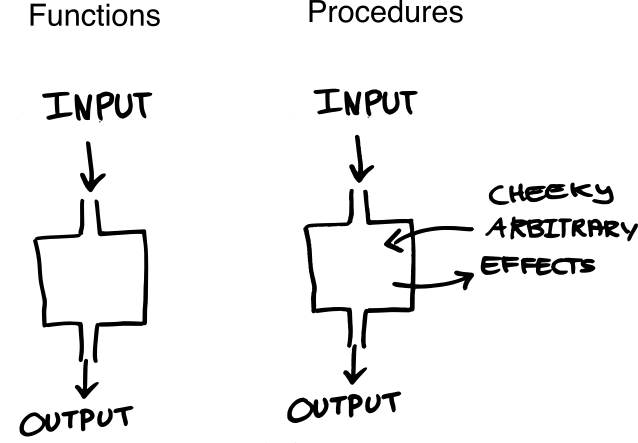
\includegraphics[width=6cm]{ext/frontpage.png} \\ %\medskip %11 cm when A4
		\vfill %
        \mySubtitle \\ %\medskip
        \vfill %
        %\myDegree \\
        %\myDepartment \\
        %\myFaculty \\
        %\myUni \\ \bigskip
		%\vfill%
        \myMonth, \myYear\ -- Verzija \myVersion

        \vfill

    \end{center}
  \end{addmargin}
\end{titlepage}

    \begin{addmargin}[-4cm]{-1cm}
	{	\setlength{\fboxsep}{6mm}
	\noindent\fbox{
	\begin{minipage}[b][1.8cm][c]{11cm} % velikost okvira skatle je 11 cm x 6,5 cm
	\small
	CIP -- Katalo\v zni zapis o publikaciji\\
	Narodna in univerzitetna knji\v znica, Ljubljana
	\vfill
	ISBN \myISBN  (pdf)\\
	COBISS.SI-ID=\myCOBISSID
	\end{minipage}
	}}
	
\vspace*{\fill}
\noindent
\thispagestyle{empty}
\begin{tabular}{ll}
%Lektorirala: ...\\[3mm]
\multicolumn{2}{ l }{\textbf{\myTitle}} \\
\multicolumn{2}{ l }{\emph{\mySubtitle}} \\[6mm]
%\textbf{Urednika:} & \myName\\[3mm]
\textbf{Avtorja:} & \parbox[t]{6cm}{\myAuthors \vspace{3mm}}\\
\textbf{Samozalo\v zba in oblikovanje:} & Matja\v z Krnc\\[3mm]
%E-posta: knjiga@vidra.net\\[3mm]
%Za zalozbo: Andrej Klemenc\\[3mm]
%\textbf{Oblikovanje:} & Matjaž Krnc\\[3mm]
\textbf{Fotografija na naslovnici:} & \parbox[t]{6cm}{FPComplete Blog \vspace{3mm}}\\
%\textbf{ISBN:} &  \myISBN \\
%\textbf{COBISS-ID:} &  \myCOBISSID \\
\textbf{Na\v cin dostopa (URL):} &  \href{http://bit.ly/KPJ-vaje}{\texttt{bit.ly/KPJ-vaje}} \\[3mm]
%Priprava za tisk: \\[3mm]
%Tisk: \\[3mm]
\myLocation, \myMonth \myYear
\end{tabular}


\end{addmargin}
    %\vspace*{\fill}
\noindent
\thispagestyle{empty}
\begin{tabular}{ll}
%Lektorirala: ...\\[3mm]
\multicolumn{2}{ l }{\textbf{\myTitle}} \\
\multicolumn{2}{ l }{\emph{\mySubtitle}} \\[6mm]
%\textbf{Urednika:} & \myName\\[3mm]
\textbf{Avtorja:} & \parbox[t]{6cm}{\myAuthors \vspace{3mm}}\\
\textbf{Samozalo\v zba in oblikovanje:} & Matja\v z Krnc\\[3mm]
%E-posta: knjiga@vidra.net\\[3mm]
%Za zalozbo: Andrej Klemenc\\[3mm]
%\textbf{Oblikovanje:} & Matjaž Krnc\\[3mm]
%\textbf{Fotografija na naslovnici:} & \parbox[t]{6cm}{\emph{Durer graph} by Koko90 - Own work. Licensed under CC BY-SA 3.0 \vspace{3mm}}\\
\textbf{ISBN:} &  \myISBN \\
%Priprava za tisk: \\[3mm]
%Tisk: \\[3mm]
\myLocation, \myMonth \myYear
\end{tabular}
\clearpage


\endinput
    \chapter{Uvod}

\noindent
Zakaj u\v cenje konceptov programskih jezikov? \\
Posplo\v sevanje abstrakcij podanih v konkretnih jezikih \\
Novi predmeti na podro\v cju programskih jezikov \\
%``Multipardigm'' programski jeziki Scala, C#, F#, ... \\

\noindent
Osnovna ideja strukture zbirke? \\
Prva klasifikacija podro\v cij so modeli programskih jezikov \\
Znotraj modelov so pomembni koncepti \\
\v student naj bi preko nalog ponovil/obnovil poznavanje posameznih konceptov \\

\noindent
Osnovne ideje predstavitve podro\v cja \\
U\v citi se ve\v cih PJ? \\
\v sola programskih jezikov bli\v zje teoriji programskih jezikov \\
Pri predstavitvi smo bli\v zje matemati\v cni, logi\v cni razlagi \\
U\v cenje o abstrakcijah in o implentaciji PJ \\

\noindent
Zakaj OCaml? \\
Meta Language ML, trenutni trendi v na\v crtovanju jezikov \\ 
Osnova \v cisti lambda ra\v cun \\
OCaml pokriva \v stiri razli\v cne modele \\

\noindent
Kak\v sne vrste nalog imamo?
Temeljni/klasi\v cni problemi iz danegih modelov programskih jezikov \\
Primer, imperativni jeziki, delo s polji \\
Matemati\v cni problemi, blizu teorije programskih jezikov \\

\noindent
Re\v sitve so podane v OCaml \\
Lahko uporabimo tudi primeren jezik iz danega modela jezikov? \\




    %%\begin{addmargin}[-1cm]{-1cm}
	{\vspace*{\fill}
	\setlength{\fboxsep}{6mm}
	\noindent\fbox{
	\begin{minipage}[b][6.5cm][c]{11cm} % velikost okvira skatle je 11 cm
							% x 6,5 cm
	\small
	CIP -- Katalo\v zni zapis o publikaciji\\
	Narodna in univerzitetna knji\v znica, Ljubljana
	
	\vfill

	xxx.x(xxx)(x.xxx.x)
	\vfill

	DISKRETNA matematika [Elektronski vir] : / avtorji 
	\shortAuthors ; [urednika] \myName. - \verzija.  - El. knjiga. - Ljubljana : samozal. \myYear.
	\vfill
	
	Način dostopa (URL): \url{http://www.xxxxxxxxxxxxxx.xx}
	
	\vfill
	
	ISBN \myISBN  (pdf)\\
	1. xxxxxt, xxxxx 2. xxxx, xxxxxx 
	286126336
	\vfill
	
	\end{minipage}}}
%\end{addmargin}
\endinput
    \tableofcontents

%   \automark[section]{chapter}
%   \renewcommand{\chaptermark}[1]{\markboth{\spacedlowsmallcaps{#1}}{\spacedlowsmallcaps{#1}}}
%   \renewcommand{\sectionmark}[1]{\markright{\thesection\enspace\spacedlowsmallcaps{#1}}}

    % use \cleardoublepage here to avoid problems with pdfbookmark
    \cleardoublepage
    \part{Vaje}\label{part:testpart}
    \Opensolutionfile{ans}[ans1]
	%from functional to ...
%classes in oopl
%act records to imperative

\chapter{Uvod}

Zakaj učenje konceptov programskih jezikov? \\
Posploševanje abstrakcij podanih v konkretnih jezikih \\
Novi predmeti na področju programskih jezikov \\
%``Multipardigm'' programski jeziki Scala, C#, F#, ... \\

Osnovna ideja strukture zbirke? \\
Prva klasifikacija področij so modeli programskih jezikov \\
Znotraj modelov so pomembni koncepti \\
Študent naj bi preko nalog ponovil/obnovil poznavanje posameznih konceptov \\

Osnovne ideje predstavitve področja \\
Učiti se večih PJ? \\
Šola programskih jezikov bližje teoriji programskih jezikov \\
Pri predstavitvi smo bližje matematični, logični razlagi \\
Učenje o abstrakcijah in o implentaciji PJ \\

Zakaj OCaml? \\
Meta Language ML, trenutni trendi v načrtovanju jezikov \\ 
Osnova čisti lambda račun \\
OCaml pokriva štiri različne modele \\

Kakšne vrste nalog imamo?
Temeljni/klasični problemi iz danegih modelov programskih jezikov \\
Primer, imperativni jeziki, delo s polji \\
Matematični problemi, blizu teorije programskih jezikov \\

Rešitve so podane v OCaml \\
Lahko uporabimo tudi primeren jezik iz danega modela jezikov? \\



\chapter{Lambda ra\v cun}


\begin{ex}
Napi\v si izraz v lambda ra\v cunu, ki za dana parametra x in y izra\v cuna povpre\v cno vrednost x in y.

Apliciraj prej definiran lambda izraz na konkretnih parametrih in zapi\v si redukcijo izraza do vrednosti.
\end{ex}




\begin{ex}
Uporabi alfa konverzijo in beta redukcijo za ovrednotenje naslednjega stavka zapisanega z $\lambda$-ra\v cunom
$$(\lambda a.\lambda b.a (a b)) (\lambda a.a + 1)\,1.$$

a) Izra\v cunaj vrednost izraza.

b) Kaj naredi funkcija?
\end{ex}




\begin{ex}
Evaluiraj naslednje lambda izraze do vrednosti.

1) $( \lambda f.f( \lambda x.x))( \lambda x.x) $

2) $( \lambda x. \lambda y.x) z w$

\end{ex}



\begin{ex}
Dane imamo naslednje standardne kombinatorje lambda ra\v cuna.
\begin{align*}
I& \equiv \lambda x.x;\\
K& \equiv \lambda x.\lambda y.x;\\
K^*& \equiv \lambda x.\lambda y.y;\\
S& \equiv \lambda x. \lambda y.\lambda z.xz(yz)
\end{align*}
Poenostavi naslednje izraze:
\begin{align*}
M &\equiv (\lambda x.\lambda y.\lambda z.zyx)aa(\lambda p.\lambda q.q);\\
M &\equiv (\lambda y.\lambda z.zy)((\lambda x.xxx)(\lambda x.xxx))(\lambda w.I);\\
M &\equiv SKSKSK
\end{align*}
\end{ex}



\begin{ex}
V naslednjih $\lambda$-izrazih prika\v zi vse oklepaje.  
\begin{itemize}
\item $(\lambda x.xa)ax$ 
\item $(\lambda z.zxz)(\lambda y.yx)z$ 
\end{itemize}
\end{ex}




\begin{ex}
Poi\v s\v ci vse proste (nevezane) spremenljivke v naslednjih $\lambda$-izrazih. 
\begin{itemize}
\item $(\lambda b.xba)xb$ 
\item $\lambda x.zy\lambda y.yx $
\end{itemize}
\end{ex}



\begin{ex}
Napi\v si naslednji izraz z \v cim manj oklepajev. 

 \begin{itemize}
 \item $((xy)(\lambda y.(\lambda z.(z(\lambda y.(xy)))x)y)) $
 \end{itemize}
\end{ex} 



\chapter{Funkcijski programski jeziki}


\section{Matemati\v cne funkcije}



\begin{ex}
Napi\v si funkcijo v ML, ki izra\v cuna vsoto vrste: 
$$1+4+9+16+...+n^2.$$

\begin{sol}
\begin{lstlisting}
function n -> n * (n + 1) * (2*n + 1)/6
\end{lstlisting}
\end{sol}

\end{ex}



\begin{ex}
Napi\v si funkcijo v ML, ki izra\v cuna vsoto vrste 
$$\sum_{x=0}^n 1/(2^x) = 1/1+1/2+1/4+1/8+1/16+...+1/(2^n).$$

Preveri delovanje funkcije z implementacijo v Ocaml.
\begin{sol}
\begin{lstlisting}
    
let rec vsota_vrste n = match n with
| 1 -> 1.
| _ -> 1./.2.**(float_of_int n) +. (vsota_vrste (n-1))
\end{lstlisting}
\end{sol}
\end{ex}



\begin{ex}
V Ocaml napi\v si funkcijo, ki izra\v cuna n-to Fibonaccijevo \v stevilo definirano na slede\v c na\v cin:
\begin{center}
$F_n = 1$, \v ce $n\in \left\{ 0,1\right\}$, ter 
$F_n$ = $F_{n-1} + F_{n-2}$, 
\end{center}
pri \v cemer zapis $F_i$ predstavlja i-to Fibonaccijevo \v stevilo. 

Fibonaccijevo zaporedje: 1, 1, 2, 3, 5, 8, 13, 21, 34, 55, 89, 144, 233, ...

\begin{sol}
\begin{lstlisting}
let rec fib n = match n with
| 0 -> 1
| 1 -> 1
| _ -> fib (n-2) + fib (n-1);;
\end{lstlisting}
\end{sol}
\end{ex}



\begin{ex}
Dana je OCaml funkcija naslednik (\lstinline{let naslednik n = n+1}). Z uporabo funkcije naslednik in brez uporabe artimeti\v cnih operacij naredi funkcijo \lstinline{jeVsota(a:int, b:int, c:int)}, ki preveri ali je c vsota a in b (pri \v cemer velja $a,b\geq 0$).


\begin{sol}
\begin{lstlisting}
let rec jeVsota (a, b, c) = match b with
| 0 -> if (a = c) then true
else false
| b -> jeVsota ((naslednjik a), b-1, c)
\end{lstlisting}
\end{sol}



\end{ex}
\begin{ex}
Funkcija \lstinline{pfib: int*int -> int*int} je definirana na slede\v c na\v cin:
$$
\mathtt{pfib}(i,j)=\begin{cases}
(1,1); & i,j\le0;\\
\mathtt{pfib}(i-1,0); & j=0;\\
\mathtt{pfib}(0,j-1); & i=0;\\
\mathtt{pfib}(i-1,j-1)+\mathtt{pfib}(i-2,j-2); & else.
\end{cases}
$$
Operacija '+' je definirana nad pari na obi\v cajen na\v cin. Definiraj funkcijo \lstinline{pfib} v Ocaml.

\begin{sol}
\begin{lstlisting}
let vsota (a,b)(c,d) = (a+c, b+d)

let rec pfib (a,b) = match (a,b) with
| (i, j) when i <= 0 && j<=0 -> (1,1)
| (i, 0) -> pfib (i-1, 0)
| (0, j) -> pfib (0, j-1)
| (i, j) -> vsota (pfib (i-1, j-1)) (pfib (i-2, j-2))    
\end{lstlisting}
\end{sol}



\end{ex}
\begin{ex}
\emph{Ackermannova funkcija} je definirana z rekurzivnimi ena\v cbami.
\begin{align*}
A(0, n) &= n+1 \\
A(m + 1, 0) &= A(m, 1) \\ 
A(m + 1, n + 1) &= A(m, A(m + 1, n)) 
\end{align*}

Napi\v si funkcijo \lstinline{A : int -> int -> int}, ki izra\v cuna za dana parametra $m$ in $n$ vrednost zgoraj definirane rekurzivne funkcije.
\end{ex}




\begin{ex}
Dana je funkcija se\v stej : a' list -> int, ki se\v steje elemente danega seznama.

\begin{lstlisting}
# let rec sestej l = match l with
 | [] -> 0
 | a::r -> a+sestej r;; 
val sestej : int list -> int = <fun> 
# sestej [1;2;3];; 
- : int = 6 

\end{lstlisting}
Predstavi vsa stanja aktivacijskih zapisov ob klicu funkcije sestej [1;2;3].

\begin{sol}
\begin{lstlisting}
sestej [1;2;3] = 1+ sestej [2;3]
sestej [2;3] = 2+ sestej[1]
sestej[1] = 1+ sestej []
sestej[] = 0
sestej[1] = 1+ 0=1
sestej [2;3] = 2+ 1=3
sestej [1;2;3] = 1+ 3=4
\end{lstlisting}
\end{sol}
\end{ex}



\section{Seznami}


\begin{ex}
Napi\v si funkcijo sestej: \lstinline{int list -> int}, ki se\v steje elemente celo\v stevilskega seznama.

Primer: 
\begin{lstlisting}
# sestej [1;2;3;4;5];;
- : int = 15 
\end{lstlisting}

\begin{sol}
\begin{lstlisting}
let rec sestej sez = match sez with
| []->0
| hd::tl -> hd+(sestej tl)
\end{lstlisting}
\end{sol}



\end{ex}
\begin{ex}
Napi\v si funkcijo \lstinline{unija : int list -> int list -> int list}, ki za dana seznama celih \v stevil vrne unijo. Pazi na duplikate!

Primer: \begin{lstlisting} 
# unija [1;2;4;7] [2;4;7;9];; 
- : int list = [1;2;4;7;9]
\end{lstlisting}

\begin{sol}
\begin{lstlisting}
let rec najdi e = function
| [] -> false
| h::t ->if( h == e) then true else najdi e t

let rec unija l1 l2 =
match l1 with
| [] -> l2
| h::t -> if najdi h l2 then unija t l2
else unija t (h::l2)
\end{lstlisting}
\end{sol}



\end{ex}
\begin{ex}
Napi\v si funkcijo \lstinline{zdruzi : int list -> int list -> int list}, ki sprejeme urejena seznama kot parametra in vrne urejen seznam, ki vsebuje elemente obeh vhodnih seznamov.

Primer: \begin{lstlisting}
# zdruzi [2;3;4] [5;7;9;10;13];;
- : int list = [2;3;4;5;7;9;10;13]
\end{lstlisting}

\begin{sol}
\begin{lstlisting}
let zdruzi sez1 sez2 = sez1 @sez2

(* ali *)

let rec zdruzi sez1 sez2 = match (sez1, sez2) with
| ([], s) -> s
| (t, []) -> t
| (a::b, c::d) -> if a<=c then [a]@ (zdruzi b (c::d))
else [c]@(zdruzi (a::b) d)
\end{lstlisting}
\end{sol}



\end{ex}
\begin{ex}
Napi\v si funkcijo \lstinline{zdruzi : int list -> int list -> int list}, ki zdru\v zi dva seznama v tretji seznam tako, da vzame najprej en element iz prvega seznama potem dva elementa iz drugega seznama in tako naprej dokler ne pride do konca enega izmed vhodnih seznamov. Preostanek nepraznega seznama se da na konec novega seznama.

Primer: \begin{lstlisting}
# zdruzi [1;2;3] [5;6;7;8];;
- : int list = [1;5;6;2;7;8;3]
\end{lstlisting}

\begin{sol}
\begin{lstlisting}
et rec zdruzi (sez1,sez2) = match (sez1,sez2) with
| ([],x) -> x 
| (x,[]) -> x 
| (g1::[],g2::r2) -> g1::g2::r2 
| (g1::r1,g2::[]) -> g1::g2::r1 
| (g1::r1,g2::g22::r2) -> g1::g2::g22:: zdruzi (r1,r2);;
\end{lstlisting}
\end{sol}
\end{ex}



\begin{ex}
Napi\v si funkcijo \lstinline{vecjeod : int list -> int -> int list}, ki dobi seznam in \v stevilo, vrne pa seznam, ki vsebuje samo elemente ve\v cje od podanega \v stevila.

Primer: \begin{lstlisting}
# vecjeod [2;5;26;87;2;6]  5;;
- : int list = [26;87;6] 
\end{lstlisting}

\begin{sol}
\begin{lstlisting}
let rec vecjeod sez n = match sez with
| []->[]
| hd::tl -> if(hd>n) then hd::(vecjeod tl n) else (vecjeod tl n)
\end{lstlisting}
\end{sol}

\end{ex}



\begin{ex}
Napi\v site funkcijo \lstinline{seznamnm : int -> int list}, ki izpi\v se seznam \v stevil od \v stevila n do m. Velja $n\le m$.

Primer: \begin{lstlisting}
# seznamnm 5 11;;
- : int list = [5;6;7;8;9;10;11] 
\end{lstlisting}

\begin{sol}
\begin{lstlisting}
let rec seznamnm n m =
if n > m then []
else n :: seznamnm (n+1) m;;
\end{lstlisting}
\end{sol}



\end{ex}
\begin{ex}
Napi\v si funkcijo \lstinline{palindrom: int list -> bool}, ki preveri, \v ce je podan seznam celih \v stevil palindrom.

Primer: \begin{lstlisting}
# palindrom [1;2;3;2;1];;
- : bool = true
# palindrom [1;2;3];;
- : bool = false
\end{lstlisting}

\begin{sol}
\begin{lstlisting}
let palindrom sez =
sez = List.rev sez
\end{lstlisting}
\end{sol}

\end{ex}



\begin{ex}
Napi\v si funkcijo \lstinline{vsotaSodeLihe: int list -> int*int}, ki za dani seznam posebej se\v steje soda in liha \v stevila, ter vrne par, ki ima na prvem polo\v zaju vsoto lihih \v stevil, na drugem pa vsoto sodih \v stevil.

Primer: \begin{lstlisting}
# vsotaSodeLihe [1;1;1;2;4];;
- : int*int = (3,6)
\end{lstlisting}

\begin{sol}
\begin{lstlisting}
let rec vsotaSodeLihe sez = match sez with
| [] -> (0, 0)
| a::b -> let (l,s) = vsotaSodeLihe b in 
if (a mod 2 = 1) then 
(l+a, s) 
else 
(l, s+a)
\end{lstlisting}
\end{sol}



\end{ex}
\begin{ex}
Napi\v si funkcijo \lstinline{podseznam : int list -> int list -> bool}, ki preveri ali je seznam podan kot prvi parameter podseznam seznama podanega kot drugi parameter funkcije.

Primer: \begin{lstlisting}
# podseznam [1;2] [3;4;1;2];;
- : bool = true
# podseznam [1;2] [1;2;3];;
- : bool = true
# podseznam [1;2] [4;2];;
- : bool = false
\end{lstlisting}

\begin{sol}
\begin{lstlisting}
let rec podseznam sez1 sez2 = match (sez1, sez2) with
| ([], _) -> true
| (a::b, c::d) when List.length sez1 <= List.length sez2 -> if (a=c) then podseznam b d else false
| _ -> false
\end{lstlisting}
\end{sol}



\end{ex}
\begin{ex}
  Dan imamo seznam znakov tipa \lstinline{char list} v katerem se lahko
  pojavijo samo znaka \lstinline{'a'} in \lstinline{'b'}. Napi\v si funkcijo
  \lstinline{cnta : char list -> int list}, ki pretvori sekvence znakov v
  seznam celih \v stevil po naslednjih pravilih:

    -- \lstinline{aaa -> 3},
    
    -- \lstinline{aa -> 2},
    
    -- \lstinline{a -> 1} in
    
    -- \lstinline{x -> 0}, kjer je \lstinline{x} poljuben znak.

\noindent\/Primer:
\begin{lstlisting}
# cnta ['a','a','a','a','a','b','a','a'];;
- : int list = [3,2,0,2]
\end{lstlisting}

\begin{sol}
\begin{lstlisting}
let rec cnta sez = match sez with
| [] -> []
| 'a'::'a'::'a'::r -> 3 :: cnta r 
| 'a'::'a'::r -> 2 :: cnta r 
| 'a'::r -> 1 :: cnta r 
| _::r -> 0 :: cnta r;;
\end{lstlisting}
\end{sol}
\end{ex} 



\begin{ex}
Funkcijo za sortiranje seznama implementiraj na slede\v c na\v cin:

\begin{enumerate}
\item Napi\v si pomo\v zno funkcijo zamenjaj : \lstinline{int list -> int list}, ki poi\v s\v ce v seznamu prvi zaporeden par \lstinline{...::x::y::rep}, ki ni pravilno urejen: $x>y$. Funkcija naj vrne par sestavljen iz 
	\begin{enumerate}
	\item istega seznama, kjer sta x in y zamenjana ter 
    \item true v primeru, da je bila zamenjava narejena in false sicer.
	\end{enumerate}
    \item Napisi funkcijo \lstinline{sortiraj : int list -> int list}, ki ponavlja izvajanje funkcije zamenjaj tako dolgo dokler ni seznam urejen.
\end{enumerate}
\end{ex}
\begin{ex}
Dan je seznam, ki vsebuje znake tipa char. Napi\v si funkcijo \lstinline{ace}, ki sprejme seznam znakov in vrne true v primeru, da seznam znakov vsebuje znake seznama ['a';'c';'e'] v danem vrstnem redu in false sicer. 

\begin{lstlisting}
# ace ['a';'b';'r';'a';'k';'a';'d';'a';'b';'r';'a'];;
- : bool = false
# ace ['a';'b';'e';'c';'e';'d';'a'];;
- : bool = true
# ace ['c';'e';'d';'r';'a'];;
- : bool = false
\end{lstlisting}

\begin{sol}
\begin{lstlisting}
let rec ace1 sez count = match sez with
| [] -> false
| a::b -> if (count = 0 && a = 'a') then ace1 b 1
else if(count = 1 && a = 'c') then ace1 b 2
else if (count = 2 && a = 'e') then true
else ace1 b count

let ace sez = ace1 sez 0
\end{lstlisting}
\end{sol}

\end{ex}



\begin{ex}
Dan je seznam, ki vsebuje vrednosti 0 in 1. Napi\v si funkcijo, ki naredi naslednjo transformacijo na seznamu. Vse pojavitve vzorca 111 zamenja z vrednostjo 3, vse pojavitve vzorca 11 z vrednostjo 2 ter ohrani samostojne enice 1 in ni\v cle 0. 
\begin{lstlisting}
1 1 1 -> 3
1 1 -> 2
1 -> 1
0 -> 0
\end{lstlisting}

Funkcija vedno posku\v sa najprej zamenjati dalj\v si niz enic.

Na primer, seznam \lstinline{[1;1;0;1;1;1;1;1;0;1;0]} se pretvori v seznam \lstinline{[2;0;3;2;0;1;0]}.

\begin{sol}
\begin{lstlisting}
let rec fja list = match list with
| [] -> []
| a::[] -> [a]
| a::b when a=0 -> a::(fja b)
| a::b::c when a=1 && b=0 ->[a; b]@(fja c)
| a::b::c when a=1 && b=1 && c=[] -> [2]@(fja c)
| a::b::c::d when a=1 && b=1 -> if c=1 then [3]@(fja d)
else [2; c]@(fja d)
\end{lstlisting}
\end{sol}
\end{ex}



\begin{ex}
  Napi\v si funkcijo cikli : int -> int -> int, ki za klic cikli m n
  generira seznam n ciklov \v stevil od 0 do m-1.

\noindent\/Primer:
\begin{lstlisting}
# cikli 3 4;; 
- : int list = [0; 1; 2; 0; 1; 2; 0; 1; 2; 0; 1; 2]
\end{lstlisting}

\begin{sol}
\begin{lstlisting}
let rec stevila n m = let x=m-1 in
if n > x then []
else n :: stevila (n+1) m;;

let rec cikli m n = match n with
| 0 -> []
| _ -> (stevila 0 m)@cikli m (n-1)
\end{lstlisting}
\end{sol}

\end{ex} 



%----
\begin{ex}
  \label{dnk-naloga}
  Dano imamo sekvenco DNK v obliki seznama znakov tipa \lstinline{dnk list},
  kjer je tip \lstinline{dnk} definiran kot

  \begin{lstlisting}
  type dnk = A | C | T | G
  \end{lstlisting}
  Na primer, niz znakov "ACAAGT"  je predstavljen s seznamom 
  \lstinline{[A;\-C;A;A;G;T]}. 

  Napi\v si funkcijo \lstinline{najpodniz : dnk list -> int*int}, ki
  poi\v s\v ce najdalj\v si podniz istih znakov tipa \lstinline{dnk} ter
  izpi\v se pozicijo prvega znaka in dol\v zino niza.
\end{ex} 



\begin{ex}
  Dano imamo sekvenco DNK v obliki seznama znakov tipa \lstinline{dnk list},
  kjer je tip \lstinline{dnk} definiran kot v Nalogi \ref{dnk-naloga}.

  Napi\v si funkcijo \lstinline{prestej : dnk list -> dnk*int list}, ki
  se\v steje enake zaporedne znake v sekvenci in za vsako skupino
  kreira par, ki vsebuje \lstinline{dnk} znak in \v stevilo pojavitev
  znaka.

  \emph{Primer}: 
  \begin{lstlisting}
  # prestej [A;C;A;A;G;C;C];;
  val - : dnk*int list = [(A,1);(C,1);(A,2);(G,1);(C,2)]
  \end{lstlisting}
\end{ex} 



\begin{ex}
  Napi\v si funkcijo \lstinline{zamenjaj : int list -> int list}, ki v
  enem prehodu poi\v s\v ce v seznamu celih \v stevil vse zaporedne
  pare \lstinline{x::y}, ki niso urejeni po nara\v s\v cajo\v cem vrstnem
  redu (\lstinline{x<=y}) in jih obrne.

  Z uporabo funkcije \lstinline{zamenjaj} implementiraj sortiranje seznama.
\end{ex} 



\begin{ex}
  Relacijo $\mathcal{R}$ predstavimo s seznamom parov celih \v
  stevil. Napi\v si funkcijo

  \begin{lstlisting}
  razsiri : int*int list -> int list -> int list,
  \end{lstlisting}

  kjer je prvi parameter seznam parov \lstinline{r} in drugi parameter
  seznam celih \v stevil \lstinline{s}. Rezultat funkcije
  \lstinline{razsiri} naj bo seznam, ki vsebuje vsa \v stevila \lstinline{x}
  za katera velja \lstinline{(e,x)}$\in\mathcal{R}$ za nek element e
  seznama \lstinline{s}.
\end{ex} 



\begin{ex}
  Napi\v si funkcijo

  \begin{lstlisting}
  zdruzi : int list -> int list -> int list,
\end{lstlisting}

  ki zdru\v zi urejena seznama celih \v stevil tako, da je rezultat
  urejen in hkrati izlo\v ci ve\v ckratne ponovite elementov.

  \begin{sol}
  \begin{lstlisting}
  let rec zdruzi list1 list2 = match (list1, list2) with
  | ([], []) -> []
  | (a, []) -> a
  | ([], b) -> b
  | (a::b, c::d) -> 
       if (a < c ) then a::(zdruzi b (c::d))
       else if (c<a) then c::(zdruzi (a::b) d)
            else a::(zdruzi b d)
  \end{lstlisting}
  \end{sol}
\end{ex} 



\begin{ex}
  Dana je funkcija \lstinline{fib3}, ki je definirana na slede\v c na\v cin:
\begin{lstlisting}
  fib3(n) = 1, za n=1,2,3
  fib3(n) = fib3(n-1)+fib3(n-2)+fib3(n-3), za n>3.
\end{lstlisting}

  Napi\v si funkcijo 
  \lstinline{fib3list : int -> int list}, ki generira seznam
  vrednosti funkcije fib3 od $1$ do $n$, kjer je $n>0$ parameter funkcije.

\noindent\/Primer:
\begin{lstlisting}
# fib3 6;;
_ : int list = [1; 1; 1; 3; 5; 9]
\end{lstlisting}

%\begin{sol}
%\begin{lstlisting}
%let rec fib3 x = match x with
%| 0 -> []
%| _ -> match fib3(x-1) with
%| [] -> [1]
%|	[_] -> [1;1]
%| [;] -> [1;1;1]
%|	a::b::c::_ as smallfib -> (a+b+c)::smallfib;;
%
%let rec obrni sez = match sez with
%| [] -> []
%| g::r -> (obrni r)@[g];;
%
%obrni (fib3 6);;
%
%note: not optimal. feel free to edit. I'm not planing on doing HM with this
%\end{lstlisting}
%\end{sol}
\end{ex} 



\begin{ex}
Napi\v si funkcijo v Ocaml, ki za dani seznam celih \v stevil se\v steje soda in liha \v stevila, ter vrne par, ki ima na prvem mestu vsoto lihih \v stevil, na drugem pa vsoto sodih \v stevil.

\end{ex} 



\begin{ex}
  Seznam tipa (string*string) list predstavlja lete neke letalske
  dru\v zbe. Vsak par opi\v se direkten let med dvemi mesti. Napi\v si
  funkcijo

\begin{lstlisting}
povezava : (string*string) -> (string*string) list -> bool,
\end{lstlisting}

  ki preveri ali obstaja povezava med dvemi mesti podanimi s prvim
  parametrom. Povezava je lahko direktna ali z enim vmesnim
  postankom. Seznam letov letalske dru\v zbe je podan z drugim
  parametrom. Funkcija vrne true v primeru, da povezava obstaja in
  false sicer.

  Dodatne to\v cke: Naj povezava pomeni poljubno povezavo, ki je
  sestavljena iz poljubnega \v stevila vmesnih postankov.
\end{ex} 



\begin{ex}Naloga je sestavljena iz dveh delov.

  a) Definiraj tip plist, ki predstavi seznam parov. Prva komponenta
  para vsebuje klju\v ce tipa int in druga komponenta vrednosti tipa
  string.

  b) Napi\v si funkcijo  
\begin{lstlisting}
vapply : plist -> (string -> string) -> plist,
\end{lstlisting}
  ki aplicira funkcijo tipa \lstinline{string -> string} (drugi parameter) na vseh
  drugih komponentah parov, ki so podani s prvim parametrom
  funkcije. 

  Rezultat naj bo seznam parov kjer je druga komponenta vhodnih parov
  zamenjana z vrednostjo funkcije 
  \lstinline{string -> string}.
\end{ex} 




\section{Polimorfizem}



\begin{ex}
Napi\v si polimorfi\v cno funkcijo 

\begin{center}
\lstinline{zdruzi : 'a list -> 'a list -> ('a*'a->'a) -> 'a list}, 
\end{center}

ki zdruzi dva enako dolga seznama poljubnih objektov, tako da zdru\v zi istole\v zne objekte seznamov. Par istole\v znih objektov seznamov zdru\v zimo z uporabo tretjega parametra funkcije zdruzi, funkcijo tipa \lstinline{'a*'a->'a}.

Napi\v si primer uporabe funkcije zdruzi nad seznamoma celih \v stevil. Zdru\v zitev dveh \v stevil implementiraj z obi\v cajno vsoto. 
\end{ex}



\begin{ex}
  Napi\v si polimorfi\v cno funkcijo
  \begin{lstlisting}
  ostevilci : 'a list -> (int * 'a) list, 
  \end{lstlisting}
  ki o\v stevil\v ci elemente od $1$ do $n$, \v ce je n dol\v zina
  vhodnega seznama. Funkcija ostevilci naj vrne seznam parov, kjer je
  prva komponenta indeks in druga komponenta orginalna vrednost iz
  seznama.
\end{ex} 



\begin{ex}
Tip ('a*'b) list opisuje seznam parov kjer je prva komponenta klju\v c tipa 'a in druga komponenta vrednost tipa 'b. 

Napi\v si funkcijo 

meet : ('a*'b) list -> ('a*'b) list -> ('a*('b*'b)) list,

ki zdru\v zi dva seznama sortirana po klju\v cu tipa 'a. Pari iz vhodnih seznamov se zdru\v zijo samo v primeru, da se ujemajo v klju\v cu. Rezultat funkcije so pari sestavljeni iz klju\v ca in vrednosti, ki vsebuje obe vrednosti iz vhodnih parov.  

Primer:    
\begin{lstlisting}
meet [(1,2);(2,3);(4,5);(4,9)] [(2,4);(4,6)] -> 
     [(2,(3,4));(4,(5,6));(4,(9,6))]
\end{lstlisting}
\end{ex} 



\begin{ex}
  Tip ('a*'b) list opisuje seznam parov, kjer je prva komponenta para
  klju\v c tipa 'a in druga komponenta vrednost tipa 'b.

  Predpostavimo, da so vhodni seznami sortirani po klju\v cu tipa
  'a. Napi\v si funkcijo

\begin{lstlisting}
diff : ('a*'b) list -> ('a*'b) list -> ('a*'b) list,
\end{lstlisting}

  ki izra\v cuna razliko dveh seznamov. Rezultat vsebuje vse pare iz
  prvega seznama s klju\v ci, ki se ne pojavijo v drugem seznamu.

\noindent\/Primer:    
\begin{lstlisting}
diff [(1,2);(2,3);(4,5)];(5,6)] [(2,4);(4,6)] -> [(1,2);(5,6)]
\end{lstlisting}



\end{ex} 
\begin{ex}
Napi\v si parametri\v cno funkcijo 
\begin{lstlisting}
podseznam : 'a list -> int*int -> 'a list, 
\end{lstlisting}
ki iz danega seznama izlu\v s\v ci podseznam dolo\v cen z drugim parametrom funkcije $(z,k)$, 
kjer $z$ predstavlja indeks za\v cetka podseznama in $k$ indeks konca podseznama. 

Predpostavimo, da je $z<k$ in $k<l$, kjer je $l$ dol\v zina vhodnega seznama. 
\end{ex} 



\begin{ex}
  Dan je seznam parov, ki vsebujejo klju\v c tipa 'k in vrednost tipa
  'v. Napi\v si funkcijo
\begin{lstlisting}
  filter ('v->bool) -> 'k*'v list -> 'k list,
\end{lstlisting}
  ki iz seznama parov dolo\v cenim z 2. parametrom izbere tiste klu\v
  ce za katere vrne funkcija \lstinline{('v->bool)} dolo\v cena s 1. parameterom
  vrednost true. Rezultat funcije filter je seznam tak\v snih klju\v
  cev.

\noindent\/Primer:
\begin{lstlisting}
# filter (function x -> x=0) [(1,0);(2,1);(3,0);(4,1)];; 
- : int list = [1; 3] 

\end{lstlisting}
\end{ex} 



\section{Funkcije vi\v sjega reda}



\begin{ex}
Napi\v si funkcijo vi\v sjega reda 
\begin{center}
\lstinline{urediPar : 'a*'a -> ('a*'a->bool) -> 'a*'a}, 
\end{center}
ki za dan par vrednosti tipa 'a*'a vrne isti par vrednosti urejen po velikosti. Za dolo\v citev vrstnega reda komponent para napi\v si funkcijo 
\lstinline{vecji : 'a*'a -> bool}, 
ki vrne \lstinline{true}, \v ce je prva komponenta ve\v cja od druge. Uporabi funkcijo ve\v cji kot parameter funkcije \lstinline{urediPar}.

\end{ex}
\begin{ex}
Napi\v si funkcijo vi\v sjega reda 
\begin{center}
\lstinline{izberi l f: 'a list -> ('a -> bool) -> 'a list},
\end{center}
ki iz seznama l izbere samo
tiste elemente a za katere funkcija f vrne true.
Primer: 
\begin{lstlisting}
# let f a = if a>2 then true else false;;
val f : int -> bool = <fun>
# izberi [1;2;3;5] f;;
- : int list = [3; 5]
\end{lstlisting}
\end{ex}



%----
\begin{ex}
  Napi\v si funkcijo vi\v sjega reda

  \begin{lstlisting}
  skrci : (int * int -> int) -> list int -> int,
  \end{lstlisting}
  katere prvi parameter \lstinline{f : int*int -> int} je funkcija, ki
  zdru\v zi dve vrednost iz seznama v en samo vrednost tipa
  \lstinline{int}. Drugi parameter \lstinline{skrci} je seznam celih \v
  stevil.

  Naj bo funkcija \lstinline{f} prvi parameter in seznam \lstinline{l = [i1; i2; ...; in] } drugi parameter. Pomen funkcije \lstinline{skrci}
  lahko zapi\v semo na naslednji na\v cin.

  \begin{lstlisting}
  skrci f l = f i1 (f i2 f(...(f in-1 in)))
  \end{lstlisting}
  Predpostavi, da ima seznam \lstinline{l} vsaj dva elementa!
\end{ex}



\begin{ex}
Napi\v si funkcijo vi\v sjega reda 

\begin{lstlisting}
foldx : 'a list -> 'b -> ('a -> 'b -> 'b) list -> 'b,
\end{lstlisting}
ki nad seznamom, ki je podan s prvim argumentom, in za\v cetno vrednostjo podano z drugim argumentom, aplicira funkcije iz seznama podanega kot tretji argument na slede\v c na\v cin. 

Naj bo prvi argument enak \lstinline{[a1,a2,...,an]},
drugi argument \lstinline{b}, in tretji argument enak
\lstinline{[f1,f2,...,fn]}. 
Rezultat dobimo na slede\v c na\v cin: 
\begin{lstlisting}
    f1 a1  (f2 a2 ... (fn  an b) ...)
\end{lstlisting}


\end{ex} 

%\section{Implementacija funkcij} <-- merged with matematicne funkcije





\section{Rekurzivni tipi}
%Rekurzivni tipi?





\begin{ex}
Dan imamo seznam, definiran z rekurzivnim podatkovnim tipom izraz. 
\begin{lstlisting}
type izraz = 
      Nil 
    | Stevilo of int * izraz 
    | Oper of char * izraz ;; 
\end{lstlisting}
Izraz vsebuje aritmeti\v cne izraze, ki so lahko sestavljeni iz \v stevil (Stevilo) in operacij (Oper). Dovoljene operacije so plus '+' in minus '-'. Predpostavljamo, da izrazi opisujejo pravilne aritmeti\v cne izraze.

Napi\v si funkcijo ovrednoti : izraz -> int, ki izra\v cuna vrednost izraza.
Primer: 
\begin{lstlisting} 
    e = 10 + 5 - 3
\end{lstlisting}

\end{ex}






\begin{ex}
  Binarno drevo je definirano s tipom
\begin{lstlisting}
type bdrevo = List of int |
            Drevo of bdrevo * int * bdrevo,
\end{lstlisting}
  ki ima vrednosti v listih definirane kot \lstinline{List v}, kjer je
  $v$ celo \v stevilo.  Notranja vozli\v s\v ca so definirana kot
  trojica \lstinline{Drevo (l, v, d)}, kjer sta $l$ in $d$ levo in desno
  poddrevo, $v$ pa je vrednost%, ki je za\v cetno $0$ za vsa notranja vozli\v s\v ca.
.
  \begin{enumerate}[label=(\roman*)]
  \item Napi\v si funkcijo \lstinline{prestej : bdrevo -> int}, 
    ki vrne vsoto vrednosti podanih v listih vhodnega drevesa.

  \item Napi\v si funkcijo
    \lstinline{oznaci : bdrevo -> bdrevo,}
    ki drugo komponento vseh notranjih vozli\v s\v c izhodnega drevesa
    zamenja z vsoto vseh listov poddrevesa.
  \end{enumerate}
\begin{sol}
Naloga (i):
\begin{lstlisting}
let rec prestej dr = match dr with
| List x -> x
| Drevo (a,b,c) -> prestej a + prestej c
\end{lstlisting}
Naloga (ii):
\begin{lstlisting}
let rec oznaci dr = match dr with
| List a -> dr 
| Drevo (d,f,g) -> Drevo (oznaci d, prestej dr ,oznaci g)
\end{lstlisting}
\end{sol}
\end{ex}




\begin{ex}
  Binarno drevo je definirano s tipom itree, ki predstavlja binarno
  drevo katerega vozli\v s\v ca vsebujejo vrednost tipa int.
\begin{lstlisting}
  type itree = Nil | Node of itree*int*itree;;
\end{lstlisting}

  Napi\v si funkcijo sumsub : itree -> itree, ki iz vhodnega drevesa
  konstruira novo drevo, ki namesto originalnih vrednosti v voli\v s\v
  cih vsebuje vsoto vrednosti vozli\v s\v c levega in desnega
  pod-drevesa ter vrednosti danega vozli\v s\v ca.

\noindent\/Primer:
\begin{lstlisting}
# sumsub Node(Node(Nil,3,Nil),5,Node(Nil,2,Node(Nil,1,Nil)));;
_ : itree = Node(Node(Nil,3,Nil),11,Node(Nil,3,Node(Nil,1,Nil)))
\end{lstlisting}
\end{ex} 




\begin{ex}
Dan je tip bdrevo, ki je definiran na naslednji na\v cin

\begin{lstlisting}
type bdrevo = Leaf of int | Node of bdrevo * int * bdrevo;;
\end{lstlisting}

Napi\v si funkcijo bapply : bdrevo -> (int -> int) -> bdrevo, ki aplicira funkcijo (int -> int) na vseh vozli\v s\v cih drevesa.  
\end{ex} 





\begin{ex}
Drevo je definirano z naslednjim tipom. 

\begin{lstlisting}
type bindrevo = List of int | Drevo of bindrevo * bindrevo ;; 
\end{lstlisting}

Napi\v si funkcijo izpis : bindrevo -> int -> unit, ki izpi\v se vse liste katerih vrednost je ve\v cja od drugega parametra. 
\end{ex} 





\begin{ex}
  Drevo int\_tree je definirano na naslednji na\v cin.

\begin{lstlisting}
type int_tree = { mutable key:int; mutable trees: int_tree list}
\end{lstlisting}

  Napi\v si funkcijo vi\v sjega reda

\begin{lstlisting}
tree_filter : int_tree -> int -> int list.
\end{lstlisting}

  Funkcija vrne seznam vseh klju\v cev iz drevesa podanega s prvim
  parametrim, ki so ve\v cji od vrednosti podane z drugim parametrom
  funkcije.
\end{ex} 





\section{Parametrizirani tipi}




%sez
\begin{ex}
Dan imamo seznam, definiran z naslednjim tipom. 
\begin{lstlisting}
type 'a seznam = 
      Nil 
    | Vrednost of 'a * 'a seznam;; 
\end{lstlisting}

Seznam je urejen v nara\v s\v cajo\v cem vrstnem redu glede na vrednost primerjalne funkcije primerjaj : 'a -> 'a -> int , ki vrne -1 \v ce je prvi parameter ve\v cji od drugega, 0 \v ce sta enaka in 1 v primeru, da je drugi parameter ve\v cji od prvega.

Napi\v si parametri\v cno funkcijo:
\begin{lstlisting}
dodaj : 'a seznam -> ('a -> 'a -> int) -> 'a
\end{lstlisting}
kjer je prvi parameter seznam v katerega dodajamo, drugi parameter je funkcija primerjaj in tretji parameter vrednost tipa 'a, ki jo dodajamo v seznam.
\end{ex}




\begin{ex}
  Seznam definiramo z zapisom, ki ima dve komponenti: vrednost tipa
  \lstinline{'a} in kazalec na naslednji element seznama tipa \lstinline{'a seznam}, ki je bodisi prazen ali pa ima še vsaj en element.

  \begin{lstlisting}
  type 'a element = { 
     mutable vrednost:'a; 
     mutable naslednji:'a seznam 
  }
  and 'a seznam = Prazen | Element of 'a element ;;
  \end{lstlisting}

  Napi\v si funkcijo \lstinline{podvoji : 'a seznam -> 'a seznam}, ki
  podvoji vse vrednosti v seznamu.
\end{ex} 




\begin{ex}
  Podatkovna struktura \lstinline{seznam} je definirana na naslednji na\v
  cin.

  \begin{lstlisting}
  type 'a element = { 
     mutable vrednost: 'a; 
     mutable naslednji: 'a seznam 
  }
  and 'a seznam = Prazen | Element of 'a element ;;
  \end{lstlisting}

  Napi\v si funkcijo 
  \lstinline{zdruzi : 'a seznam -> 'a seznam -> 'a seznam}, ki ima za argumenta dva seznama tipa \lstinline{'a seznam}.

  \begin{enumerate}[label=(\roman*)]
  \item Funkcija naj zdru\v zi seznama tako, da pove\v ze konec prvega
    seznama z za\v cetkom drugega ter kot rezultat vrne za\v cetek prvega
    seznama.

  \item Funkcija naj zdru\v zi seznama tako, da naredi kopijo obeh
    seznamov v novem seznamu, ki vsebuje na novo konstruirane
    elemente.
  \end{enumerate}
\end{ex} 




%drev
\begin{ex}
  Dan je tip \lstinline{grm}, ki je definiran na slede\v c na\v cin:

\begin{lstlisting}
type 'a grm = 
    Nic 
  | Ena of 'a * 'a grm 
  | Dva of 'a grm * 'a * 'a grm;;
\end{lstlisting}

  Napi\v si funkcijo \lstinline{dolzinevej : 'a grm -> unit}, ki izpi\v
  se dol\v zine vej grma po principu levo-v-globino.
\end{ex} 




\begin{ex} 
  Podan je tip \lstinline{'a drevo} s katerim je predstavljeno binarno
  drevo.

  \begin{lstlisting}
  type 'a drevo = { 
      mutable levo:'a bin_drevo; 
      mutable vozlisce:'a; 
     mutable desno:'a bin_drevo 
  } 
  and 'a bin_drevo = Prazen | Vozlisce of 'a drevo ;;
  \end{lstlisting}

  Napi\v si funkcijo, ki izpi\v se vsa vozli\v s\v ca tretjega nivoja
  drevesa, ki obstajajo v drevesu.
\end{ex} 




\begin{ex}
Dano je drevo definirano z naslednjo podatkovno strukturo:

\begin{lstlisting}
	# type 'a tree = Empty | Node of 'a * 'a tree list ;;
\end{lstlisting}
Napi\v si funkcijo "prestej : 'a tree -> int" , ki pre\v steje vozli\v s\v ca drevesa.
\end{ex}




\begin{ex}
Dana je definicija parametri\v cnega binarnega drevesa. Parameter tipa bindrevo je spremenljivka tipa 'a, ki predstavlja tip elementov v listih drevesa.

\begin{lstlisting}
	type 'a bindrevo = List of 'a | Drevo of 'a bindrevo * 'a bindrevo ;;
\end{lstlisting}

a) Napi\v si funkcijo izpis: 'a bindrevo -> ('a -> bool) -> unit, ki zpi\v se vse liste drevesa za katere vrne drugi parameter funkcije izpis -- funkcija tipa 'a -> bool -- vrednost true. 

b) Napi\v si funkcijo obrni: 'a bindrevo -> 'a bindrevo, ki obrne vhodno drevo tako, da vsa leva poddrevesa zamenja z desnimi poddrevesi. 

\end{ex}




\begin{ex}
Dano imamo splo\v sno planarno drevo, ki je predstavljeno z naslednjim tipom:

\begin{lstlisting}
	type 'a tree = Empty 
               | Node of 'a * 'a tree list ;; 
\end{lstlisting}
Napi\v si funkcijo 
\lstinline{filter :'a tree -> ('a -> bool) -> 'a tree}, 
ki pome\v ce ven iz drevesa vsa poddrevesa s korenom za katerega vrne funkcija tipa 
\lstinline{'a -> bool},
podana kot drugi parameter, vrednost \lstinline{false}. Rezultat je torej novo drevo brez izbranih poddreves. 
\end{ex}




\begin{ex}
  Dani so tip 'a izraz, ki predstavja aritmeti\v cne izraze nad
  vrednostmi tipa \lstinline{'a}
\begin{lstlisting}
  type operacija = PLUS|MINUS;;
  type 'a izraz = 'a | 'a izraz * operacija * 'a izraz;;
\end{lstlisting}
  ter funkciji 
  \lstinline{plus :'a->'a->'a} in
  \lstinline{minus :'a->'a->'a}, 
  ki izra\v cunata vsoto in
  razliko vrednosti tipa 'a.

  Napi\v si funkcijo izracun : 'a izraz -> 'a, ki izra\v cuna vrednost
  izraza tipa 'a izraz.

\noindent\/Primer:
\begin{lstlisting}
# izracun (2,plus,(3,minus,1));;
- : int = 4
\end{lstlisting} 
\end{ex} 





%old
\begin{ex}
Napi\v si polimorfi\v cno rekurzivno funkcijo obrni: 'a array -> 'a array, ki obrne vsebino polja.

Primer: 
\begin{lstlisting}
# obrni [|1;2;3|];;
- : int array = [| 3; 2; 1 |]
\end{lstlisting}

\begin{sol}
\begin{lstlisting}
let obrni polje = let len=Array.length polje in
for i=0 to (len/2) do 
let temp = polje.(i) in
polje.(i) <- polje.(len-i-1);
polje.(len-i-1) <- temp 
done;
polje;;
\end{lstlisting}
\end{sol}
\end{ex}




\begin{ex}
S poljem \v zelimo implementirati parametri\v cno podatkovno strukturo minvrsta, ki hrani zadnjih n najmanj\v sih vrednosti vstavljenih v podatkovno strukturo. Podatkovno strukturo minvrsta definiramo na slede\v c na\v cin:

\begin{lstlisting}
# type 'a minvrsta = 'a array;; 
type minvrsta = 'a array 
\end{lstlisting}
Z naslednjo funkcijo kreiramo primerek minvrsta.

\begin{lstlisting}
# let kreiraj n v = Array.create n v;;   
val kreiraj : int -> int array = <fun> 
# let a : int minvrsta = kreiraj 10 0;; 
val a : int minvrsta = [|0; 0; 0; 0; 0; 0; 0; 0; 0; 0|] 
\end{lstlisting}
Napi\v si parametri\v cno funkcijo dodaj : 'a -> 'a minvrsta -> unit, ki doda novo vrednost v polje. Paziti je potrebno, da polje vedno vsebuje n najmanj\v sih vrednosti.
\end{ex}




\begin{ex}
Dano je drevo, ki vsebuje dve vrsti elementov. Definirano je z naslednjo podatkovno strukturo:


\begin{lstlisting}
	type ('a,'b) drevo = 
     Prazno 
   | Vozliscea of 'a * ('a,'b) drevo list;;  
   | Vozlisceb of 'b * ('a,'b) drevo list;; 
\end{lstlisting}
Napi\v si funkcijo razcepi : ('a,'b) drevo -> 'a list * 'b list, ki prepi\v se vse elemente Vozliscea v prvi seznam in vse elemente Vozlisceb v drugi seznam.

\begin{sol}
\begin{lstlisting}
let razcepi drevo =
let a = ref[] in
let b = ref[] in
let rec raz dr = match dr with
| Prazno ->(!a,!b)
| Vozliscea(x,y) -> a := !a @ [x]; raz y
| Vozlisceb(x,y) -> b := !b @ [x]; raz y
in
raz drevo;;
\end{lstlisting}
\end{sol}
\end{ex}




\begin{ex}
Naloga je sestavljena iz dveh delov:
\begin{enumerate}
    \item Definiraj parametri\v cno podatkovno strukturo 'a splosnoDrevo, kjer spremenljivka tipa 'a predstavlja tip vrednosti vozli\v s\v ca. Splo\v sno drevo ima poljubno \v stevilo poddreves. 
    
    \item Napi\v si funkcijo prestejOtroke : 'a splosnoDrevo -> int, ki izra\v cuna povpre\v cno \v stevilo otrok za vsa vozli\v s\v ca, ki niso listi drevesa.
\end{enumerate}

\end{ex}




%----- nekateg.
\begin{ex}
  Definiraj parametriziran tip \lstinline{'a seznam} z uporabo zapisov!
  Zapis naj ima dve komponenti: vrednost tipa \lstinline{'a} in kazalec na
  naslednji zapis v seznamu oz. prazen seznam.

  Napi\v si funkcijo \lstinline{dolzina : 'a seznam -> int}, ki
  pre\v steje \v stevilo vrednosti v seznamu.
\end{ex} 




\begin{ex}
Definiraj parametri\v cni tip \lstinline{slika}, ki predstavlja dvo dimenzionalno ra\v cunalni\v sko sliko z neznanim tipom elementov (pik) polja, ki ga ozna\v cimo z \lstinline{'a}.

Napi\v si funkcijo vi\v sjega reda

  \begin{lstlisting}
  zdruzi : 'a slika -> 'a slika -> ('a->'a->'a) -> 'a slika,
  \end{lstlisting}

ki ima prva dva parametra sliki \lstinline{s1} in \lstinline{s2} ter tretji parameter funkcijo \lstinline{f : 'a->'a->'a}, ki zdru\v zi dve piki v eno piko. Funkcija \lstinline{zdruzi} zdru\v zi istole\v zne pike iz slik \lstinline{s1} in \lstinline{s2} z uporabo funkcije \lstinline{f}.
\end{ex} 




\begin{ex}
  Dan je tip 'a struc definiran na naslednji na\v cin.
\begin{lstlisting}
  type 'a struc = 
      Elm of 'a 
    | Pair of 'a struc * 'a struc 
    | Triple of 'a struc * 'a struc * 'a struc
\end{lstlisting}
  Napi\v si polimorfi\v cno funkcijo
\begin{lstlisting}
  smap : ('a->'b) -> ('a struc) -> ('b struc),
\end{lstlisting}
  ki aplicira funkcijo f dolo\v ceno s 1. parametrom na vseh komponentah Elm x, ki so del 2. parametra. Rezultat naj bo struktura tipa 'b struc.

\noindent\/Primer:            
\begin{lstlisting}
# smap (function x -> x+1) 
       (Triple (Pair (Elm 1, Elm 2),Elm 3, Elm 4));; 
- : int struc = Triple (Pair (Elm 2, Elm 3), Elm 4, Elm 5) 
\end{lstlisting}
\end{ex} 




\begin{ex}
Dano imamo tabelo funkcij definirano z naslednjim tipom
\begin{lstlisting}
type 'a ftab = ('a->'a) array
\end{lstlisting}

Napi\v si funkcijo
\begin{lstlisting}
tapply : int*'a list -> 'a ftab -> 'a list.
\end{lstlisting}

Naj ima funkcija \lstinline{tapply l t} parameter l, ki je seznam parov oblike (i,a) in parameter t, ki je tabela funkcij. Funkcija \lstinline{tapply} pretvori l v seznam vrednosti, ki jih dobimo z aplikacijo funkcij t.(i) na a.
\end{ex} 




\begin{ex}
Definiraj parametri\v cni tip slovar, ki vsebuje seznam parov. Prvi element parov naj vsebuje klju\v c tipa int in drugi element vsebuje vrednost poljubnega tipa.

Napi\v si funkcijo 
\begin{lstlisting}
preberi : slovar -> int -> 'a, 
\end{lstlisting}
kjer 'a predstavlja tip druge komponente para v slovarju. Funkcija preberi vrne za dan klju\v c (2. parameter) iz slovarja (1. parameter) pripadajo\v co vrednost tipa 'a.
\end{ex} 




\begin{ex}
Dan je tip drevo, ki je definiran na slede\v c na\v cin:

\begin{lstlisting}
# type 'a drevo =
  List
| Veja of  'a * 'a drevo
| Rogovila of 'a drevo * 'a * 'a drevo;;
\end{lstlisting}
Napi\v si funkcijo \lstinline{dolzinevej : 'a drevo -> int list} , ki izpi\v se seznam globin listov drevesa po principu levo-v-globino. Pri tem velja, da je top vozli\v s\v ce na nivoju 0.

Primer uporabe:

\begin{lstlisting}
# dolzinevej (Rogovila (Veja (4,List),6,
              Rogovila (List,7,Veja (8,List))));;
int list = [2;2;3]
\end{lstlisting}
\end{ex} 
\begin{ex}
Definiraj parametri\v cni tip \lstinline{key\_value}, ki predstavlja zapis z dvema komponentama, prva komponenta je klju\v c tipa 'a in druga komponenta je vrednost tipa 'b. 

Na osnovi tipa \lstinline{key\_value} definiraj parametri\v cni tip slovar, ki je implementiran s poljem! 

Dano imamo polimorfi\v cno funkcijo equal : 'a -> 'a -> bool, ki vrne true v primeru, da je prvi parameter enak drugemu in false sicer. 

Napi\v si funkcijo duplikati : slovar -> slovar, ki iz slovarja odstrani vse duplikate. 
\end{ex} 



\begin{ex}
Seznam imamo definiran na nasledni na\v cin. 
\begin{lstlisting}
# type 'a rnode = { mutable cont:'a; mutable next:'a rlist } 
   and 'a rlist = Nil | Elm of 'a rnode;; 
\end{lstlisting}
Napi\v si funkcijo 
\begin{lstlisting}
p filter : 'a rlist -> ('a -> 'a -> bool) -> 'a rlist,
\end{lstlisting}
 ki vrne elemente seznama (1. parameter) za katere funkcija podana z 2. parametrom vrne vrednost true.
Funkcijo filter napi\v si tako, da ohrani\v s kopije elementov, oz. tako, da se ne kreira nov seznam!
\end{ex} 




\begin{ex}
Dano je drevo, ki vsebuje dve vrsti elementov in je definirano z naslednjo podatkovno strukturo:
\begin{lstlisting}
type ('a, 'b) tree = 
  Nil
| Nodea of 'a * ('a, 'b) tree list 
| Nodeb of 'b * ('a, 'b) tree list;; 
\end{lstlisting}
Napi\v si funkcijo 

\begin{lstlisting}
razcepi: ('a,'b) drevo -> 'a list * 'b list, 
\end{lstlisting}
ki prepi\v se vse elemente Nodea v prvi seznam, ki postane prvi element vrnjenega para, in vse elemente Nodeb v drugi seznam, ki postane drugi element vrnjenega para.
\end{ex} 




\begin{ex}
  Splo\v sno drevo 'a tree je definirano na naslednji na\v cin.

\begin{lstlisting}
type 'a tree = { mutable key:'a; mutable trees: 'a tree }
\end{lstlisting}

  Napi\v si funkcijo tree\_apply : 'a tree -> ('a -> 'b) -> 'b
  tree. Klju\v ci vozli\v s\v c vhodnega drevesa se zamenjajo z
  vrednostmi funkcije (definirane z drugim parametrom) aplicirane na
  klju\v cu vozli\v s\v ca.
\end{ex} 




\begin{ex}
  Naloga je sestavljena iz dveh delov:

\begin{itemize}
\item Definiraj parametri\v cni tip ('a,'b) key\_val, ki predstavlja
  zapis z dvema imenovanima komponentama:
  \begin{itemize}
  \item komponente key tipa 'a in
  \item komponente value tipa 'b.
  \end{itemize}
\item Napi\v si polimorfi\v cno funkcijo vi\v sjega reda

\begin{lstlisting}
array_filter : ('a,'b) key_val array -> ('a -> bool) ->  ('a,'b) key_val array
\end{lstlisting}

  ki iz polja podanega s prvim parametrom prepi\v se v kon\v cno polje
  samo tiste zapise s klju\v cem tipa 'a, za katere funkcija podana z
  drugim parametrom vrne true. \end{itemize}
\end{ex}





\section{Unije}




\begin{ex}
Dan imamo tip 

\begin{lstlisting}
	type geo_objekt = Tocka | Premica | Krog | Trikotnik 
\end{lstlisting}
in seznam geometrijskih objektov, npr.

\begin{lstlisting}
	let gl: geo_objekt list =  [ Tocka; Tocka; Premica; Krog; Krog; ... ] 
\end{lstlisting}

Napi\v si funkcijo, ki pre\v steje \v stevilo pojavitev posameznega geometrijskega objekta v seznamu:

\begin{lstlisting}
	val prestej: geo_objekt list -> 
                 geo_objekt -> int = <fun>
\end{lstlisting}

\begin{sol}
\begin{lstlisting}
let rec prestej sez geo_objekt= match sez with
| [] -> 0
| hd::tl -> if(hd = geo_objekt)then 1 + (prestej tl geo_objekt) else prestej tl geo_objekt;;
\end{lstlisting}
\end{sol}
\end{ex}




\begin{ex}
Definiraj podatkovne strukture v Ocaml, ki predstavijo karte Bri\v skole ali neke druge igre s kartami, ki jo dobro pozna\v s.

\end{ex}
\begin{ex}
Seznam vrednosti in operacij je definiran s tipom formula: 
\begin{lstlisting}
# type oper = PLUS | MINUS;; 
type oper = PLUS | MINUS 
# type elm = LP | RP | Vr of int | Op of oper;; 
type elm = LP | RP | Vr of int | Op of oper 
# type formula = Nil | Form of elm * formula;; 
type formula = Nil | Form of elm * formula 
\end{lstlisting}

Napi\v si funkcijo izpis : formula -> unit, ki izpi\v se formulo. Predpostavljamo, da je formula podana v pravilni obliki.
\end{ex}




\begin{ex}
Seznam vrednosti in operacij je definiran s tipom formula: 

\begin{lstlisting}
# type oper = PLUS | MINUS;; 
type oper = PLUS | MINUS 
# type elm = Vr of int | Op of oper;; 
type elm = Vr of int | Op of oper 
# type formula = Nil | Form of elm * formula;; 
type formula = Nil | Form of elm * formula 
\end{lstlisting}

Primer: 
\begin{lstlisting}
# let s = Form(Vr(1),Form(Op(PLUS),Form(Vr(5),Form(Op(MINUS),Form(Vr(3),Nil)))));;
val s : formula = Form (Vr 1, Form (Op PLUS, Form (Vr 5, Form (Op MINUS, Form (Vr 3, Nil))))) 
\end{lstlisting}
Vrednost formule s predstavlja izraz $1+5-3$. 

Napi\v si funkcijo izracunaj : formula -> int, ki izra\v cuna vrednost seznama. Predpostavljamo, da je formula podana v pravilni obliki.
\end{ex}



\begin{ex}
Definiraj podatkovni tip \lstinline{simplKarta} s katerim predstavimo enostavne igralne karte. 
\begin{enumerate}
\item Imamo \v stiri vrste kart: kraljica, kralj, fant in punca. 
\item Karte imajo \v stiri barve: srce, kara, pik in kri\v z. 
\item Pri definiciji tipa \lstinline{simplKarta} uporabi unijo!
\end{enumerate}

Definiraj seznam kart tipa simplKarta, ki vsebuje naslednje karte: sr\v cevo punco, kri\v zevega kralja in pikovega fanta. 

\begin{sol}
\begin{lstlisting}
type vrstaKarte = Kraljica | Kralj | Fant | Punca
type barvaKarte = Srce | Kara | Pik | Kriz
type simplKarta = Vrsta of vrstaKarte*barvaKarte
let seznamKart = [(Punca,Srce);(Kralj,Kriz);(Fant,Pik)]
\end{lstlisting}
\end{sol}
\end{ex}




\begin{ex}Naloga je sestavljena iz dveh delov:

a) Z uporabo unije definiraj tip 'a element, ki predstavi elemente naslednjih oblik:
\begin{lstlisting}
1. elemente tipa 'a ali
2. sezname elementov tipa 'a element.
\end{lstlisting}
    Primer elementa: 
\begin{lstlisting}
val a : int element = L [E 1; E 2; L [E 3; E 4]]
\end{lstlisting}

b) Napi\v si funkcijo print : 'a element -> unit, ki izpi\v se elemente po pravilu                          
    najprej-levo-v-globino.
\end{ex} 





\begin{ex}
   Izrazi zelo enostavnega jezika \lstinline{TP} so sestavljeni iz
   vrednosti med katerimi so postavljene operaciji \lstinline{TIMES} ali
   \lstinline{PLUS}. Obe operaciji sta levo asociativne vendar ima
   operacija \lstinline{TIMES} vi\v sjo prioriteto od
   \lstinline{PLUS}. Primer izraza je:

\begin{lstlisting}
1 PLUS 2 TIMES 3 TIMES 4,
\end{lstlisting}

   kar ustreza aritmeti\v cnem izrazu $1 + ((2 * 3) * 4)$. Izraze jezika
   TP lahko definiramo z naslednjimi tipi:
 
   \begin{lstlisting}
# type operation = PLUS | TIMES;; 
type operation = PLUS | TIMES 
# type element = Val of int | Op of operation;; 
type element = Val of int | Op of operation
# type expr = list element;;
type expr = list element
\end{lstlisting}

   \begin{enumerate}[label=(\roman*)]
   \item Napi\v si funkcijo \lstinline{check : expr -> bool}, ki preveri
     ali je izraz pravilno napisan.

   \item Napi\v si funkcijo \lstinline{calc : expr -> int}, ki izra\v
     cuna vrednost izraza.
   \end{enumerate}
\end{ex}




\begin{ex}
Izrazi enostavnega jezika z imenom TP vsebujejo cela \v stevila ter operaciji PLUS in TIMES. Predpostavimo, da imata operaciji isto prioriteto. Naslednji izraz
\begin{lstlisting}
1 PLUS 2 TIMES 3 TIMES 4,
\end{lstlisting}
ustreza aritmeti\v cnem izrazu ((1 + 2) * 3) * 4). Izrazi jezika TP so definirani z naslednjimi tipi. 
 
\begin{lstlisting}
# type operation = PLUS | TIMES;; 
type operation = PLUS | TIMES 
# type element = Val of int | Op of operation;; 
type element = Val of int | Op of operation
# type expr = list element;;
type expr = list element

\end{lstlisting}
Napi\v si funkcijo calc : expr -> int, ki izra\v cuna vrednost danega izraza.  
\end{ex} 





\begin{ex}
Boolovi izrazi so predstavljeni z naslednjim rekurzivnim tipom.   

\begin{lstlisting}
type bool_exp =
   | Val of bool
   | Not of bool_exp
   | And of bool_exp * bool_exp
   | Or of bool_exp * bool_exp;

\end{lstlisting}
Napi\v si funkcijo
\begin{lstlisting}

eval : bool_exp -> bool, 
\end{lstlisting}

ki evaluira boolov izraz v vrednost.   

Dodatna naloga: Napi\v si funkcijo, ki izpi\v se pravilnostno tabelo za dan boolov izraz.
\end{ex} 




\begin{ex}
Tip text definira predstavitev teksta v urejevalniku besedil. Primerek tipa text je sestavljen iz vrstic, ki so sestavljene iz besed.

\begin{lstlisting}
type text = Eot | Line of line * text
and line = Eol | Word of string * line
\end{lstlisting}

Napi\v si funkcijo search : text -> line -> bool, ki vrne true, \v ce je sekvenca besed definirana z drugim parametrom pod-sekvenca v tekstu, ki je podan kot prvi parameter. Predostavimo, da je iskana sekvenca vedno v eni vrstici.
\end{ex} 






\chapter{Imperativni programski jeziki}


\section{Nizi}




\begin{ex}
V programskem jeziku Ocaml napi\v site funkcijo 
\begin{lstlisting}
obrniBesede: string -> string
\end{lstlisting}
ki izpi\v se vse besede vhodnega niza v obratnem vrstnem redu!
Primer:
\begin{lstlisting}
# obrniBesede "banana je lepa";;
- : string = "ananab ej apel"
\end{lstlisting}
\end{ex}



\begin{ex}
Napi\v si funkcijo v Ocaml, ki preveri ali je nek niz podniz nekega drugega niza. Pri tem ni nujno, da znaki drugega niza v prvem stoje zaporedoma, ujemati se mora le vrstni red.

Dva primera:                    
\begin{lstlisting}
MATI MATEMATIKA    |   SENO SOSEDNOST 
     MAT    I      |        S  E NO 
     MA    TI      |          SE NO 
     M    ATI      |
         MATI      |
\end{lstlisting}
\textbf{Dodatna naloga:} napi\v si funkcijo, ki vrne \v stevilo vseh tak\v snih podnizov v danem nizu.
\end{ex}



\begin{ex}
Dan je niz znakov. Va\v sa naloga je izdelati metodo, ki za vhodni niz izpi\v se vse podnize danega niza.

Podpis funkcije:
\begin{lstlisting}
podnizi: string -> unit 
\end{lstlisting}

Oglejmo si primer niza "miza":
\begin{lstlisting}
"miza"; "miz"; "mi"; "m"; "iza"; "iz"; "i"; "za"; "z"; "a" 
\end{lstlisting}

Iz primera lahko razberete enega od mo\v znih algoritmov.
\end{ex}




\begin{ex}
Napi\v si funkcijo v ML, ki za dan vhodni niz znakov vrne true samo v primeru, da niz vsebuje vzorec "a+b+" t.j. enemu ali ve\v c znakov \lstinline{a} sledi eden ali ve\v c znakov \lstinline{b}.

Primer pravilnega niza: \lstinline{"uzgaaabbbbdvcg"}

\end{ex}





\section{Polja in matrike}




\begin{ex}
Napi\v si funkcijo v programskem jeziku ML, ki vrne \v stevilo enic v polju poljubne dol\v zine sestavljeno iz ni\v cel in enic. Funkcija naj ima naslednjo signaturo: prestejEnice: int array -> int.

\begin{sol}
\begin{lstlisting}
let stEnic polje = 
let count = Array.make 1 0 in
for i = 0 to Array.length polje - 1 do 
if (polje.(i) = 1) then count.(0) <- count.(0) + 1 done; count.(0);;
\end{lstlisting}
\end{sol}
\end{ex}




\begin{ex}
Kreiraj dve celo\v stevilski polji a in b velikosti 5 in definiraj svojo vsebino polj. Napi\v si funkcijo produkt, ki izra\v cna novo polje velikosti 5, katerega vsebina so produkti istole\v znih komponent a in b.

Primer: \begin{lstlisting}

# let a = [|1;2;3;2;1|];;
- : int array = [| 1; 2; 3; 2; 1 |]
# let b = [|2;3;1;2;3|];;
- : int array = [| 2; 3; 1; 2; 3 |]
# produkt a b;; 
- : [| 2; 6; 3; 4; 3 |]
\end{lstlisting}

\begin{sol}
\begin{lstlisting}
let produkt a b = 
let polje = Array.make 5 0 in
for i=0 to 4 do
polje.(i) <- a.(i)*b.(i)
done;
polje;;
\end{lstlisting}
\end{sol}
\end{ex}




\begin{ex}
Zaslon mobilnega telefona ima dimenzijo 500x700 barvnih to\v ck. Barve ene to\v cke predstavimo z zapisom, ki ima tri komponente tipa int. Komponente to\v cke predstavljajo RGB zapis: intenzivnost rde\v ce, zelene in modre barve. 

Napisati moramo funkcijo, ki na zaslonu prika\v ze delujo\v ce stanje mobilnega telefona med zagonom, izbiro operaterja, itd. Funkcija naj premika piko velikosti 3x3 po sredini zaslona od leve proti desni. 

\begin{enumerate}
\item  Definiraj podatkovne strukture v Ocaml s katerimi predstavimo zaslon mobilnega telefona.
\item  Napi\v si funkcijo "delam", ki iterativno premika piko velikosti 3x3 po sredini zaslona od leve proti desni. Ko pika pride na rob desne strani se spet pojavi na robu leve strani.
\end{enumerate}
\end{ex}




\begin{ex}
Dana je matrika edit: char array, ki vsebuje tekst urejevalnika besedil. Predpostavljamo, da je tekst formatiran: besede so lo\v cene z enim samim presledkom in ni drugih kontrolnih znakov (npr. LF, CR,...).

Definiraj funkcijo pre\v stej, ki izra\v cuna za vsako posamezno besedo iz polja edit \v stevilo znakov v predponi besede, ki se ujemajo z nizom \lstinline{zanka}. 

\v Stevilo besed, ki se ujemajo v 0, 1, 2, ... znakih shranimo v polje rezultat: int array in \v stevilo ujemanj uporabimo za indeks polja. 

Predpostavi, da sta obe polji \v ze definirani.

Primer: \begin{lstlisting} 
# prestej [|'z';'a';'n';'k';'a';' ';'j';'e';' ';
          'z';'a';'d';'n';'j';'i';'\v c';' ';'b';'i';
          'l';'a';' ';'z';'a';'n';'i';'\v c'|];;
- : unit = ()
# rezultat;;
- : int array = [|2; 0; 1; 1; 0; 1|]
\end{lstlisting}
\end{ex}




\begin{ex}
Dano je dvodimenzionalno polje tipa int array array, ki predstavlja \v crno-belo sliko in posamezen element predstavlja intenziteto ene pike. Slika je predstavljena s tipom slika.
\begin{lstlisting}
type slika = { x: int; y: int; p: int array array};;
\end{lstlisting}
Vzorci so manj\v se slike (tipa slika), ki jih lahko i\v s\v cemo v kompletnih slikah. Vzorec se ujema z delom slike na lokaciji (i,j), \v ce se intenzitete vseh pik vzorca ujemajo s delom slike pokritim z vzorcem.

a) Napi\v si funkcijo ujemanje : slika -> slika -> int*int, ki za dano sliko (prvi argument) poi\v s\v ce pojavitev vzorca (drugi argument) v sliki.

b) Kako bi poiskali vsa ujemanja vzorca s sliko? Opi\v si v kontekstu re\v sitve naloge a).

c) Dodatna naloga: Podobnost med dvema vzorcema je definirana na osnovi podobnosti posameznih pik. \v Ce se dve pike razlikujeta manj kot je vrednost konstante Toleranca, potem so pike enake. Kako bi raz\v sirili metodo tako, da bi iskala podobne vzorce?
\end{ex}




\begin{ex}
  Slika ra\v cunalni\v ske naprave je definirana z naslednjim tipom

  \begin{lstlisting}
  type slika = int array array,
\end{lstlisting}

  kjer so pike, ki sestavljajo sliko predstaljene z 0 ali 1. Pika je
  osvetljena, \v ce ima vrednost 1.

  Napi\v si funkcijo

  \begin{lstlisting}
  xor : slika -> slika -> slika,
\end{lstlisting}

  ki dve slike kombinira tako, da naredi operacijo \lstinline{xor} nad
  istole\v znimi pikami.

  Predpostavimo, da so vhodne slike istih dimenzij.
\end{ex} 




\begin{ex}
  Urejevalnik besedil ima tekst predstavljen z dvo dimenzionalno
  matriko znakov tipa \lstinline{tekst}.

  \begin{lstlisting}
  type tekst = char array array;;
\end{lstlisting}
  Napi\v si funkcijo 
  \lstinline{poisci : tekst -> string -> int*int list}, 
  ki vrne seznam koordinat kjer se 
  za\v cne v tekstu iskani niz
  podan kot drugi parameter. 
\end{ex} 




\begin{ex}
  Urejevalnik besedil ima tekst predstavljen z dvo-dimenzionalno
  matriko znakov tipa \lstinline{tekst}.

  \begin{lstlisting}
  type tekst = char array array;;
  \end{lstlisting}

  Napi\v si funkcijo 
  \lstinline{poisci\_vertikalno : tekst -> string -> int*int list}, 
  ki vrne seznam koordinat kjer se v tekstu za\v cne
  vertikalni niz znakov podan kot drugi parameter.
\end{ex} 



\begin{ex}
  Slika neke ra\v cunalni\v ske naprave je definirana z naslednjim
  tipom

  \begin{lstlisting}
  type slika = int array array,
  \end{lstlisting}
  kjer so pike, ki sestavljajo sliko predstavljene z 0 ali 1. Pika je
  osvetljena, \v ce ima vrednost 1.

  \begin{enumerate}[label=(\roman*)]
  \item Napi\v si funkcijo \lstinline{zasukaj90 : slika -> slika}, ki
    zasu\v ce sliko za 90 stopinj v smeri urinega kazalca.

  \item Napi\v si funkcijo 
  \lstinline{zasukaj90xn : slika -> int -> slika}, 
  ki zasu\v ce sliko za kot \lstinline{n*90} v smeri urinega
    kazalca, kjer je \lstinline{n} drugi parameter funkcije.
  \end{enumerate}

  Pazi na dimenzije slik!
\end{ex} 




\begin{ex}
  Definiraj tip \lstinline{slika} s katerim predstavimo sliko sestavljeno
  iz 100x100 to\v ck. Vsaka to\v cka je predstavljana z intenziteto in
  barvo---obe vrednosti predstavimo s celim \v stevilom.
  Predpostavljamo, da imamo \v ze napisano funkcijo \lstinline{pika : int*int -> bool}, 
  ki pove ali je na dani koordinati pika. Barva
  pike ni pomembna.
  Nekje na sliki je narisan krog z radijem 5. 
  
  \noindent Napi\v si funkcijo
  \lstinline{poisci : slika -> (int*int)}, ki poi\v s\v ce sredi\v s\v ce
  kroga.
\end{ex} 




\begin{ex}
  Urejevalnik besedil ima tekst predstavljen z dvo dimenzionalno
  matriko znakov.

  a) Definiraj tip tekst, ki predstavlja dvo-dimenzionalno matriko
  znakov velikosti 100x1000 (1000 vrstic po 100 znakov)..

  b) Napi\v si funkcijo

\begin{lstlisting}
    zamenjaj_navpicno : tekst -> string -> string -> tekst, 
\end{lstlisting}
  ki poi\v s\v ce vse pojavitve niza (2. parameter) vertikalno v
  tekstu urejevalnika (1. parameter) in jih zamenja z drugim nizom
  (3. parameter). Predpostavimo, da sta niza enako dolga.
\end{ex} 




\begin{ex}
  Definiraj parametri\v cni \lstinline{('k,'v) ppolje}, ki predstavlja
  polje parov 'k*'v. Prva komponenta para je klju\v c tipa 'k in druga
  vrednost tipa 'v.

  \noindent\/Predpostavljaj:

  a) Imamo dano funkcijo enako : 'k->'k->bool, ki definira enakost
  klju\v cev, in funkcijo zdruzi : 'v->'v->'v, ki zdru\v zi dve
  vrednosti tipa 'v v eno samo.

  b) Polja tipa \lstinline{('k,'v) ppolje} so vedno sortirana po vrednosti klju\v
  ca \lstinline{'k}!  Napi\v si funkcijo:
\begin{lstlisting}
  stik ('k,'v) ppolje -> ('k,'v) ppolje -> ('k,'v) ppolje,
\end{lstlisting}
  ki naredi stik polj tako, da s funkcijo zdruzi zdru\v zi vrednosti
  vseh parov, ki se ujemajo v klju\v cu. Rezultat naj bo torej seznam
  parov tipa ('k,'v).
\end{ex}




\begin{ex}
Definiraj funkcijo 
\begin{lstlisting}
zmesaj : 'a array -> (int*int) array -> 'a array, 
\end{lstlisting}
ki kot prvi parameter sprejme polje vrednosti tipa 'a, kot drugi parameter pa polje parov s katerimi so definirane zamenjave elementov. Funkcija naj vrne zakodirano polje. 

Polje parov vsebuje pare indeksov s katerimi je definirana zamenjava dveh elementov vhodnega polja. 
\end{ex} 




\begin{ex}
Predpostavi, da je definiran razred Array, ki vsebuje polje elementov tipa 'a. 

\begin{lstlisting}
class ['a] Array (ini: 'a) =
object 
     method size : int
     method set : int -> 'a -> unit
     method get : int -> 'a
end
\end{lstlisting}
Definiraj podrazred ArrayM, ki za dan indeks tipa int lahko vsebuje ve\v c kot eno vrednost tipa 'a.  Definiraj naslednje metode razreda. 
\begin{lstlisting}
get : int -> 'a list     (*vrni elemente z indeksom i*) 
set : int -> 'a -> unit  (*dodaj element tipa 'a k elementom z indeksom i*)
del : int -> 'a -> unit  (*izbri\v si el. tipa 'a iz  mnozice elementov z indeksom i*)
\end{lstlisting}
\v cim bolje uporabi metode razreda Array. 
\end{ex} 




\begin{ex}
Matrika je predstavljena s tipom int array array. Napi\v si funkcijo 
\begin{lstlisting}
podniz : int array array -> int array -> bool,
\end{lstlisting}
ki preveri ali se niz celih \v stevil (2. parameter) pojavi v matriki (1. parameter) na kateri izmed diagonalnih \v crt, ki poteka iz to\v ck na levi in spodnji strani matrike navzgor proti desni in zgornji strani matrike.
\end{ex} 




\begin{ex}
Dano imamo sortirano polje celih \v stevil. Definiraj funkcijo encode, ki vrne polje parov kjer je prva komponenta element vhodnega polja in druga komponenta \v stevilo pojavitev elementa v polju.   

Primer:
\begin{lstlisting}
encode [|1;1;3;4;4;5|] -> [|(1,2);(3,1);(4,2);(5,1)|]
\end{lstlisting}
\end{ex} 




\begin{ex} Naloga je sestavljena iz treh delov:
\begin{enumerate}
  \item  Definiraj razred matrix za predstavitev matrik, ki shranjujejo
  elemente poljubnega tipa 'a.
\begin{enumerate}
    \item Argumenti razreda naj definirajo dimenzije matrike in za\v cetno
  vrednost elementov.
  \item Napi\v si metodo 
  \lstinline{set : int*int -> 'a -> unit}, kjer prvi parameter
  predstavlja indekse elementa in drugi parameter hrani novo vrednost
  indeksiranega elementa.
  \item Napi\v si metodo get : int*int -> 'a, ki vrne vrednost elementa
  indeksiranega s prvim parametrom metode.
\end{enumerate}
       
  \item Definiraj razred \lstinline{int\_matrix} kot podrazred razreda \lstinline{matrix}.

  \item V razredih matrix in int\_matrix definiraj metodo 
  
\noindent  \lstinline{equals : int*int -> int*int -> bool},
    ki primerja dva elementa matrike in vrne
  boolovo vrednost true, \v ce sta enaka in false sicer.
\end{enumerate}
\end{ex} 




\begin{ex}
  Tekst urejevalnika je shranjen kot polje seznamov besed:

\begin{lstlisting}
type text = string list array;;
\end{lstlisting}
  
  Definiraj funkcijo \lstinline{find\_replace : text -> string -> string -> text},
  ki zamenja vse pojavitve niza podanega z drugim parametrom z nizom
  znakov podanim s tretjim parametrom v tekstu podanim s prvim
  parametrom. Rezutat je tekst z zamenjanim nizom.
\end{ex} 




\begin{ex}
Definiraj parametri\v cni tip 
\lstinline{'v ppolje}, ki predstavlja polje (array!) parov
\lstinline{string*'v}. Prva komponenta para je klju\v c tipa string in druga vrednost tipa 'v.

Predpostavljaj, da je polje tipa 'v ppolje sortirano po vrednosti klju\v ca tipa string!  

Napi\v si funkcijo
\begin{lstlisting}
stik 'v ppolje -> 'v ppolje -> 'v ppolje, 
\end{lstlisting}
ki naredi stik dveh polj tako, da rezultat vsebuje pare obeh polj urejenih po klju\v cu tipa string. 
Primer:

\begin{lstlisting}
# stik [|("ab",10),("de",9) |] [| ("bc",8),("cd",12)|];;
- : int ppolje = [|("ab",10),("bc",8),("cd",12),("de",9)|]

\end{lstlisting}

\end{ex} 




\section{Zapisi}




\begin{ex}
Dana je n-terica, ki predstavlja naslednje podatke \v studenta:
\begin{enumerate}
\item ime in priimek,
\item letnik (1 - prvi, 2 - drugi, 3 - tretji),
\item povpre\v cna ocena (6 - zadostno; 7 -dobro; 8,9 - prav dobro; 10 - odli\v cno) in
\item hobiji.
\end{enumerate}

Tip n-terice je predstavljen z naslednjo definicijo.
\begin{lstlisting}
# type student = string*int*int*(string list);;
type student = string * int * int * string list
\end{lstlisting}

Napi\v si funkcijo izpis: student -> unit, ki pretvori podatke o \v studentu v tekstovno obliko. Poskusite uporabiti vzorce, da bi dobili kratko in razumljivo kodo.
Primer: 
\begin{lstlisting}
# izpis ("Tone Novak",20,1,8,("kolesarjenje"));; 
\end{lstlisting}
\v Student Tone Novak obiskuje prvi letnik. Njegova povre\v cna ocena je prav dobro. Hobiji studenta so: kolesarjenje.
\end{ex}




\begin{ex}
Drevo a\_tree je definirano na naslednji na\v cin.
\begin{lstlisting}
type 'a a_tree = { mutable key:'a; 
                   mutable trees: a_tree list }
\end{lstlisting}

Napi\v si funkcijo vi\v sjega reda
\begin{lstlisting}
tree_filter : 'a a_tree -> ('a -> bool) -> 'a list.
\end{lstlisting}
Funkcija vrne seznam vseh klju\v cev iz drevesa podanega s prvim parametrim, za katere vrne funkcija podana z drugim parametrom vrednost true.
\end{ex} 






\section{Klasi\v cne podatkovne strukture}




\begin{ex}
Dana je polimorfi\v cna izvedba sklada, ki je implementirana v ocaml modulu Stack. Osnovne operacije za delo s skladom so razvidne iz naslednjega primera uporabe modula Stack.

\begin{lstlisting}
# let s = Stack.create ();;
val s : '_a Stack.t = <abstr>
# Stack.push 'a' s; Stack.push 'b' s; Stack.push 'a' s;;
- : unit = ()
# Stack.iter print_char s;;
aba- : unit = ()
\end{lstlisting}

Napi\v site program, ki s pomo\v cjo uporabe modula \lstinline{Stack} ugotovi ali predstavlja vne\v seni niz oklepajev pravilno gnezdeno zaporedje:

\begin{lstlisting}
() OK
()() OK
(())() OK
())( NEOK
()()(())) NEOK
\end{lstlisting}
\end{ex}



\begin{ex}
Implementirati moramo enostaven \emph{poljski} kalkulator (HP sintaksa), ki deluje na naslednji na\v cin.
\begin{itemize}
\item V primeru da vnesemo \v stevilo, ga da na vrh delovnega sklada.
\item \v Ce vtipkamo operacijo (plus, minus, deli in mno\v zi) vzame! zadnja dva operanda iz sklada in izvede \v zeljeno operacijo in rezultat postavi na vrh sklada.
\end{itemize}

Primer izvajanja kalkulatorja:
\begin{lstlisting}
> 1
1
> 2
2
> plus
3
> 2
2
> minus
1
>
\end{lstlisting}
\end{ex}



\section{Rekurzivni tipi}


%----n
\begin{ex}
Dan je tip \lstinline{2seznam} s katerim je predstavljen dvojno povezan seznam.

\begin{lstlisting}
type 2seznam = {
     value: int;
     mutable next: 2seznam;
     mutable prev: 2seznam
}
\end{lstlisting}

Cela \v stevila hranimo po nara\v s\v cajo\v cem vrstnem redu. Napi\v si funkcijo \lstinline{odaj : 2seznam -> int -> 2seznam}, ki doda \v stevilo (2. parameter) na pravo mesto v seznam.
\end{ex} 






\section{Implementacija funckcij}




%--
\begin{ex}
Dana je naslednja funkcija.
\begin{lstlisting}
let rec vsota a = match a with 0 -> 0 
             | x -> x + vsota (x-1);;
\end{lstlisting}

Predstavi sklad aktivacijskih zapisov, ki se razvijejo ob klicu vsota 3;;

\begin{sol}
\begin{lstlisting}
vsota(3) = 3 + vsota(2)
vsota(2) = 2+ vsota(1)
vsota(1) = 1+ vsota (0)
vsota (0) = 0
vsota(1) = 1+0=1
vsota(2) = 2+1=3
vsota(3) = 3+3=6
\end{lstlisting}
\end{sol}
\end{ex}




\begin{ex}
Dana je funkcija fib, ki izra\v cuna Fibonaccijevo \v stevilo.

\begin{lstlisting}
# let rec fib n =
    if n < 2 then 1 else fib(n-1) + fib(n-2);;
val fib : int -> int = <fun>
\end{lstlisting}
Predstavi zaporedje aktivacijskih zapisov, ki se aktivirajo pri izvajanju funkcije fib 4.

\begin{sol}
\begin{lstlisting}
fib(4) = fib(3) + fib(2)
fib(3) = fib(2) + fib(1)
fib(2) = fib(1) + fib(0)=1
fib(2) = 1+0 = 1
fib(3) = 1+1 = 2
fib(4) = 2+1 = 3
\end{lstlisting}
\end{sol}

\end{ex}






\chapter{Objektno orientirani programski jeziki}



\section{Definicija razredov}



\begin{ex}
Definiraj naslednja dva razreda za delo s celimi \v stevili.

\begin{enumerate}
\item
Cela \v stevila bi radi obravnavali kot objekte. Definiraj osnovno aritmetiko za delo s celimi \v stevili: se\v stevanje, od\v stevanje, celo\v stevilsko deljenje in mno\v zenje.
\item
Pozitivna cela \v stevila skupaj z ni\v clo so poseben primer celih \v stevil, ki jih imenujemo naravna \v stevila. Vse operacije prilagodi tako, da v primeru, da je parameter operacije negativen, operacija najprej zamenja parameter z absolutno vrednostjo, ga pomno\v zi s 100 ter \v sele nato opravi \v zeljeno operacijo.
\end{enumerate}
Napi\v si tudi konstruktorja celih in naravnih \v stevil. Bodi pozoren na uporabo dedovanja pri konstrukciji re\v sitve.
\end{ex}





\begin{ex}
Definiraj razred, ki vsebuje polje celih \v stevil sortirano po velikosti. Napi\v si metodo \lstinline{zdruzi : int array -> int array}, ki pridru\v zi polju celih \v stevil na\v sega razreda \v ze sortirano polje a tako, da je rezultat sortiran.
\end{ex}




\begin{ex}
Definirajte razred matrika s katerim predstavimo dvodimenzionalno matriko realnih \v stevil. Katere atribute potrebujemo?
\begin{enumerate}
\item Definiraj bralce in pisalce razreda matrika ter kodo s katero se inicializira na novo kreirana matrika.
\item Napi\v site metodo \lstinline{invertirajx2 : unit}, ki invertira matriko po obeh diagonalah.
\end{enumerate}
\end{ex}





\begin{ex}
Firma iz avtomobilske industrije bi \v zelela predstaviti motorje v programskem jeziku Ocaml. Podatkovna struktura naj predstavi hierarhi\v cno kompozicijo motorja iz komponent. 

Vsaka komponenta motorja ima identifikator, ime, stanje in seznam pod-komponent, ki jih predstavimo spet kot komponente. Imamo \v se naslednje podatke.
\begin{itemize}
\item Stanje komponente pove ali je komponenta delujo\v ca z boolovo vrednostjo (Dela|Nedela). 
\item Celoten motor je predstavljen kot komponenta. 
\item Osnovne komponente (osnovni deli) nimajo pod-komponent.
\end{itemize}
\begin{enumerate}
\item Definiraj objektno predstavitev motorja oz. komponent motorja.
\item Predpostavimo, da imamo na voljo funkcijo \lstinline{test : boolean}, ki za dano osnovno! komponento (identifikator) vrne vrednost boolovo vrednost (Dela|Nedela). 
\end{enumerate}
Napi\v si funkcijo \lstinline{oznaci : unit}, ki ozna\v ci vse komponente motorja z Dela oz. Nedela. Edino pravilo, ki ga moramo upo\v stevati: komponenta, ki ima vse delujo\v ce pod-komponente je tudi sama delujo\v ca (Dela) sicer pa ni delujo\v ca (Nedela). 
\end{ex}





\section{Hierarhije razredov}


\begin{ex}
Vrsto (FIFO) in sklad (LIFO) \v zelimo implementirati z uporabo polja. Uporabi hierarhijo razredov za implementacijo vrste in sklada. 

Namig: Najprej definiraj razred, ki realizira vrsto kjer lahko dodajamo in odvzemamo elemente na za\v cetku in na koncu. Definiraj razreda vrsta in sklad kot specializacije tega razreda.



\end{ex}
\begin{ex}
Definiraj hierarhijo razredov za predstavitev geometrijskih objektov: to\v cka, premica in krog. 

Vsak geometrijski objekt naj ima funkcijo
\lstinline{premakni_se : int -> int -> unit}, 
kjer predstavljata parametra premika po $x$ in $y$ osi. 

\end{ex}
\begin{ex}
Roboti \v zivijo v fiksnem vnaprej definiranem dvo-dimenzionalnem svetu to\v ck. Svet ima koordinati x=1..100 in y=1..100. Meje sveta so vgrajene v robote. Na svetu imamo tri vrste robotov.

1) Osnovni robot, ki je definiran z za\v cetno to\v cko x,y in odmikom dx po osi x in odmikom dy po osi y, ki ga naredi ob premiku. Ko pride do konca sveta po koordinati x se dx zamenja z -dx in ko prispe do konca sveta po koordinati y se dy zamenja z -dy.

2) Ponikajo\v ci robot, ki se premika na enak na\v cin kot osnovni robot le da vsakih k premikov ponikne in se ne nari\v se.

3) Cikcak robot, ki se prav tako premika enako kot osnovni robot le da \v se ska\v ce po x osi dve to\v cki od premika osnovnega robota na levo in v naslednjem koraku dve to\v cki na desno in tako naprej.

Definiraj svet robotov v programskem jeziku Ocaml. 

a) Vsak robot naj se predstavi ob kreaciji, tako da uporabnik vidi katerim razredom robot pripada.

b) Napi\v si metodo premik, ki premakne robota na naslednjo pozicijo v odvisnosti od vrste robota. Metoda premik najprej izra\v cuna naslednjo pozicijo robota in jo nato izpi\v se (t.j. izpi\v se to\v cko x,y) oz. je tudi ne izpi\v se v primeru ponikajo\v cega robota.



\end{ex}
\begin{ex}
Definirati je potrebno hierarhijo razredov za predstavitev podatkov o \v studentih v informacijskem sistemu \v SIS. Splo\v sne podatke o \v studentih predstavimo v razredu Oseba. Bolj specifi\v cne podatke predstavimo v razredih Student, PodiplomskiStudent in Asistent.
Asistent je poseben primer podiplomskega \v studenta. 

V razredih bi \v zeleli hraniti naslednje podatke: 
\begin{itemize}
    \item  ime in priimek, 
    \item  naslov, 
    \item  tel.stevilka, 
    \item  vpisan letnik, 
    \item  vpisan program, 
    \item  obstoje\v ca izobrazba in 
    \item  povpre\v cna ocena. 
\end{itemize}
Naloga ima tri dele:

a) Definiraj razrede v programskem jeziku Ocaml.

b) Realiziraj razrede tako, da inicializatorji razreda inicializirajo objekt z za\v cetnimi vrednostmi.

c) V hierarhiji razredov implementiraj metodo predstavi, ki predstavi vse lastnosti poljubnega primerka razredov v hierarhiji. Uporabljaj dedovanje in prekrivanje metod!

\end{ex}




\begin{ex}
Hi\v sa je sestavljena iz N nadstropij in podstre\v sja. Vsako nadstropje ima M sob.

V vsaki sobi in na podstre\v sju imamo termometer. Temperaturo hi\v se dolo\v cimo tako, da izra\v cunamo povpre\v cje meritev temperature v vseh sobah in na podstre\v sju. 

Predpostavimo, da imamo dano funkcijo temperatura : int -> int -> int, ki za dano nadstropje in \v stevilko sobe vrne vrednost temperature v stopinjah. Podstre\v sje identificiramo kot N+1 nadstropje (soba=0).

a) Definiraj razrede s katerimi predstavimo: sobe, nadstropja, podstre\v sje in celotno hi\v so.
b) Vsak razred mora imeti metodo odcitajTemperaturo, ki vrne temperaturo objekta in postavi trenutno vrednost temperature za dan objekt.
c) Razred hisa mora izra\v cunati temperaturo hise po zgoraj opisanem postopku.
\end{ex}




\section{Rekurzivne strukture objektov}



\begin{ex}
Dano je drevo, ki je definirano z naslednjim razredom.

\begin{lstlisting}
class Drevo {
 int elm;
 int vsota;
 Drevo levo = null;
 Drevo desno = null;
 }
\end{lstlisting}

Napi\v si metodo preveriUrejenost(), ki preveri ali je dano drevo urejeno: za dano vozli\v s\v ce so vsa vozli\v s\v ca levega pod-drevesa manj\v sa od korena in vozli\v s\v ca desnega poddervesa ve\v cja od korena. 

Dodatna naloga: Kako bi sproti pri preverjanju urejenosti ponovno uredil drevo, \v ce ima\v s dano metodo za vstavljanje v urejeno drevo?
\end{ex}




%----n
\begin{ex}
Dano je drevo, ki je definirano z naslednjim razredom.

\begin{lstlisting}
class Drevo {
  int elm;
  int vsota;
  Drevo levo = null;
  Drevo desno = null;
}
\end{lstlisting}

a) Napi\v si metodo vsote(), ki v vsakem vozli\v s\v cu izra\v cuna vsoto vseh vozli\v s\v c poddrevesa.

b) Izpi\v si korene poddreves s vsoto < 10.

\end{ex}






\section{Abstraktni razredi}


\begin{ex}
Geometrijski objekt je definiran z virtualnim razredom geo, ki vsebuje
definiciji virtualnih metod:

- predstavi : string
  predstavi geometrijski objekt z nizom znakov, in 
- nari\v si : unit 
  nari\v se objekt in izpi\v se niz s katerim je predstavljen objekt. 

Definiraj abstraktni razred geo in razrede to\v cka, krog in premica kot
implementacije abstraktnega razreda geo. Uporabi dedovanje kjer je mogo\v ce. 

Implementiraj metodi predstavi in narisi za vse tri konkretne razrede. 
Predpostavi, da imamo \v ze napisane funkcije: 
\begin{lstlisting}
- narisi_tocko : int*int -> unit
- narisi_premico : int*int -> int*int -> unit
- narisi_krog : int*int -> int -> unit
\end{lstlisting}

Uporabi prekrivanje metod in kodo razporedi tako, da bolj specifi\v cne metode uporabijo prekrite metode, kjer je mogo\v ce.
\end{ex}





\section{Parametri\v cni razredi}



\begin{ex}
Implementiraj razred class \lstinline{['tip\_sez] seznam}, ki naredi ovojnico okoli vgrajenega tipa list. Implementiraj metode, ki realizirajo obi\v cajne operacije nad seznami: ::, @, member, itd.



\end{ex}
\begin{ex}



\begin{enumerate}
\item Definiraj parametriziran razred \lstinline{['a] polje}, ki realizira ovojnico okoli tipa \lstinline{array}. Razred Polje naj ima definirane metode:

- popravi, ki za dan indeks in vrednost tipa 'a postavi vsebino elementa polja z danim indeksom na novo vrednost in

- preberi, ki vrne za dan indeks vsebino elementa polja. 

Polje naj bo kreirano ob kreaciji objekta. Ob kreaciji podamo tudi velikost polja.

\item Z uporabo prej definiranega razreda Polje definiraj razred RealPolje, ki vsebuje realna \v stevila. Re-definiraj metodo preberi tako, da vrne samo celo vrednost realnega \v stevila.
\end{enumerate}



\end{ex}
\begin{ex}
Slika je predstavljena s trojicami, ki vsebujejo x in y koordinati ter barvo.

a) Definiraj parametriziran abstraktni razred class ['a] tocka, s katero definiramo to\v cke predstavljene z dvema koordinatama tipa int in barvo tipa 'a. 

Definiraj abstraktno metodo 
\begin{lstlisting}
enakost : ['a] tocka -> bool, 
\end{lstlisting}
ki primerja dano to\v cko s to\v cko, ki je podana kot parameter metode enakost. 

Definiraj konkreten razred itocka, kjer je tip barve celo \v stevilo (int). Razred itocka podeduje vse lastnosti razreda tocka in implementira metodo enakost.

b) Z uporabo pred definiranega abstraktnega razreda tocka definiraj parametriziran razred class ['a] slika, kjer tip 'a spet predstavlja tip barve to\v ck slike. 

Skiciraj konkretizacijo parametriziranega razreda ['a] slika v razred intslika, kjer je spremenljivka tipa 'a enaka tipu int.
\end{ex}



%--- nekateg.
\begin{ex}
  V svetu eno-dimenzionalnih robotov se roboti pomikajo po premici
  levo in desno. Premica ima izhodi\v s\v ce, ki ima vrednost
  0. Roboti se lahko pomikajo za korak levo ali korak desno. 

  Imamo dve vrsti robotov, ki se premikajo po podro\v cju [-100..100]:

  \begin{enumerate}
  \item Robot se premakne za eno enoto v izbrano smer. Ko pride do
    meje se obrne. To vrsto robota predstavimo z razredom
    \lstinline{robot1}.

  \item Robot se premika naklju\v cno za eno enoto desno ali levo. To
    vrsto robota predstavimo z razredom \lstinline{robot2}.
  \end{enumerate}

  \begin{enumerate}[label=(\roman*)]
  \item Definiraj robote z razredi povezanimi v hierarhijo
    dedovanja. Vrh hierarhije dedovanja naj bo razred \lstinline{robot}.

  \item Definiraj za vse robote metodo \lstinline{premik}, ki naredi
    naslednji premik robota.

  \item Definiraj razred \lstinline{robot3} kot podrazred razreda
    \lstinline{robot1}. Z uporabo prekrivanja definiraj premik tega
    robota kot dvakraten premik robota iz razreda \lstinline{robot1}.
  \end{enumerate}
\end{ex} 



\begin{ex}
  V dvo-dimenzionalnem svetu robotov imamo dve vrsti robotov:
  x-robota, ki se premika samo po x-osi in y-robota, ki se premika
  samo po y-osi. Svet ima dimenzije -10..10 po x-osi in -10..10 po
  y-osi.

  Premik robota po x-osi implementiramo tako, da pri\v stejemo
  x-koordinati 1 oz. -1, odvisno od tega ali se robot premika desno
  ali levo. Ko robot pride do roba sveta zamenjamo premik iz 1 v -1
  oz. obratno.

  Premikanje robota po y-osi je definirano enako kot v primeru
  premikanja po x-osi le da so osi zamenjane in se robot premika
  navzgor in navzdol.

  \begin{enumerate}
  \item Definiraj razrede s katerimi predstavimo x-robota in
    y-robota. Definiraj skupen koren hierarhije razredov z uporabo
    abstraktnega razreda.

  \item V abstraktnem razredu robot definiraj virtualno metodo
    \lstinline{premik}. Implementiraj metodo \lstinline{premik} v
    okviru obeh konkretnih razredov.
  \end{enumerate}
\end{ex} 



\begin{ex}

  \begin{enumerate}
  \item Definiraj razred \lstinline{zbirka}, ki hrani zbirko celih \v
    stevil urejeno po vrstnem redu dolo\v cenim z uporabo funkcij za
    dodajanje elementov. Implementiraj naslednje metode:

    \begin{lstlisting}
    dodaj_zacetek : int -> unit
    brisi_zacetek : int 
    dodaj_konec : int -> unit
    brisi_konec : int  
    \end{lstlisting}

  \item Razreda \lstinline{vrsta} (FIFO) in \lstinline{sklad} (FILO)
    implementiraj kot specializaciji razreda
    \lstinline{zbirka}. Definiraj ustrezne metode razredov \lstinline{vrsta}
    (enqueue in dequeue) in \lstinline{sklad} (push in pop).
  \end{enumerate}

  \emph{Nasvet}: Za implementacijo razreda \lstinline{zbirka} uporabi \v
  cim bolj enostavno podatkovno strukturo!
\end{ex} 



\begin{ex}
  Naprave so sestavljene iz manj\v sih naprav, ki so spet lahko
  sestavljene iz manj\v sih naprav, itd. Vsaka naprava ima svoje ime,
  tip in te\v zo.
  
  \begin{enumerate}[label=(\Alph*)]
  \item Definiraj razred \lstinline{naprava}.

  \item Definiraj metodo \lstinline{listi : naprava list} razreda
    \lstinline{naprava}, ki v seznamu vrne liste drevesa vsebovanosti
    naprav za dano napravo (objekt).
  \end{enumerate}
\end{ex} 



\begin{ex}
  Imamo naprave, ki so sestavljene iz manj\v sih naprav, ki so spet
  lahko sestavljene iz manj\v sih naprav, itd. Vsaka naprava ima svoje
  ime in tip. Naprave definiramo z naslednjim razredom naprava.

\begin{lstlisting}
# class naprava (im:string) (tp:string) (ln:naprava list) = 
object 
    val ime = im 
    val tip = tp 
    val mutable komponente = ln 
end;; 
class naprava : 
  string -> 
  string -> 
  naprava list -> 
  object 
    val ime : string 
    val mutable komponente : naprava list 
    val tip : string 
  end 
\end{lstlisting}

  Napi\v si metodo \lstinline{izpisi_liste}, ki izpi\v se imena in tipe
  vseh listov--naprav, ki nimajo nobene komponente.
\end{ex} 



\begin{ex}
Definiraj hierarhijo razredov za geometrijske objekte to\v cko, krog in kvadrat. Poskusi v \v cim ve\v cji meri uporabiti gradnike objektno-usmerjenega modela za u\v cinkovito predstavitev hierarhije. 

a) Definiraj razrede tocka, krog in kvadrat. Uporabi abstraktni razred za vrh hierarhije razredov.

b) Za vse geometrijske objekte definiraj metodo premakni, ki premakne dan geometrijski objekt. Uporabi dedovanje in prekrivanje metod!

c) Opi\v si potek inicializacije objekta ob kreiranju novega objekta.
\end{ex} 



\begin{ex}
  a) Definiraj razred matrika, ki predstavlja mxn matrike realnih \v
  stevil. Razred naj se inicializira s parametroma m in n.

  b) Definiraj naslednje metode razreda Matrika:

  get : int -> int -> float
  set : int -> int -> float -> unit
  mul : matrika -> unit

  Vse metode spreminjajo matriko predstavljeno z objektom, ki izvr\v
  si metodo.  Na primer, metoda mul pomno\v zi dano matriko (objekt) z
  matriko, ki je podana kot parameter. Rezultat je shranjen v matriko
  (objekt), ki izvr\v si metodo.

  c) Definiraj podrazred kmatrika, ki predstavlja kvadratno matriko
  nxn.
\end{ex} 



\begin{ex}
  Kalkulatorji, ki uporabljajo obrnjeno poljsko notacijo shranjujejo
  operande na skladu.

  Operacije kalkulatorja so plus, minus, mult in divide. Vsaka
  operacija vzame iz sklada vrhnje dve vrednosti, izra\v cuna
  operacijo in vrne rezultat na vrh sklada.

  a) Definiraj abstraktni razred rpc, ki implementira kalkulator
  osnovan na obrnjeni poljski notaciji. Vrednosti s katerimi dela
  kalkulator naj bodo poljubnega tipa 'a. Abstraktni razred rpc naj
  implementira tudi operaciji push in pop. Bodi pozoren na
  virtualne oz. konkretne metode !

  b) Definiraj konkreten razred int\_rpc kot implementacijo razreda
  rpc for za konkreten tip 'a=int.
\end{ex} 



\begin{ex}
  Definiraj razred queue, ki implementira obi\v cajno vrsto z uporabo
  polja. Vrsta naj vsebuje elemente tipa int. Razred naj vsebuje
  naslednje metode.

  \textbf{enqueue:} Elemente dodajajamo po vrsti v polje. V primeru,
  da pridemo do konca polja za\v cnemo dodajati spet na za\v
  cetku. Pri dodajanju preveri ali je vrsta \v ze polna.
                 
  \textbf{dequeue:} Elemente jemljemo po vrsti iz za\v cetka polja. Ko
  pridemo do konca polja, za\v cnemo od za\v cetka. Pri jemanju
  elementov iz vrste preveri ali je vrsta prazna.

  Velikost vrste naj bo parameter razreda, ki se takoj pri kreaciji
  objekta zaokr\v zi navzgor na KB.

  Inicializator razreda naj takoj po kreaciji objekta vstavi v vrsto
  10 ni\v cel.
\end{ex}



\begin{ex}
Naloga je sestavljena iz dveh delov:

  a) Definiraj razred vmesnik, ki implementira FIFO vrsto elementov
  poljubnega tipa 'a. Razred naj vsebuje dve metodi:

  1) dodajanje n novih elementov na konec vrste, in
       
  2) odvzemanje k elementov iz za\v cetka vrste.

  b) Na osnovi razreda vmesnik definiraj podrazred float\_vmesnik, ki
  implementira vmesnik elementov tipa float.
\end{ex} 



\begin{ex}
Hi\v sa je sestavljena iz N nadstropij. Vsako nadstropje ima M sob. V vsaki sobi imamo termometer. Temperaturo hi\v se dolo\v cimo tako, da izra\v cunamo povpre\v cje meritev temperature v vseh sobah. 

Predpostavimo, da imamo dano funkcijo temperatura : int -> int -> int, ki za dano nadstropje in \v stevilko sobe vrne vrednost temperature v stopinjah. 

a) Definiraj razrede s katerimi predstavimo: sobe, nadstropja in celotno hi\v so.
b) Vsak razred mora imeti metodo odcitajTemperaturo, ki vrne temperaturo objekta in  postavi trenutno vrednost temperature za dan objekt.
c) Razred hi\v sa mora izra\v cunati temperaturo hi\v se po zgoraj opisanem postopku.
\end{ex} 



\begin{ex}
Dan je razred Sklad, ki realizira obi\v cajen sklad celih \v stevil
\begin{lstlisting}
class Sklad =
object 
     method size : int
     method push : int -> unit
     method pop : int
end

\end{lstlisting}
Definiraj razred Vrsta, ki implementira vrsto z dvema skladoma. Prvi sklad predstavlja za\v cetek vrste in drugi sklad predstavlja konec vrste. Razred Vrsta naj vsebuje operaciji: 
\begin{lstlisting}
enqueue : int -> unit, 
dequeue : int. 
\end{lstlisting}
V primeru, da je drugi sklad prazen in uporabimo operacijo dequeue, potem najprej obrnemo prvi sklad in ga shranimo kot drugi sklad.
\end{ex}



\begin{ex}
Dan je razred \texttt{Sklad}, ki realizira parametriziran sklad celih \v stevil
\begin{lstlisting}
class ['a] Sklad =
object 
     method size : 'a
     method push : 'a -> unit
     method pop : 'a
end
\end{lstlisting}
Definiraj razred Kalkulator, ki bo osnova za implementacijo enostavnega kalkulatorja, ki deluje z uporabo obrnjene poljske notacije. Kalkulator deluje na naslednji na\v cin.  

\v stevilo, ki ga vnesemo da na vrh delovnega sklada. Operacije plus, minus, mnozi in deli vzamejo zadnja dva operanda iz sklada, opravijo operacijo in vrnejo rezultat na sklad. 

Kako bi naredili splo\v sen kalkulator, ki lahko uporablja poljubno predstavitev \v stevil?


\end{ex} 



%--- parametriz. razredi
\begin{ex}
  Definiraj binarno drevo z objekti, ki predstavljajo vozli\v s\v
  ca drevesa. Definiraj parametriziran razred \lstinline{vozlisce}
  katerega parameter tip \lstinline{'a} naj predstavlja tip vrednosti
  vozli\v s\v ca.

  Pod-drevesi danega vozli\v s\v ca definiraj kot opcijske vrednosti s
  \v cimer se izognemo definiciji praznega pod-drevesa. Opcijske
  vrednosti definiramo z uporabo tipa \lstinline{'a option}.

  \begin{lstlisting}
  type `a option = Some of `a | None
  \end{lstlisting}

  Napi\v si metodo, ki vstavi novo vozli\v s\v ce v skrajno levo vejo
  drevesa.
\end{ex} 



\begin{ex}
  V programskem jeziku Ocaml imamo definirano podatkovno strukturo
  seznam na naslednji na\v cin:

  type 'a element = { 
     mutable vrednost:'a; 
     mutable naslednji:'a seznam 
  } 
  and 'a seznam = Prazen | Element of 'a element ;; 

  Napi\v si funkcijo zdruzi : 'a seznam -> 'b seznam -> ('a * 'b)
  seznam, ki zdru\v zi elemente dveh seznamov v en sam seznam tako, da
  prepi\v se istole\v zne elemente v pare. \v ce ne obstaja istole\v
  zni par potem naj ima komponenta vrednost () : unit.
\end{ex} 



\begin{ex}
  Napi\v si polimorfi\v cno funkcijo rapp :
  ('a->'a)->int->('a->'a). Klic rapp f n applicira funkcijo f n-krat
  na danem parametru:

  rapp f n = (function x -> f (...(f x)...))     

\noindent\/Primer:            
\begin{lstlisting}
# let f x = x+3;; 
val f : int -> int = <fun> 
# (rapp f 3) 1;; 
- : int = 10 

\end{lstlisting}

Namig: Uporabi\v s lahko funkcijo compose:

\begin{lstlisting}
# let compose f g x = f (g x) ;; 
val compose : ('a -> 'b) -> ('c -> 'a) -> 'c -> 'b = <fun> 
\end{lstlisting}
\end{ex} 



\begin{ex}
  Definiraj uporabni\v ski tip 'a btree, ki predstavlja binarno drevo
  katerega vozli\v s\v ca vsebujejo vrednost tipa 'a.

  Napi\v si funkcijo izomorfni : 'a btree -> 'a btree -> bool, ki
  preveri \v ce imata podani drevesi enako strukturo ne glede na
  vrednosti v vozli\v s\v cih.


\end{ex} 




\chapter{Modularni programski jeziki}

%\section{Definicija modula}




\begin{ex}
Definiraj modul za delo s pari celih \v stevil. Tip par je definiran z
naslednjim stavkom: type par = int*int. Modul naj vsebuje funkcije:

\begin{lstlisting}
sestej a b: par -> par -> par
odstej a b: par -> par -> par
mnozi a b: par -> par -> par
\end{lstlisting}
Pomen operacij \emph{sestej, odstej} in \emph{mnozi} je obi\v cajen:
\begin{lstlisting}
sestej (2,3) (1,2) -> (3,5)
odstej (2,3) (1,2) -> (1,1)
odstej (2,3) (1,2) -> (2,6)
\end{lstlisting}
\end{ex}



\begin{ex}
Imlementiraj modul za delo z vrsto. V vrsto dodajamo na za\v cetek in
odvzemamo objekte na koncu vrste. Bodi pozoren/a na naslednje vidike:

- Tip elementa vrste naj se definira ob kreaciji vrste. Tip elementa
  je torej poljuben tip \lstinline{'a} in vrsta je parametri\v cni tip \lstinline{'a vrsta}.
  
- Dodaj kodo, ki bo prepre\v cevala pisanje v polno vrsto ter branje iz
  prazne vrste.
  
- Za implementacijo vrste lahko uporabi\v s poljubno podatkovno strukturo.
\end{ex}



\begin{ex}
Turisti\v cna Agencija po\v citni\v skih aran\v zmajev bo implementirala
informacijski sistem.
Definirajte modul \lstinline{Aranzma}, ki vsebuje kodo za delo z
aran\v zmaji. Aran\v zma je opisan z:

- destinacija (opisno), 

- tip\_namestitve (opisno), 

- trajanje (\v stevilo), in 

- cena (\v stevilo).

Modul mora poleg same kreacije in ogleda aran\v zmaja omogo\v cati \v se
popravljanje imena destinacije, popravljanje tipa namestitve, trajanja
in cene.

Za aran\v zma definiraj modula \lstinline{Agent} in \lstinline{Stranka}, kjer \lstinline{Agent} v aran\v zmaju
lahko pogleda aran\v zma preimenuje destinacijo, dolo\v ci nov tip
namestitve ter popravi trajanje in ceno. \lstinline{Stranka} lahko zgolj pogleda
dolo\v ceni aran\v zma.
\end{ex}



\begin{ex}
Novo leto je za nami, vendar se \v zelimo letos \v ze zgodaj pripraviti na
naslednje novoletno praznovanje. V ta namen boste naredili modul, ki
nam bo pomagal pri izbiri jelke. Jelka naj bo sestavljena iz krosnje
in debla. Modul naj zna narediti jelko s poljubno visokim deblom in
kro\v snjo.

a) Naredi funkcijo \lstinline{ustvari()}, ki ustvari prazno jelko, funkcijo
\lstinline{povejVisino}, ki vrne vsoto vi\v sine debla in kro\v snje, ter funkciji za
nastavljanje vi\v sine debla in kro\v snje.

b) Naredi funkcijo za izris jelke (glej primer). Krosnja naj bo
sestavljena iz zvezdic \lstinline{(*)}, deblo pa iz minusov \lstinline{(-)}. Bodi pozoren/a
na presledke.
\begin{lstlisting}
   (*)
  (***)
 (*****)
(*******)
   (-)
   (-)
\end{lstlisting}
\end{ex}



\begin{ex}
Potrebujemo modul za delo s podatkovno strukturo, ki hrani urejeno sekvenco elementov danega parametri\v cnega tipa 'a v nara\v s\v cajo\v cem vrstnem redu. Modul bomo imenovali \lstinline{Usekvenca}. Tip podatkovne strukture, ki predstavlja urejeno sekvenco imenuj \lstinline{Usekvenca.t}.

Ob kreiranju podatkovne strukture tipa Usekvenca.t podamo kot parameter funkcijo primerjaj : 'a -> 'a -> int, ki vrne -1 v primeru da je prvi parameter manj\v si od drugega, 0 v primeru, da sta parametra enaka in 1 v primeru, da je drugi parameter ve\v cji od prvega. Pozor, funkcijo primerjaj si mora modul zapomniti, ker jo potrebuje pri
dodajanju, brisanju in iskanju elementov.

Definiraj naslednje funkcije modula: 
\begin{lstlisting}
 kreiraj : ('a -> 'a -> int) -> Usekvenca.t 
 dodaj : Usekvenca.t -> 'a -> unit 
 izbrisi : Usekvenca.t -> 'a -> unit   
 min : Usekvenca.t -> 'a 
 max : Usekvenca.t -> 'a 
\end{lstlisting}

Implementiraj funkcijo kreiraj, eno izmed funkcij dodaj in izbri\v si ter
eno izmed funkcij min ali max.
\end{ex}



\begin{ex}
Implementirati moramo enostaven kalkulator za ra\v cunanje s celimi
\v stevili, ki uporablja poljsko notacijo. Kalkulator deluje na naslednji
na\v cin:

V primeru da vnesemo \v stevilo, ga da na vrh delovnega sklada, in \v ce
vtipkamo operacijo (plus, minus, deli in mno\v zi) vzame! zadnja dva
operanda iz sklada, izvede \v zeljeno operacijo in rezultat postavi na
vrh sklada.

Primer izvajanja kalkulatorja: 
\begin{lstlisting}
> 1 
1 
> 2 
2 
> plus 
3 
> 2 
2 
> minus 
1 
> 
\end{lstlisting}

a) Definiraj modul Poljski, ki implementira poljski kalkulator. Modul
naj vsebuje naslednje funkcije:

\begin{lstlisting}
(*inicializacija: *)
kreiraj: unit -> Poljski.t      
(*vnese \v stevilo na sklad in ga vrne:*)
vnos: Poljski.t -> int -> int   
(*se\v steje vrhnja dva elem iz sklada in vrne rezultat:*)
plus: Poljski.t -> int    
(*od\v steje:  *)
minus: Poljski.t -> int         
(*zmno\v zi:  *)
mnozi: Poljski.t -> int         
(*deli:  *)
deli: Poljski.t -> int          
\end{lstlisting}

b) Kako bi posplo\v sili kalkulator, da bi znal delati s poljubnim tipom \v stevil npr. tudi z realnimi \v stevili? Skiciraj na kratko re\v sitev. 

c) Dodatna naloga: implementacija b)  
\end{ex}



\begin{ex}
Napisati \v zelimo modul Slika za delo s slikami, ki so definirane z naslednjim parametri\v cnim tipom:

\begin{lstlisting}
type 'a slika = { mutable x: int; mutable y: int;
					mutable p: 'a array array };; 
\end{lstlisting}

Slika je torej dvodimenzionalno polje tipa 'a array array. Posamezna to\v cka slike je predstavljena kot vrednost tipa 'a---uporabljamo lahko razli\v cne tipe za predstavitev ene to\v cke slike.

Napi\v si naslednje funkcije modula:

- kreiraj: kreira novo sliko z danimi parametri,

- zrcali\_x: zrcali sliko po x osi in

- zrcali\_y: zrcali sliko po y osi.

Definiraj vmesnik modula, ki omogo\v ca dostop do predstavljenih funkcij.
\end{ex}



\begin{ex}
Definiraj modul za obdelovo dvodimenzionalnih slik Slika. 

a) Slika je predstavljena s trojicami, ki vsebujejo x in y koordinati ter barvo. Vse tri vrednosti so predstavljene s celimi \v stevili.   

Definirati je potrebno tip Slika.tip, s katero predstavimo sliko.

Definiraj funkcijo Slika.kreiraj s katero kreiramo novo sliko. Sam dolo\v ci parametre in rezultat funkcije Slika.kreiraj. 

b) Vzorce lahko predstavimo z manj\v simi slikami. To\v cka na sliki se ujema s to\v cko vzorca, \v ce se ujemata v barvah. Napi\v si funkcijo 
\begin{lstlisting}
Slika.ujemanje : 'a Slika.tip -> 'a Slika.tip -> (init*int) -> bool, 
\end{lstlisting}

ki za dano sliko (1.parameter) in vzorec (2.parameter) ter koordinati (x,y) (3.parameter) vrne true v primeru, da se vzorec ujema s sliko na koordinatah (x,y) in false sicer.

c) (dodatna naloga) Recimo, da bi \v zeleli definirati fleksibilen modul Slika, ki zna delati z razli\v cnimi predstavitvami barv. 

Za delo z barvami si definiramo majhen modul \lstinline{Barva}, ki vsebuje definicijo tipa \lstinline{Barva.tip} in operacijo 
\begin{lstlisting}
Barva.enakost : Barva.tip -> Barva.tip -> bool, 
\end{lstlisting}
ki pove ali sta dve barvi enaki. 
Skiciraj definicijo funktorja Slika in modula Barva.
\end{ex}




\section{Funkcionali}



\begin{ex}
Implementiraj parametri\v cni modul za delo z urejenimi seznami UrejenSeznam. 

Modul UrejenTip, ki slu\v zi kot parameter modulu UrejenSeznam naj bo uporabljen za definicijo tipa elementov seznama ter definicjo funkcije UrejenTip.primerjaj a b, ki vrne 0 v primeru a=b, 1 v primeru a>b in -1 v primeru a<b. Funkcija UrejenTip.primerjaj definira urejenost elementov urejenega seznama.
\end{ex}



\begin{ex}
Podan je modul Stack, ki realizira sklad elementov tipa 'a.. 

\begin{lstlisting}
module type Stack = 
sig 
   type 'a t 
   exception Empty 
   val create: unit -> 'a t 
   val push: 'a -> 'a t -> unit 
   val pop: 'a t -> 'a 
end

\end{lstlisting}
Definiraj modul Queue, ki s pomo\v cjo dveh skladov implementira vrsto. Prvi sklad predstavlja za\v cetek vrste in drugi sklad predstavlja konec vrste. Implementiraj funkciji enqueue and dequeue !

Namig: \v ce je kateri izmed skladov prazen potem lahko drugega "obrnemo". 
\end{ex} 



\begin{ex}
Definiraj modul, ki zna delati z enodimenzionalnimi polji poljubnega (!)
tipa. Tip elementa polja je torej spremenljivka tipa.e

\textbf{Funkcije}: kreiranje, spajanje, uni\v cevanje, odvzem.
\end{ex} 
\begin{ex}
Naredi modul "garaza", ki:

a) odpira in zapira vrata gara\v ze z enim samim ukazom (\v ce so vrata
odprta jih zapre, sicer naj jih odpre);

b) parkira (odpelje/pripelje) avtomobile ali motorje, pri \v cemer je
\v stevilo vozil omejeno, motor pa zasede polovico prostora avtomobila;

c) izpi\v se \v stevilo in tip vozil v parkiranih v gara\v zi.
\end{ex}



    %\chapter[Nekategorizirano]{Nekategorizirane naloge (stari  izpiti)}
\begin{ex}
Dan imamo seznam znakov tipa char list v katerem se lahko pojavijo samo znaka 'a' in 'b'. Napi\v si funkcijo cnta : char list -> int list, ki pretvori sekvence znakov v seznam celih 
\v stevil po naslednjih pravilih:

    -- aaa -> 3,
    
    -- aa -> 2,
    
    -- a -> 1 in
    
    -- x -> 0, kjer je x poljuben znak.

Primer:

\begin{verbatim}
# cnta ['a','a','a','a','a','b','a','a'];;
- : int list = [3,2,0,2]
\end{verbatim}

\begin{sol}
\begin{verbatim}
let rec cnta sez = match sez with
| [] -> []
| 'a'::'a'::'a'::r -> 3 :: cnta r 
| 'a'::'a'::r -> 2 :: cnta r 
| 'a'::r -> 1 :: cnta r 
| _::r -> 0 :: cnta r;;
\end{verbatim}
\end{sol}

\end{ex} 
\begin{ex}
Definiraj tip slika s katero predstavimo sliko sestavljeno iz 100x100 to\v ck. Vsaka to\v cka je predstavljana z intenziteto in barvo---obe vrednosti predstavimo s celim \v stevilom. 

Predpostavljamo, da imamo \v ze napisano funkcijo pika : int*int -> bool, ki pove ali je na dani koordinati pika. Barva pike ni pomembna. 

Nekje na sliki je narisan krog z radijem 5. Napi\v si funkcijo poisci : slika -> (int*int), ki poi\v s\v ce sredi\v s\v ce kroga.


\end{ex} \begin{ex}
Dan je tip grm, ki je definiran na slede\v c na\v cin:

\begin{verbatim}
# type 'a grm = 
    Nic 
  | Ena of 'a * 'a grm 
  | Dva of 'a grm * 'a * 'a grm;;

\end{verbatim}
Napi\v si funkcijo dolzinevej : 'a grm -> unit, ki izpi\v se dol\v zine vej grma po principu levo-v-globino.


\end{ex} \begin{ex}
V dvo-dimenzionalnem svetu robotov imamo dve vrsti robotov: x-robota, ki se premika samo po x-osi in y-robota, ki se premika samo po y-osi. Svet ima dimenzije -10..10 po  x-osi in -10..10 po y-osi. 

Premik robota po x-osi implementiramo tako, da pri\v stejemo x-koordinati 1 oz. -1, odvisno od tega ali se robot premika desno ali levo. Ko robot pride do roba sveta zamenjamo premik iz 1 v -1 oz. obratno.

Premikanje robota po y-osi je definirano enako kot v primeru premikanja po x-osi le da so osi zamenjane in se robot premika navzgor in navzdol.

a) Definiraj razrede s katerimi predstavimo x-robota in y-robota. Definiraj skupen koren hierarhije razredov robot s katerim predstavimo robote z uporabo abstraktnega razreda. 

b) V abstraktnem razredu robot definiraj virtualno metodo premaknise. Implementiraj metodo premaknise v okviru obeh konkretnih razredov.


Nasvet: definiraj \v cim bolj preprosto re\v sitev!



\end{ex} \begin{ex}
Napi\v si funkcijo zamenjaj : int list -> int list, ki v enem prehodu poi\v s\v ce v seznamu celih \v stevil vse zaporedne pare x::y, ki niso urejeni po nara\v s\v cajo\v cem vrstnem redu (x<=y) in jih obrne. 

Z uporabo funkcije zamenjaj implementiraj sortiranje seznama.


\end{ex} \begin{ex}
Urejevalnik besedil ima tekst predstavljen z dvo-dimenzionalno matriko znakov. 

a) Definiraj tip tekst, ki predstavlja dvo-dimenzionalno matriko znakov velikosti 100x1000 (1000 vrstic po 100 znakov).. 

b) Napi\v si funkcijo 

\begin{verbatim}
zamenjaj_navpicno : tekst -> string -> string -> tekst, 
\end{verbatim}

ki poi\v s\v ce vse pojavitve niza (2. parameter) vertikalno v tekstu urejevalnika (1. parameter) in jih zamenja z drugim nizom (3. parameter). Predpostavimo, da sta niza enako dolga.


\end{ex} \begin{ex}
Dan je tip 2seznam s katerim je predstavljen dvojno povezan seznam. 

type 2seznam = {
    value: int;
    mutable next: 2seznam;
    mutable prev: 2seznam
  } ;;

Cela \v stevila hranimo po nara\v s\v cajo\v cem vrstnem redu. Napi\v si funkcijo 

dodaj : 2seznam -> int -> 2seznam 

ki doda \v stevilo (2. parameter) na pravo mesto v seznam. 


\end{ex} \begin{ex}
Definiraj razred Zbirka, ki hrani zbirko celih \v stevil urejeno po vrstnem redu dolo\v cenim z uporabo funkcij za dodajanje elementov. Implementiraj naslednje metode: 

\begin{verbatim}
dodaj_zacetek : int -> unit
brisi_zacetek : int 
dodaj_konec : int -> unit
brisi_konec : int  

\end{verbatim}
Nasvet: Za implementacijo razreda Zbirka uporabi \v cim bolj enostavno podatkovno strukturo!

Razreda Vrsta (FIFO) in Sklad (FILO) implementiraj kot specializaciji razreda Zbirka. Definiraj ustrezne metode razredov Vrsta (enqueue in dequeue) in Sklad (push in pop). 



\end{ex} \begin{ex}
Dan je seznam parov r, ki definira relacijo R med \v stevili. Napi\v si funkcijo 

razsiri : int*int list -> int list -> int list,

kjer je prvi parameter seznam parov r in drugi parameter seznam celih \v stevil s. Rezultat funkcije razsiri naj bo seznam, ki vsebuje vsa \v stevila x za katera velja (e,x)∈R za nek element e seznama s. 


\end{ex} \begin{ex}
Urejevalnik besedil ima tekst predstavljen z dvo-dimenzionalno matriko znakov tipa tekst. 

type tekst = char array array;;

Napi\v si funkcijo poisci : tekst -> unit, ki izpi\v se vse pojavitve vzorca ''ban*ana'' kjer ''*'' pomeni poljubno \v stevilo poljubnih znakov.


\end{ex} \begin{ex}
Definiraj parametriziran tip 'a seznamVrednosti z uporabo zapisov ! Zapis naj ima dve komponenti: vrednost tipa 'a in kazalec na naslednji zapis v seznamu oz. prazen seznam.

Napi\v si funkcijo dolzina : 'a seznamVrednosti -> int, ki pre\v steje \v stevilo vrednosti v seznamu. 


\end{ex} \begin{ex}
Definiraj razred Vozlisce s katerim bo predstavljeno navadno binarno drevo.  Vozli\v s\v ca drevesa so torej primerki razreda Vozlisce.

    1) Vrednost vozli\v s\v ca naj bo primerek poljubnega tipa 'a definiranega kot parameter razreda Vozlisce. Definirati je torej potebno parametriziran razred Vozli\v s\v ce.
    
    2) Pod-drevesi danega vozli\v s\v ca definiraj kot opcijske vrednosti s \v cimer se izognemo definiciji praznega pod-drevesa. 

Napi\v si metodo, ki vstavi novo vozli\v s\v ce v skrajno levo vejo drevesa.


\end{ex} \begin{ex}
Dano imamo sekvenco DNK v obliki seznama znakov.  Na primer, niz znakov   "ACAAGATGCCATTGTCCCCCGACAACCCCAGCCACAC" spremenjen v seznam znakov. 

Napi\v site funkcijo isci : char list -> unit, ki poi\v s\v ce najdalj\v si podniz in ga izpi\v se. 


\end{ex} \begin{ex}
Urejevalnik besedil ima tekst predstavljen z dvo-dimenzionalno matriko znakov tipa tekst. 

type tekst = char array array;;

Napi\v si funkcijo poisci : tekst -> unit, ki izpi\v se vse besede teksta, ki se kon\v cajo z nizom "ana''. 


\end{ex} \begin{ex}
V programskem jeziku Ocaml imamo definirano podatkovno strukturo binarno drevo.

\begin{verbatim}
type 'a drevo = { 
    mutable levo:'a bin_drevo; 
    mutable vozlisce:'a; 
    mutable desno:'a bin_drevo 
   } 
and 'a bin_drevo = Prazen 	| Vozlisce of 'a drevo ;;

\end{verbatim}
Napi\v si funkcijo, ki izpi\v se vsa vozli\v s\v ca tretjega nivoja drevesa, \v ce obstaja.


\end{ex} \begin{ex}
a) Binarno drevo naj bo definirano z objekti, ki predstavljajo vozli\v s\v ca drevesa. Definiraj parametriziran razred Vozlisce katerega parameter tip 'a naj predstavlja tip vrednosti vozli\v s\v ca.  

b) Pod-drevesi danega vozli\v s\v ca definiraj kot opcijske vrednosti s \v cimer se izognemo definiciji praznega pod-drevesa. 

c) Napi\v si metodo, ki vstavi novo vozli\v s\v ce v skrajno levo vejo drevesa.



\end{ex} \begin{ex}
Dano imamo sekvenco DNK v obliki seznama znakov.  Na primer, niz znakov   \texttt{ACAAGATGCCATTGTCCCCCGACAACCCCAGCCACAC} spremenjen v seznam znakov. 

Napi\v site funkcijo prestej : char list -> char*int list, ki se\v steje enake zaporedne znake v sekvenci in za vsako skupino kreira par, ki vsebuje znak in \v stevilo pojavitev znaka.  

Primer:

seznam "ACAAGCC"  -->   [('A',1);('C',1);('A',2);('G',1);('C',2)]


\end{ex} \begin{ex}
Program za obdelavo slik ima sliko predstavljeno kot dvo-dimenzionalno polje celih \v stevil:  

type slika = int array array;;

Napi\v si funkcijo zasukaj : slika n -> slika, ki zasu\v ce sliko za kot n*90° v smeri urinega kazalca.  


\end{ex} \begin{ex}
V programskem jeziku Ocaml imamo definirano podatkovno strukturo seznam na naslednji na\v cin: 

type 'a element = { 
    mutable vrednost:'a; 
    mutable naslednji:'a seznam 
   }
and 'a seznam = Prazen | Element of 'a element ;;

Recimo, da smo pretvorili DNK sekvenco znakov v seznam znakov definiran kot           'a seznam. Napi\v si funkcijo podvoji : 'a seznam c -> 'a seznam, ki podvoji vsako pojavitev znaka c v seznamu.

Primer:

ACCAGA C --> ACCCCAGA


\end{ex} \begin{ex}
V svetu eno-dimenzionalnih robotov se roboti pomikajo po premici levo in desno. Premica ima izhodi\v s\v ce, ki ima vrednost 0. Roboti se lahko pomikajo za korak levo ali korak desno. Vsak korak ima N enot. 

Imamo dve vrsti robotov, ki se premikajo po podro\v cju [-100..100]: 
1) Robot se premakne za eno enoto v izbrano smer. Ko pride do meje se obrne. To vrsto robota predstavimo z razredom robot1.
2) Robot se premika naklju\v cno za eno enoto desno ali levo. To vrsto robota predstavimo z razredom robot2.

a) Definiraj robote z razredi povezanimi v hierarhijo dedovanja. 
b) Vrh hierarhije dedovanja naj bo razred robot. 
c) Definiraj za vse robote metodo premik, ki naredi naslednji premik robota.
d) Definiraj razred robot3 kot podrazred razreda robot1. Z uporabo prekrivanja definiraj premik tega robota kot dvakraten premik robota iz razreda robot1.




\end{ex} \begin{ex}
Napi\v si funkcijo 
\begin{verbatim}
zdruzi : int list -> int list -> int list, 
\end{verbatim}
ki zdru\v zi urejena seznama tako, da je rezultat urejen in hkrati izlo\v ci ve\v ckratne ponovite elementov.

\begin{sol}
\begin{verbatim}
let rec zdruzi list1 list2 = match (list1, list2) with
| ([], []) -> []
| (a, []) -> a
| ([], b) -> b
| (a::b, c::d) -> if (a < c )then 
a::(zdruzi b (c::d))
else if (c<a) then 
c::(zdruzi (a::b) d)
else 
a::(zdruzi b d)
\end{verbatim}
\end{sol}

\end{ex} 
\begin{ex}
Definiraj parametri\v cni tip slika, ki predstavlja dvo-dimenzionalno ra\v cunalni\v sko sliko z neznanim tipom elementov (pik) polja, ki ga ozna\v cimo z 'a. 

Dano imamo funkcijo zdruzi 'a -> 'a -> 'a, ki zdru\v zi dve piki v eno samo.

Napi\v si funkcijo vi\v sjega reda 

kombiniraj : 'a slika -> 'a slika -> ('a->'a->'a) -> 'a slika,

ki zdru\v zi dve sliki tako, da zdru\v zi vse istole\v zne pike. 


\end{ex} \begin{ex}
V programskem jeziku Ocaml imamo definirano podatkovno strukturo seznam na naslednji na\v cin: 

type 'a element = { 
    mutable vrednost:'a; 
    mutable naslednji:'a seznam 
   }
and 'a seznam = Prazen | Element of 'a element ;;

Napi\v si funkcijo spni : 'a seznam -> 'a seznam -> 'a seznam, ki zdru\v zi elemente dveh seznamov (1. in 2. parameter) v en sam seznam brez, da bi se izhodni seznam ponovno konstruiral !


\end{ex} \begin{ex}
Imamo naprave, ki so sestavljene iz manj\v sih naprav, ki so spet lahko sestavljene iz manj\v sih naprav, itd. Vsaka naprava ima svoje ime in te\v zo. 

a) Definiraj razred Naprava z uporabo jezika Ocaml.
b) Napi\v si funkcijo izpisiListe : Naprava -> unit, ki izpi\v se imena naprav, ki nimajo ve\v c komponent.



\end{ex} \begin{ex}
Slika neke ra\v cunalni\v ske naprave je definirana z naslednjim tipom 

type slika = array array int,

kjer so pike, ki sestavljajo sliko predstaljene z 0 ali 1. Pika je osvetljena, \v ce ima 
vrednost 1. 

Napi\v si funkcijo 

xor : slika -> slika -> slika, 

ki dve slike kombinira tako, da naredi operacijo xor nad istole\v znimi pikami.

Predpostavimo, da so vhodne slike istih dimenzij.


\end{ex} \begin{ex}
Napi\v si funkcijo vi\v sjega reda 

skrci : (int * int -> int) -> list int -> int, 

ki aplicira binarno funkcijo (1.parameter) na seznamu celih \v stevil (2.parameter) na naslednji na\v cin. 

Naj bo f funkcija, ki predstavlja 1. paremeter, in 
\texttt{l = [i1; i2; ...; in] }
seznam, ki predstavlja 2. parameter. 
\begin{verbatim}
skrci f l = f i1 (f i2 f(...(f in-1 in)))
\end{verbatim}

Predpostavi, da ima seznam l vsaj dva elementa!  


\end{ex} \begin{ex}
Izrazi zelo enostavnega jezika TP so sestavljeni iz vrednosti med katerimi so postavljene operaciji TIMES ali PLUS, where both operations are left associative and TIMES has higher priority than PLUS. Primer izraza je:

1 PLUS 2 TIMES 3 TIMES 4,

kar ustreza aritmeti\v cnem izrazu 1 + ((2 * 3) * 4). Izraze jezika TP lahko definiramo z naslednjimi tipi:
 
\begin{verbatim}
# type operation = PLUS | MINUS;; 
type operation = PLUS | MINUS 
# type element = Val of int | Op of operation;; 
type element = Val of int | Op of operation
# type expr = list element;;
type expr = list element

\end{verbatim}
Napi\v si funkcijo calc : expr -> int, ki preveri ali je izraz pravilno napisan. 


\end{ex} \begin{ex}
Binarno drevo je definirano s tipom
\begin{verbatim}
type bdrevo = List of int | Drevo of bdrevo * int * bdrevo,
\end{verbatim}
ki ima vrednosti v listih definirane kot \texttt{List}$(v)$, kjer je $v$ celo \v stevilo.  Notranja vozli\v s\v ca so definirana kot trojica \texttt{Drevo}$(l, v, d)$, kjer sta $l$ in $d$ levo in desno poddrevo, $v$ pa je vrednost, ki je za\v cetno $0$ za vsa notranja vozli\v s\v ca.

\begin{itemize}
    \item[a.)] Napi\v si funkcijo 
        \begin{verbatim}
        prestej : bdrevo -> bdrevo,
        \end{verbatim}
        ki drugo komponento vseh notranjih vozli\v s\v c izhodnega drevesa zamenja z vsoto vseh listov poddrevesa.
    \item[b.)] Napi\v si funkcijo 
        \begin{verbatim}
        prestej : bdrevo -> int, 
        \end{verbatim}
        ki se\v steje vrednosti podane  v listih vhodnega drevesa. 
\end{itemize}

\end{ex} \begin{ex}
Napi\v si polimorfi\v cno funkcijo 
\begin{verbatim}
ostevilci : 'a list -> (int * 'a) list, 
\end{verbatim}
ki o\v stevil\v ci elemente od 1 do n, \v ce je n dol\v zina vhodnega seznama. Funkcija ostevilci naj vrne seznam parov, kjer je prva komponenta indeks in druga komponenta orginalna vrednost iz seznama.

Primer:

\begin{verbatim}
# ostevilci ['a'; 'b'; 'c'; 'd'];; 
- : (int * char) list = [(1, 'a'); (2, 'b'); (3, 'c'); (4, 'd')]

\end{verbatim}

\end{ex} \begin{ex}
Slika neke ra\v cunalni\v ske naprave je definirana z naslednjim tipom 

type slika = array array int,

kjer so pike, ki sestavljajo sliko predstavljene z 0 ali 1. Pika je osvetljena, \v ce ima 
vrednost 1. 

Napi\v si funkcijo 

zasuci90 : slika -> slika, 

ki zasu\v ce sliko za 90 stopinj v smeri urinega kazalca. Pazi na dimenzije slik! 


\end{ex} \begin{ex}
V programskem jeziku Ocaml imamo definirano podatkovno strukturo seznam na 
naslednji na\v cin: 

type 'a element = { 
   mutable vrednost:'a; 
   mutable naslednji:'a seznam 
} 
and 'a seznam = Prazen | Element of 'a element ;; 

Napi\v si funkcijo zdruzi : 'a seznam -> 'b seznam -> ('a * 'b) seznam, ki zdru\v zi elemente dveh seznamov v en sam seznam tako, da prepi\v se istole\v zne elemente v  pare. \v ce ne obstaja istole\v zni par potem naj ima komponenta vrednost () : unit.

 
\end{ex} \begin{ex}
Imamo naprave, ki so sestavljene iz manj\v sih naprav, ki so spet lahko 
sestavljene iz manj\v sih naprav, itd. Vsaka naprava ima svoje ime in tip. Naprave definiramo z naslednjim razredom naprava. 

\begin{verbatim}
# class naprava (im:string) (tp:string) (ln:naprava list) = 
object 
    val ime = im 
    val tip = tp 
    val mutable komponente = ln 
end;; 
class naprava : 
  string -> 
  string -> 
  naprava list -> 
  object 
    val ime : string 
    val mutable komponente : naprava list 
    val tip : string 
  end 

\end{verbatim}
Napi\v si metodo \texttt{izpisi\_liste}, ki izpi\v se imena in tipe vseh listov—naprav, ki nimajo nobene komponente.



\end{ex} \begin{ex}
Napi\v si funkcijo cikli : int -> int -> int, ki za klic cikli m n generira seznam n ciklov \v stevil od 0 do m-1. 

Primer:

\begin{verbatim}
# cikli 3 4;; 
- : int list = [0; 1; 2; 0; 1; 2; 0; 1; 2; 0; 1; 2]
\end{verbatim}

\begin{sol}
\begin{verbatim}
let rec stevila n m = let x=m-1 in
if n > x then []
else n :: stevila (n+1) m;;

let rec cikli m n = match n with
| 0 -> []
| _ -> (stevila 0 m)@cikli m (n-1)
\end{verbatim}
\end{sol}

\end{ex} \begin{ex}
Napi\v si polimorfi\v cno funkcijo rapp : ('a->'a)->int->('a->'a). Klic rapp f n applicira funkcijo f n-krat na danem parametru:

          rapp f n = (function x -> f (...(f x)...))     

Primer:            

\begin{verbatim}
# let f x = x+3;; 
val f : int -> int = <fun> 
# (rapp f 3) 1;; 
- : int = 10 

\end{verbatim}
Namig:  
Uporabi\v s lahko funkcijo compose:

\begin{verbatim}
# let compose f g x = f (g x) ;; 
val compose : ('a -> 'b) -> ('c -> 'a) -> 'c -> 'b = <fun> 

\end{verbatim}

\end{ex} \begin{ex}
Definiraj uporabni\v ski tip 'a btree, ki predstavlja binarno drevo katerega vozli\v s\v ca vsebujejo vrednost tipa 'a. 

Napi\v si funkcijo izomorfni : 'a btree -> 'a btree -> bool, ki preveri \v ce imata podani drevesi enako strukturo ne glede na vrednosti v vozli\v s\v cih.


\end{ex} \begin{ex}
a) Definiraj razred matrika, ki predstavlja mxn matrike realnih \v stevil. Razred naj se inicializira s parametroma m in n. 

b) Definiraj naslednje metode razreda Matrika:

  get : int -> int -> float
  set : int -> int -> float -> unit
  mul : matrika -> unit

  Vse metode spreminjajo matriko predstavljeno z objektom, ki izvr\v si metodo.
  Na primer, metoda mul pomno\v zi dano matriko (objekt) z matriko, ki je  podana kot 
    parameter. Rezultat je shranjen v matriko (objekt), ki izvr\v si metodo. 

c) Definiraj podrazred kmatrika, ki predstavlja kvadratno matriko nxn.


\end{ex} \begin{ex}
Dana je funkcija fib3, ki je definirana na slede\v c na\v cin:

fib3(n) = 1, za n=1,2,3
fib3(n) = fib3(n-1)+fib3(n-2)+fib3(n-3), za n>3.

Napi\v si funkcijo fib3list : int -> int list, ki generira seznam vrednosti funkcije fib3 od 1 do n, kjer je n>0 parameter funkcije. 


Primer:

\begin{verbatim}
# fib3 6;;
_ : int list = [1; 1; 1; 3; 5; 9]
\end{verbatim}

%\begin{sol}
%\begin{verbatim}
%let rec fib3 x = match x with
%| 0 -> []
%| _ -> match fib3(x-1) with
%| [] -> [1]
%|	[_] -> [1;1]
%| [;] -> [1;1;1]
%|	a::b::c::_ as smallfib -> (a+b+c)::smallfib;;
%
%let rec obrni sez = match sez with
%| [] -> []
%| g::r -> (obrni r)@[g];;
%
%obrni (fib3 6);;
%
%note: not optimal. feel free to edit. I'm not planing on doing HM with this
%\end{verbatim}
%\end{sol}

\end{ex} 

\begin{ex}
Dan je seznam parov, ki vsebujejo klju\v c tipa 'k in vrednost tipa 'v. Napi\v si funkcijo 

filter ('v->bool) -> 'k*'v list -> 'k list, 

ki iz seznama parov dolo\v cenim z 2. parametrom izbere tiste klu\v ce za katere vrne funkcija ('v->bool) dolo\v cena s 1. parameterom vrednost true. Rezultat funcije filter je seznam tak\v snih klju\v cev. 

Primer:

\begin{verbatim}
# filter (function x -> x=0) [(1,0);(2,1);(3,0);(4,1)];; 
- : int list = [1; 3] 

\end{verbatim}

\end{ex} \begin{ex}
Dan je tip 'a struc definiran na naslednji na\v cin. 

type 'a struc = 
    Elm of 'a 
  | Pair of 'a struc * 'a struc 
  | Triple of 'a struc * 'a struc * 'a struc


Napi\v si polimorfi\v cno funkcijo 

smap : ('a->'b) -> ('a struc) -> ('b struc), 

ki aplicira funkcijo f dolo\v ceno s 1. parametrom na vseh komponentah Elm x, ki so del 2. parametra. Rezultat naj bo struktura tipa 'b struc.

Primer:            

\begin{verbatim}
# smap (function x -> x+1) 
       (Triple (Pair (Elm 1, Elm 2),Elm 3, Elm 4));; 
- : int struc = Triple (Pair (Elm 2, Elm 3), Elm 4, Elm 5) 

\end{verbatim}

\end{ex} \begin{ex}
Binarno drevo je definirano s tipom itree, ki predstavlja binarno drevo katerega vozli\v s\v ca vsebujejo vrednost tipa int. 

type itree = Nil | Node of itree*int*itree;;

Napi\v si funkcijo sumsub : itree -> itree, ki iz vhodnega drevesa konstruira novo drevo, ki namesto originalnih vrednosti v voli\v s\v cih vsebuje vsoto vrednosti vozli\v s\v c levega in desnega pod-drevesa ter vrednosti danega vozli\v s\v ca. 

Primer:

\begin{verbatim}
# sumsub Node(Node(Nil,3,Nil),5,Node(Nil,2,Node(Nil,1,Nil)));;
_ : itree = Node(Node(Nil,3,Nil),11,Node(Nil,3,Node(Nil,1,Nil)))

\end{verbatim}


\end{ex} \begin{ex}
Dano imamo tabelo funkcij definirano z naslednjim tipom 

type 'a ftab = ('a->'a) array

Napi\v si funkcijo  

tapply : int*'a list -> 'a ftab -> 'a list.

Naj ima funkcija tapply l t parametra l, ki je seznam parov oblike (i,a) in parameter t, ki je tabela funkcij. Funkcija tapply pretvori l v seznam vrednosti, ki jih dobimo z aplikacijo funkcij t.(i) na a.


\end{ex} \begin{ex}
Definiraj parametri\v cni \texttt{('k,'v) ppolje}, ki predstavlja polje parov 'k*'v. Prva komponenta para je klju\v c tipa 'k in druga vrednost tipa 'v. 

Predpostavljaj: 

a) Imamo dano funkcijo enako : 'k->'k->bool, ki definira enakost klju\v cev, in funkcijo zdruzi : 'v->'v->'v, ki zdru\v zi dve vrednosti tipa 'v v eno samo.
b) Polja tipa ('k,'v) ppolje so vedno sortirana po vrednosti klju\v ca 'k!  

Napi\v si funkcijo:

stik ('k,'v) ppolje -> ('k,'v) ppolje -> ('k,'v) ppolje, 

ki naredi stik polj tako, da s funkcijo zdruzi zdru\v zi vrednosti vseh parov, ki se ujemajo v klju\v cu. Rezultat naj bo torej seznam parov tipa ('k,'v).


\end{ex} \begin{ex}
Dani so tip 'a izraz, ki predstavja aritmeti\v cne izraze nad vrednostmi tipa 'a

type operacija = PLUS|MINUS;;
type 'a izraz = 'a | 'a izraz * operacija * 'a izraz;;

ter funkciji plus : 'a->'a->'a in minus : 'a->'a->'a, ki izra\v cunata vsoto in razliko vrednosti tipa 'a. 

Napi\v si funkcijo izracun : 'a izraz -> 'a, ki izra\v cuna vrednost izraza tipa 'a izraz.

Primer:

\begin{verbatim}
# izracun (2,plus,(3,minus,1));;
- : int = 4

\end{verbatim} 

\end{ex} \begin{ex}
Definiraj hierarhijo razredov za geometrijske objekte to\v cko, krog in kvadrat. Poskusi v \v cim ve\v cji meri uporabiti gradnike objektno-usmerjenega modela za u\v cinkovito predstavitev hierarhije. 

a) Definiraj razrede tocka, krog in kvadrat. Uporabi abstraktni razred za vrh hierarhije razredov.

b) Za vse geometrijske objekte definiraj metodo premakni, ki premakne dan geometrijski objekt. Uporabi dedovanje in prekrivanje metod!

c) Opi\v si potek inicializacije objekta ob kreiranju novega objekta.

\end{ex} \begin{ex}
Napi\v si funkcijo v Ocaml, ki za dani seznam celih \v stevil se\v steje soda in liha \v stevila, ter vrne par, ki ima na prvem mestu vsoto lihih \v stevil, na drugem pa vsoto sodih \v stevil.


\end{ex} \begin{ex}
Definiraj parametri\v cni tip 'v ppolje, ki predstavlja polje (array!) parov string*'v. Prva komponenta para je klju\v c tipa string in druga vrednost tipa 'v. 

Predpostavljaj, da je polje tipa 'v ppolje sortirano po vrednosti klju\v ca tipa string!  

Napi\v si funkcijo

stik 'v ppolje -> 'v ppolje -> 'v ppolje, 

ki naredi stik dveh polj tako, da rezultat vsebuje pare obeh polj urejenih po klju\v cu tipa string. 


Primer:

\begin{verbatim}
# stik [|("ab",10),("de",9) |] [| ("bc",8),("cd",12)|];;
- : int ppolje = [|("ab",10),("bc",8),("cd",12),("de",9)|]

\end{verbatim}

\end{ex} \begin{ex}
Dan je tip bdrevo, ki je definiran na naslednji na\v cin

type bdrevo = Leaf of int | Node of bdrevo * int * bdrevo;;

Napi\v si funkcijo bapply : bdrevo -> (int -> int) -> bdrevo, ki aplicira funkcijo (int -> int) na vseh vozli\v s\v cih drevesa.  


\end{ex} \begin{ex}
Hi\v sa je sestavljena iz N nadstropij. Vsako nadstropje ima M sob. V vsaki sobi imamo termometer. Temperaturo hi\v se dolo\v cimo tako, da izra\v cunamo povpre\v cje meritev temperature v vseh sobah. 

Predpostavimo, da imamo dano funkcijo temperatura : int -> int -> int, ki za dano nadstropje in \v stevilko sobe vrne vrednost temperature v stopinjah. 

a) Definiraj razrede s katerimi predstavimo: sobe, nadstropja in celotno hi\v so.
b) Vsak razred mora imeti metodo odcitajTemperaturo, ki vrne temperaturo objekta in  postavi trenutno vrednost temperature za dan objekt.
c) Razred hi\v sa mora izra\v cunati temperaturo hi\v se po zgoraj opisanem postopku.


\end{ex} \begin{ex}
a) V naslednjih $\lambda$-izrazih prika\v zi vse oklepaje.  
\begin{itemize}
\item $(\lambda x.xa)ax$ 
\item $(\lambda z.zxz)(\lambda y.yx)z$ 
\end{itemize}
    
b) Poi\v s\v ci vse proste (nevezane) spremenljivke v naslednjih $\lambda$-izrazih. 
\begin{itemize}
\item $(\lambda b.xba)xb$ 
\item $\lambda x.zy\lambda y.yx $
\end{itemize}

c) Napi\v si naslednji izraz z \v cim manj oklepajev. 

 \begin{itemize}
 \item $((xy)(\lambda y.(\lambda z.(z(\lambda y.(xy)))x)y)) $
 \end{itemize}


\end{ex} \begin{ex}
a) Z uporabo unije definiraj tip 'a element, ki predstavi elemente naslednjih oblik:

    1. elemente tipa 'a ali
    2. sezname elementov tipa 'a element.

    Primer elementa: 
\begin{verbatim}
    val a : int element = L [E 1; E 2; L [E 3; E 4]]
\end{verbatim}

b) Napi\v si funkcijo print : 'a element -> unit, ki izpi\v se elemente po pravilu                          
    najprej-levo-v-globino.



\end{ex} \begin{ex}
Izrazi enostavnega jezika z imenom TP vsebujejo cela \v stevila ter operaciji PLUS in TIMES. Predpostavimo, da imata operaciji isto prioriteto. Naslednji izraz
\begin{verbatim}
1 PLUS 2 TIMES 3 TIMES 4,
\end{verbatim}
ustreza aritmeti\v cnem izrazu ((1 + 2) * 3) * 4). Izrazi jezika TP so definirani z naslednjimi tipi. 
 
\begin{verbatim}
# type operation = PLUS | TIMES;; 
type operation = PLUS | TIMES 
# type element = Val of int | Op of operation;; 
type element = Val of int | Op of operation
# type expr = list element;;
type expr = list element

\end{verbatim}
Napi\v si funkcijo calc : expr -> int, ki izra\v cuna vrednost danega izraza.  


\end{ex} \begin{ex}
Predpostavi, da je definiran razred Array, ki vsebuje polje elementov tipa 'a. 

\begin{verbatim}
class ['a] Array (ini: 'a) =
object 
     method size : int
     method set : int -> 'a -> unit
     method get : int -> 'a
end
\end{verbatim}
Definiraj podrazred ArrayM, ki za dan indeks tipa int lahko vsebuje ve\v c kot eno vrednost tipa 'a.  Definiraj naslednje metode razreda. 

get : int -> 'a list             (vrni elemente z indeksom i) 
set : int -> 'a -> unit    (dodaj element tipa 'a k elementom z indeksom i)
del : int -> 'a -> unit   (izbri\v si el. tipa 'a iz mno\v zice elementov z indeksom i)

\v cim bolje uporabi metode razreda Array. 


\end{ex} \begin{ex}
a) Definiraj parametri\v cni tip slovar, ki vsebuje seznam parov. Prvi element parov naj vsebuje klju\v c tipa int in drugi element vsebuje vrednost poljubnega tipa. 

b) Napi\v si funkcijo 

preberi : slovar -> int -> 'a, 

kjer 'a predstavlja tip druge komponente para v slovarju. Funkcija preberi vrne za dan klju\v c (2. parameter) iz slovarja (1. parameter) pripadajo\v co vrednost tipa 'a.


\end{ex} \begin{ex}
Matrika je predstavljena s tipom int array array. Napi\v si funkcijo 

podniz : int array array -> int array -> bool,

ki preveri ali se niz celih \v stevil (2. parameter) pojavi v matriki (1. parameter) na kateri izmed diagonalnih \v crt, ki poteka iz to\v ck na levi in spodnji strani matrike navzgor proti desni in zgornji strani matrike.


\end{ex} \begin{ex}
Dan je tip drevo, ki je definiran na slede\v c na\v cin:

\begin{verbatim}
# type 'a drevo =
  List
| Veja of  'a * 'a drevo
| Rogovila of 'a drevo * 'a * 'a drevo;;

\end{verbatim}
Napi\v si funkcijo dolzinevej : 'a drevo -> int list , ki izpi\v se seznam globin listov drevesa po principu levo-v-globino. Pri tem velja, da je top vozli\v s\v ce na nivoju 0.

Primer uporabe:

\begin{verbatim}
# dolzinevej (Rogovila (Veja (4,List),6,
              Rogovila (List,7,Veja (8,List))));;
−: int list = [2;2;3]

\end{verbatim}

\end{ex} \begin{ex}
Dan je razred Sklad, ki realizira obi\v cajen sklad celih \v stevil

\begin{verbatim}
class Sklad =
object 
     method size : int
     method push : int -> unit
     method pop : int
end

\end{verbatim}
Definiraj razred Vrsta, ki implementira vrsto z dvema skladoma. Prvi sklad predstavlja za\v cetek vrste in drugi sklad predstavlja konec vrste. Razred Vrsta naj vsebuje operaciji: 

\begin{verbatim}
enqueue : int -> unit, 
dequeue : int. 

\end{verbatim}
V primeru, da je drugi sklad prazen in uporabimo operacijo dequeue, potem najprej obrnemo prvi sklad in ga shranimo kot drugi sklad.



\end{ex} \begin{ex}
Drevo je definirano z naslednjim tipom. 

\begin{verbatim}
type bindrevo = List of int | Drevo of bindrevo * bindrevo ;; 
\end{verbatim}

Napi\v si funkcijo izpis : bindrevo -> int -> unit, ki izpi\v se vse liste katerih vrednost je ve\v cja od drugega parametra. 


\end{ex} \begin{ex}
Definiraj parametri\v cni tip key\_value, ki predstavlja zapis z dvema komponentama, prva komponenta je klju\v c tipa 'a in druga komponenta je vrednost tipa 'b. 

Na osnovi tipa key\_value definiraj parametri\v cni tip slovar, ki je implementiran s poljem! 

Dano imamo polimorfi\v cno funkcijo equal : 'a -> 'a -> bool, ki vrne true v primeru, da je prvi parameter enak drugemu in false sicer. 

Napi\v si funkcijo duplikati : slovar -> slovar, ki iz slovarja odstrani vse duplikate. 


\end{ex} \begin{ex}
Seznam imamo definiran na nasledni na\v cin. 
\begin{verbatim}
# type 'a rnode = { mutable cont:'a; mutable next:'a rlist } 
   and 'a rlist = Nil | Elm of 'a rnode;; 
\end{verbatim}
Napi\v si funkcijop filter : 'a rlist -> ('a -> 'a -> bool) -> 'a rlist, ki vrne elemente seznama (1. parameter) za katere funkcija podana z 2. parametrom vrne vrednost true.

Funkcijo filter napi\v si tako, da ohrani\v s kopije elementov, oz. tako, da se ne kreira nov seznam!


\end{ex} \begin{ex}
Dan je razred sklad, ki realizira parametriziran sklad celih \v stevil
\begin{verbatim}
class ['a] Sklad =
object 
     method size : 'a
     method push : 'a -> unit
     method pop : 'a
end
\end{verbatim}
Definiraj razred Kalkulator, ki bo osnova za implementacijo enostavnega kalkulatorja, ki deluje z uporabo obrnjene poljske notacije. Kalkulator deluje na naslednji na\v cin.  

\v stevilo, ki ga vnesemo da na vrh delovnega sklada. Operacije plus, minus, mnozi in deli vzamejo zadnja dva operanda iz sklada, opravijo operacijo in vrnejo rezultat na sklad. 

Kako bi naredili splo\v sen kalkulator, ki lahko uporablja poljubno predstavitev \v stevil?


\end{ex} \begin{ex}
Napi\v si funkcijo vi\v sjega reda 

\begin{verbatim}
foldx : 'a list -> 'b -> ('a -> 'b -> 'b) list -> 'b,
\end{verbatim}

ki nad seznamom, ki je podan s prvim argumentom, in za\v cetno vrednostjo podano z drugim argumentom, aplicira funkcije iz seznama podanega kot tretji argument na slede\v c na\v cin. 

Naj bo prvi argument enak [a1,a2,...,an], drugi argument b, in tretji argument enak [f1,f2,...,fn]. Rezultat dobimo na slede\v c na\v cin: 

f1 a1  (f2 a2 ... (fn  an b) ...)


\end{ex} \begin{ex}
Definiraj funkcijo 

zmesaj : 'a array -> (int*int) array -> 'a array, 

ki kot prvi parameter sprejme polje vrednosti tipa 'a, kot drugi parameter pa polje parov s katerimi so definirane zamenjave elementov. Funkcija naj vrne zakodirano polje. 

Polje parov vsebuje pare indeksov s katerimi je definirana zamenjava dveh elementov vhodnega polja. 


\end{ex} \begin{ex}
Dano je drevo, ki vsebuje dve vrsti elementov in je definirano z naslednjo podatkovno strukturo: 

\begin{verbatim}
type ('a, 'b) tree = 
  Nil
| Nodea of 'a * ('a, 'b) tree list 
| Nodeb of 'b * ('a, 'b) tree list;; 

\end{verbatim}
Napi\v si funkcijo 

\begin{verbatim}
razcepi: ('a,'b) drevo -> 'a list * 'b list, 
\end{verbatim}

ki prepi\v se vse elemente Nodea v prvi seznam, ki postane prvi element vrnjenega para, in vse elemente Nodeb v drugi seznam, ki postane drugi element vrnjenega para.


\end{ex} \begin{ex}
Podan je modul Stack, ki realizira sklad elementov tipa 'a.. 

\begin{verbatim}
module type Stack = 
sig 
   type 'a t 
   exception Empty 
   val create: unit -> 'a t 
   val push: 'a -> 'a t -> unit 
   val pop: 'a t -> 'a 
end

\end{verbatim}
Definiraj modul Queue, ki s pomo\v cjo dveh skladov implementira vrsto. Prvi sklad predstavlja za\v cetek vrste in drugi sklad predstavlja konec vrste. Implementiraj funkciji enqueue and dequeue !

Namig: \v ce je kateri izmed skladov prazen potem lahko drugega "obrnemo". 


\end{ex} \begin{ex}
Tip ('a*'b) list opisuje seznam parov kjer je prva komponenta klju\v c tipa 'a in druga komponenta vrednost tipa 'b. 

Napi\v si funkcijo 

meet : ('a*'b) list -> ('a*'b) list -> ('a*('b*'b)) list,

ki zdru\v zi dva seznama sortirana po klju\v cu tipa 'a. Pari iz vhodnih seznamov se zdru\v zijo samo v primeru, da se ujemajo v klju\v cu. Rezultat funkcije so pari sestavljeni iz klju\v ca in vrednosti, ki vsebuje obe vrednosti iz vhodnih parov.  

Primer:    

meet [(1,2);(2,3);(4,5);(4,9)] [(2,4);(4,6)] -> 
     [(2,(3,4));(4,(5,6));(4,(9,6))]


\end{ex} \begin{ex}
Dano imamo sortirano polje celih \v stevil. Definiraj funkcijo encode,ki vrne polje parov kjer je prva komponenta element vhodnega polja in druga komponenta \v stevilo pojavitev elementa v polju.   

Primer:

encode [|1;1;3;4;4;5|] -> [|(1,2);(3,1);(4,2);(5,1)|]


\end{ex} \begin{ex}
Boolovi izrazi so predstavljeni z naslednjim rekurzivnim tipom.   

\begin{verbatim}
type bool_exp =
   | Val of bool
   | Not of bool_exp
   | And of bool_exp * bool_exp
   | Or of bool_exp * bool_exp;

\end{verbatim}
Napi\v si funkcijo
\begin{verbatim}

eval : bool_exp -> bool, 
\end{verbatim}

ki evaluira boolov izraz v vrednost.   

Dodatna naloga:  Napi\v si funkcijo, ki izpi\v se pravilnostno tabelo za dan boolov izraz.


\end{ex} \begin{ex}
a) Definiraj razred matrix za predstavitev matrik, ki shranjujejo elemente poljubnega tipa 'a. 

    1. Argumenti razreda naj definirajo dimenzije matrike in za\v cetno vrednost elementov. 
    2. Napi\v si metodo set : int*int -> 'a -> unit, kjer prvi parameter predstavlja indekse elementa in drugi parameter hrani novo vrednost indeksiranega elementa. 
    3. Napi\v si metodo get : int*int -> 'a, ki vrne vrednost elementa indeksiranega s prvim parametrom metode. 
       
b) Definiraj razred int\_matrix kot podrazred razreda matrix.

c) V razredih matrix in int\_matrix definiraj metodo equals : int*int -> int*int -> bool, ki primerja dva elementa matrike in vrne boolovo vrednost true, \v ce sta enaka in false sicer. 


\end{ex} \begin{ex}
Tip ('a*'b) list opisuje seznam parov, kjer je prva komponenta para klju\v c tipa 'a in druga komponenta vrednost tipa 'b. 

Predpostavimo, da so vhodni seznami sortirani po klju\v cu tipa 'a.Napi\v si funkcijo

\begin{verbatim}
diff : ('a*'b) list -> ('a*'b) list -> ('a*'b) list,
\end{verbatim}

ki izra\v cuna razliko dveh seznamov. Rezultat vsebuje vse pare iz prvega seznama s klju\v ci, ki se ne pojavijo v drugem seznamu. 

Primer:    
\begin{verbatim}
diff [(1,2);(2,3);(4,5)];(5,6)] [(2,4);(4,6)] -> [(1,2);(5,6)]
\end{verbatim}


\end{ex} \begin{ex}
Tip text definira predstavitev teksta v urejevalniku besedil. Primerek tipa text je sestavljen iz vrstic, ki so sestavljene iz besed.  
\begin{verbatim}
type text = Eot | Line of line * text
and line = Eol | Word of string * line
\end{verbatim}

Napi\v si funkcijo search : text -> line -> bool, ki vrne true, \v ce je sekvenca besed definirana z drugim parametrom pod-sekvenca v tekstu, ki je podan kot prvi parameter. Predostavimo, da je iskana sekvenca vedno v eni vrstici. 


\end{ex} \begin{ex}
Splo\v sno drevo 'a tree je definirano na naslednji na\v cin.
\begin{verbatim}
type 'a tree = { mutable key:'a; mutable trees: 'a tree }
\end{verbatim}

Napi\v si funkcijo tree\_apply : 'a tree -> ('a -> 'b) -> 'b tree. Klju\v ci vozli\v s\v c vhodnega drevesa se zamenjajo z vrednostmi funkcije (definirane z drugim parametrom) aplicirane na klju\v cu vozli\v s\v ca. 

\end{ex} 
\begin{ex}
Kalkulatorji, ki uporabljajo obrnjeno poljsko notacijo shranjujejo operande na skladu. 

Operacije kalkulatorja so plus, minus, mult in divide. Vsaka operacija vzame iz sklada vrhnje dve vrednosti, izra\v cuna operacijo in vrne rezultat na vrh sklada. 

a) Definiraj abstraktni razred rpc, ki implementira kalkulator osnovan na obrnjeni poljski notaciji. Vrednosti s katerimi dela kalkulator naj bodo poljubnega tipa 'a. Abstraktni razred rpc naj implementira tudi operaciji push in pop. Bodi pozor-na/-en na virtualne oz. konkretne metode !

b) Definiraj konkreten razred int\_rpc kot implementacijo razreda rpc for za konkreten tip 'a=int.


\end{ex} \begin{ex}
Seznam tipa (string*string) list predstavlja lete neke letalske dru\v zbe. Vsak par opi\v se direkten let med dvemi mesti. Napi\v si funkcijo 
\begin{verbatim}
povezava : (string*string) -> (string*string) list -> bool,
\end{verbatim}

ki preveri ali obstaja povezava med dvemi mesti podanimi s prvim parametrom. Povezava je lahko direktna ali z enim vmesnim postankom. Seznam letov letalske dru\v zbe je podan z drugim parametrom. Funkcija vrne true v primeru, da povezava obstaja in false sicer.

Dodatne to\v cke: 
Naj povezava pomeni poljubno povezavo, ki je sestavljena iz poljubnega \v stevila vmesnih postankov.


\end{ex} 
\begin{ex}
Naloga je sestavljena iz dveh delov:
\begin{itemize}
\item Definiraj parametri\v cni tip ('a,'b) key\_val, ki predstavlja zapis z dvema imenovanima komponentama: 
	\begin{itemize}
       \item komponente key tipa 'a in
       \item komponente value tipa 'b. 
	\end{itemize}
\item Napi\v si polimorfi\v cno funkcijo vi\v sjega reda

\begin{verbatim}
array_filter : ('a,'b) key_val array -> ('a -> bool) ->  
               ('a,'b) key_val array
\end{verbatim}

ki iz polja podanega s prvim parametrom prepi\v se v kon\v cno polje samo tiste zapise s klju\v cem tipa 'a, za katere funkcija podana z drugim parametrom vrne true. \end{itemize}  

\end{ex} \begin{ex}
Drevo int\_tree je definirano na naslednji na\v cin.

\begin{verbatim}
type int_tree = { mutable key:int; mutable trees: int_tree list}
\end{verbatim}

Napi\v si funkcijo vi\v sjega reda 

\begin{verbatim}
tree_filter : int_tree -> int -> int list.
\end{verbatim}
Funkcija vrne seznam vseh klju\v cev iz drevesa podanega s prvim parametrim, ki so ve\v cji od vrednosti podane z drugim parametrom funkcije.  


\end{ex} \begin{ex}
a) Definiraj razred vmesnik, ki implementira FIFO vrsto elementov poljubnega tipa 'a. Razred naj  vsebuje dve metodi: 

       1) dodajanje n novih elementov na konec vrste, in
       
       2) odvzemanje k elementov iz za\v cetka vrste.

b) Na osnovi razreda vmesnik definiraj podrazred float\_vmesnik, ki implementira vmesnik elementov tipa float.


\end{ex} \begin{ex}
a) Definiraj tip plist, ki predstavi seznam parov. Prva komponenta para vsebuje klju\v ce tipa int in druga komponenta vrednosti tipa string. 

b) Napi\v si funkcijo vapply : plist -> (string -> string) -> plist, ki aplicira funkcijo tipa string -> string (drugi parameter) na vseh drugih komponentah parov, ki so podani s prvim parametrom funkcije. Rezultat naj bo seznam parov kjer jer druga komponenta vhodnih parov zamenjana z vrednostjo funkcije string -> string. 


\end{ex} \begin{ex}
Tekst urejevalnika je shranjen kot polje seznamov besed:
\begin{verbatim}
type text = string list array;;
\end{verbatim}
  
Definiraj funkcijo find\_replace : text -> string -> string -> text, ki zamenja vse pojavitve niza podanega z drugim parametrom z nizom znakov podanim s tretjim parametrom v tekstu podanim s prvim parametrom. Rezutat je tekst z zamenjanim nizom. 


\end{ex} 
\begin{ex}
Drevo a\_tree je definirano na naslednji na\v cin.
\begin{verbatim}
type 'a a_tree = { mutable key:'a; mutable trees: a_tree list}
\end{verbatim}

Napi\v si funkcijo vi\v sjega reda 

\begin{verbatim}
tree_filter : 'a a_tree -> ('a -> bool) -> 'a list.
\end{verbatim}

Funkcija vrne seznam vseh klju\v cev iz drevesa podanega s prvim parametrim, za katere vrne funkcija podana z drugim parametrom vrednost true.   

\end{ex} 
\begin{ex}
Definiraj razred queue, ki implementira obi\v cajno vrsto z uporabo polja. Vrsta naj vsebuje elemente tipa int. Razred naj vsebuje naslednje metode.

\textbf{enqueue:} Elemente dodajajamo po vrsti v polje. V primeru, da pridemo do konca polja za\v cnemo dodajati spet na za\v cetku. Pri dodajanju preveri ali je vrsta \v ze polna.
                 
\textbf{dequeue:} Elemente jemljemo po vrsti iz za\v cetka polja. Ko pridemo do konca polja,  za\v cnemo od za\v cetka. Pri jemanju elementov iz vrste preveri ali je vrsta 
  prazna.

Velikost vrste naj bo parameter razreda, ki se takoj pri kreaciji objekta zaokr\v zi navzgor na KB.

Inicializator razreda naj takoj po kreaciji objekta vstavi v vrsto 10 ni\v cel.


\end{ex}
\begin{ex}
Napi\v si parametri\v cno funkcijo 

\begin{verbatim}
podseznam : 'a list -> int*int -> 'a list, 
\end{verbatim}

ki iz danega seznama izlu\v s\v ci podseznam dolo\v cen z 2. parametrom funkcije (z,k), 
kjer z predstavlja indeks za\v cetka podseznama in k indeks konca podseznama. 

Predpostavimo, da je $z<k$ in $k<l$, kjer je $l$ dol\v zina vhodnega seznama. 

\end{ex} 

\begin{ex}
Definiraj modul, ki zna delati z enodimenzionalnimi polji poljubnega (!)
tipa. Tip elementa polja je torej spremenljivka tipa.e

\textbf{Funkcije}: kreiranje, spajanje, uni\v cevanje, odvzem.
\end{ex} 

\begin{ex}
Naredi modul "garaza", ki:

a) odpira in zapira vrata gara\v ze z enim samim ukazom (\v ce so vrata
odprta jih zapre, sicer naj jih odpre);

b) parkira (odpelje/pripelje) avtomobile ali motorje, pri \v cemer je
\v stevilo vozil omejeno, motor pa zasede polovico prostora avtomobila;

c) izpi\v se \v stevilo in tip vozil v parkiranih v gara\v zi.
\end{ex}


    \Closesolutionfile{ans}
    %\cleardoublepage
    \part{Dodatek}
    \chapter*{Re\v sitve}
    \begin{Odgovor}{2.1}
\begin{lstlisting}
function n -> n * (n + 1) * (2*n + 1)/6
\end{lstlisting}
\end{Odgovor}
\begin{Odgovor}{2.2}
\begin{lstlisting}
let rec vsota_vrste n = match n with
| 1 -> 1.
| _ -> 1./.2.**(float_of_int (n-1)) +. (vsota_vrste (n-1))
\end{lstlisting}
\end{Odgovor}
\begin{Odgovor}{2.3}
\begin{lstlisting}
let rec fib n = match n with
| 0 -> 1
| 1 -> 1
| _ -> fib (n-2) + fib (n-1);;
\end{lstlisting}
\end{Odgovor}
\begin{Odgovor}{2.4}
\begin{lstlisting}
let rec jeVsota (a, b, c) = match b with
| 0 -> if (a = c) then true
else false
| b -> jeVsota ((naslednjik a), b-1, c)
\end{lstlisting}
\end{Odgovor}
\begin{Odgovor}{2.5}
\begin{lstlisting}
let vsota (a,b)(c,d) = (a+c, b+d)

let rec pfib (a,b) = match (a,b) with
| (i, j) when i <= 0 && j<=0 -> (1,1)
| (i, 0) -> pfib (i-1, 0)
| (0, j) -> pfib (0, j-1)
| (i, j) -> vsota (pfib (i-1, j-1)) (pfib (i-2, j-2))
\end{lstlisting}
\end{Odgovor}
\begin{Odgovor}{2.7}
\begin{lstlisting}
sestej [1;2;3] = 1+ sestej [2;3]
sestej [2;3] = 2+ sestej[1]
sestej[1] = 1+ sestej []
sestej[] = 0
sestej[1] = 1+ 0=1
sestej [2;3] = 2+ 1=3
sestej [1;2;3] = 1+ 3=4
\end{lstlisting}
\end{Odgovor}
\begin{Odgovor}{2.8}
\begin{lstlisting}
let rec sestej sez = match sez with
| []->0
| hd::tl -> hd+(sestej tl)
\end{lstlisting}
\end{Odgovor}
\begin{Odgovor}{2.9}
\begin{lstlisting}
let rec najdi e = function
| [] -> false
| h::t ->if( h == e) then true else najdi e t

let rec unija l1 l2 =
match l1 with
| [] -> l2
| h::t -> if najdi h l2 then unija t l2
else unija t (h::l2)
\end{lstlisting}
\end{Odgovor}
\begin{Odgovor}{2.10}
\begin{lstlisting}
let zdruzi sez1 sez2 = sez1 @sez2

(* ali *)

let rec zdruzi sez1 sez2 = match (sez1, sez2) with
| ([], s) -> s
| (t, []) -> t
| (a::b, c::d) -> if a<=c then [a]@ (zdruzi b (c::d))
else [c]@(zdruzi (a::b) d)
\end{lstlisting}
\end{Odgovor}
\begin{Odgovor}{2.11}
\begin{lstlisting}
et rec zdruzi (sez1,sez2) = match (sez1,sez2) with
| ([],x) -> x
| (x,[]) -> x
| (g1::[],g2::r2) -> g1::g2::r2
| (g1::r1,g2::[]) -> g1::g2::r1
| (g1::r1,g2::g22::r2) -> g1::g2::g22:: zdruzi (r1,r2);;
\end{lstlisting}
\end{Odgovor}
\begin{Odgovor}{2.12}
\begin{lstlisting}
let rec vecjeod sez n = match sez with
| []->[]
| hd::tl -> if(hd>n) then hd::(vecjeod tl n) else (vecjeod tl n)
\end{lstlisting}
\end{Odgovor}
\begin{Odgovor}{2.13}
\begin{lstlisting}
let rec seznamnm n m =
if n > m then []
else n :: seznamnm (n+1) m;;
\end{lstlisting}
\end{Odgovor}
\begin{Odgovor}{2.14}
\begin{lstlisting}
let palindrom sez =
sez = List.rev sez
\end{lstlisting}
\end{Odgovor}
\begin{Odgovor}{2.15}
\begin{lstlisting}
let rec vsotaSodeLihe sez = match sez with
| [] -> (0, 0)
| a::b -> let (l,s) = vsotaSodeLihe b in
if (a mod 2 = 1) then
(l+a, s)
else
(l, s+a)
\end{lstlisting}
\end{Odgovor}
\begin{Odgovor}{2.16}
\begin{lstlisting}
let rec podseznam sez1 sez2 = match (sez1, sez2) with
| ([], _) -> true
| (a::b, c::d) when List.length sez1 <= List.length sez2 -> if (a=c) then podseznam b d else false
| _ -> false
\end{lstlisting}
\end{Odgovor}
\begin{Odgovor}{2.17}
\begin{lstlisting}
let rec cnta sez = match sez with
| [] -> []
| 'a'::'a'::'a'::r -> 3 :: cnta r
| 'a'::'a'::r -> 2 :: cnta r
| 'a'::r -> 1 :: cnta r
| _::r -> 0 :: cnta r;;
\end{lstlisting}
\end{Odgovor}
\begin{Odgovor}{2.19}
\begin{lstlisting}
let rec ace1 sez count = match sez with
| [] -> false
| a::b -> if (count = 0 && a = 'a') then ace1 b 1
else if(count = 1 && a = 'c') then ace1 b 2
else if (count = 2 && a = 'e') then true
else ace1 b count

let ace sez = ace1 sez 0
\end{lstlisting}
\end{Odgovor}
\begin{Odgovor}{2.20}
\begin{lstlisting}
let rec fja list = match list with
| [] -> []
| a::[] -> [a]
| a::b when a=0 -> a::(fja b)
| a::b::c when a=1 && b=0 ->[a; b]@(fja c)
| a::b::c when a=1 && b=1 && c=[] -> [2]@(fja c)
| a::b::c::d when a=1 && b=1 -> if c=1 then [3]@(fja d)
else [2; c]@(fja d)
\end{lstlisting}
\end{Odgovor}
\begin{Odgovor}{2.21}
\begin{lstlisting}
let rec stevila n m = let x=m-1 in
if n > x then []
else n :: stevila (n+1) m;;

let rec cikli m n = match n with
| 0 -> []
| _ -> (stevila 0 m)@cikli m (n-1)
\end{lstlisting}
\end{Odgovor}
\begin{Odgovor}{2.26}
\begin{lstlisting}
  let rec zdruzi list1 list2 = match (list1, list2) with
  | ([], []) -> []
  | (a, []) -> a
  | ([], b) -> b
  | (a::b, c::d) ->
       if (a < c ) then a::(zdruzi b (c::d))
       else if (c<a) then c::(zdruzi (a::b) d)
            else a::(zdruzi b d)
\end{lstlisting}
  
\end{Odgovor}
\begin{Odgovor}{2.41}
\begin{lstlisting}
let rec eval i = match i with
|Stevilo (x,Oper ('+',i1))  -> x + eval i1
|Stevilo (x,Oper ('-',i1))  -> x - eval i1
|Stevilo (x,Nil) -> x
|_ -> 0;;
\end{lstlisting}
\end{Odgovor}
\begin{Odgovor}{2.42}
Naloga (i):
\begin{lstlisting}
let rec prestej dr = match dr with
| List x -> x
| Drevo (a,b,c) -> prestej a + prestej c
\end{lstlisting}
Naloga (ii):
\begin{lstlisting}
let rec oznaci dr = match dr with
| List a -> dr
| Drevo (d,f,g) -> Drevo (oznaci d, prestej dr ,oznaci g)
\end{lstlisting}
\end{Odgovor}
\begin{Odgovor}{2.56}
\begin{lstlisting}
let obrni polje = let len=Array.length polje in
for i=0 to (len/2) do
let temp = polje.(i) in
polje.(i) <- polje.(len-i-1);
polje.(len-i-1) <- temp
done;
polje;;
\end{lstlisting}
\end{Odgovor}
\begin{Odgovor}{2.58}
\begin{lstlisting}
let razcepi drevo =
let a = ref[] in
let b = ref[] in
let rec raz dr = match dr with
| Prazno ->(!a,!b)
| Vozliscea(x,y) -> a := !a @ [x]; raz y
| Vozlisceb(x,y) -> b := !b @ [x]; raz y
in
raz drevo;;
\end{lstlisting}
\end{Odgovor}
\begin{Odgovor}{2.71}
\begin{lstlisting}
let rec prestej sez geo_objekt= match sez with
| [] -> 0
| hd::tl -> if(hd = geo_objekt)then 1 + (prestej tl geo_objekt) else prestej tl geo_objekt;;
\end{lstlisting}
\end{Odgovor}
\begin{Odgovor}{2.75}
\begin{lstlisting}
type vrstaKarte = Kraljica | Kralj | Fant | Punca
type barvaKarte = Srce | Kara | Pik | Kriz
type simplKarta = Vrsta of vrstaKarte*barvaKarte
let seznamKart = [(Punca,Srce);(Kralj,Kriz);(Fant,Pik)]
\end{lstlisting}
\end{Odgovor}
\begin{Odgovor}{3.5}
\begin{lstlisting}
let stEnic polje =
let count = Array.make 1 0 in
for i = 0 to Array.length polje - 1 do
if (polje.(i) = 1) then count.(0) <- count.(0) + 1 done; count.(0);;
\end{lstlisting}
\end{Odgovor}
\begin{Odgovor}{3.6}
\begin{lstlisting}
let produkt a b =
let polje = Array.make 5 0 in
for i=0 to 4 do
polje.(i) <- a.(i)*b.(i)
done;
polje;;
\end{lstlisting}
\end{Odgovor}
\begin{Odgovor}{3.14}
\begin{lstlisting}
type piksel = {barva:int; intenziteta:int}
type slika = piksel array array

let pika s (i,j) = s.(i).(j)#intetnziteta > 0

let poisci s =
    let ret=ref (0,0) in
    for i = 0 to 100 do
        for j = 0 to 100 do
            if pika s (i,j) then ret := (i,j-2)
    done done; !ret
\end{lstlisting}
 
\end{Odgovor}
\begin{Odgovor}{3.15}

\textbf{Resitev 1. podnaloge:}
\begin{lstlisting}
(* resitev od Kristofa *)
type tekst = {mutable matrika: char array array};;

(*primer instance tipa tekst*)
let a = {matrika=Array.make_matrix 100 1000 ' '};;
for i=0 to 99 do
    for j=0 to 999 do
        a.matrika.(i).(j) <- char_of_int((i+j) mod 256)
    done
done
\end{lstlisting}

\textbf{Resitev 2. podnaloge:}
\begin{lstlisting}
let zamenjaj_navpicno zaslon a b =
    let n=(String.length a) in
    for j=0 to 99 do (*za vsak stolpec*)
        let i=ref 0 in
        while !i < (1000-n) do
            if preveri_ujemanje zaslon.matrika.(j) !i a then
                (zamenjaj zaslon.matrika.(j) !i b;
                i:=!i+n;)
            else
                i:=!i+1
        done
    done;;


(* napisi funkcijo zamenjaj, ki v podanem stolpcu : char array
na i-tem mestu zamenja podniz dolzine n z vhodnim nizom dolzine n*)
(*resitev od Sebastijana*)
let zamenjaj stolpec i niz =
    let pos = ref 0 in
    for j = i to i+(String.length niz)-1 do
        stolpec.(j) <- niz.[!pos] ; pos := !pos + 1
    done;;

(*napisi funkcijo preveri_ujemanje, ki v podanem stolpcu : char array
na i-tem mestu preveri ce se podniz dolzine n ujema z vhodnim nizom
dolzine n*)

(*resitev od Kristofa*)
let preveri_ujemanje stolpec i niz =
    let same = ref true and
    str_index = ref 0 in
    while !same && !str_index < (String.length niz) do
        if (stolpec.(i + (!str_index)) == niz.[!str_index]) then
            str_index := !str_index +1
        else
            same := false
    done;
    !same;;

zamenjaj_navpicno a "nop" "XXX";;
zamenjaj_navpicno a "rst" "XXX";;

\end{lstlisting}

\end{Odgovor}
\begin{Odgovor}{3.29}
\begin{lstlisting}
vsota(3) = 3 + vsota(2)
vsota(2) = 2+ vsota(1)
vsota(1) = 1+ vsota (0)
vsota (0) = 0
vsota(1) = 1+0=1
vsota(2) = 2+1=3
vsota(3) = 3+3=6
\end{lstlisting}
\end{Odgovor}
\begin{Odgovor}{3.30}
\begin{lstlisting}
fib(4) = fib(3) + fib(2)
fib(3) = fib(2) + fib(1)
fib(2) = fib(1) + fib(0)=1
fib(2) = 1+0 = 1
fib(3) = 1+1 = 2
fib(4) = 2+1 = 3
\end{lstlisting}
\end{Odgovor}
\begin{Odgovor}{4.1}
\begin{lstlisting}
class stevila st =
object
    val st=(st:int)
    method vrednost = st
    method sestej a = new integers (st+a)
    method odstej a = new integers (st-a)
    method pomnozi a = new integers (st*a)
    method deljenje a = new integers (st/a)
end

class poz_st st =
object (self)
    inherit stevila st as super
    method sestej a =
        if a<0 then
            super#sestej (abs(a)*100)
        else
            super#sestej a
    method odstej a =
        if a<0 then
            super#odstej (abs(a)*100)
        else
            super#odstej a
    method pomnozi a =
        if a<0 then
            super#pomnozi (abs(a)*100)
        else
            super#pomnozi a
    method deljenje a =
        if a<0 then
            super#deljenje (abs(a)*100)
        else
            super#deljenje a
end
\end{lstlisting}
\end{Odgovor}
\begin{Odgovor}{4.14}
\begin{lstlisting}
(* predpostavimo da imamo
narisi_tocko : int*int -> unit
narisi_premico : int*int -> int*int -> unit
narisi_krog : int*int -> int -> unit
*)

let narisi_tocko a b = ();;
let narisi_premico a b = ();;
let narisi_krog a b = ();;

class virtual geo =
object
    method virtual predstavi : string
    method virtual testiraj : float -> float -> bool
    method virtual narisi : unit
end;;

class tocka x y =
object
    inherit geo
    val x = (x:float)
    val y = (y:float)
    method predstavi = "Tocka s koordinatami ("^(string_of_float x)
        ^","^(string_of_float x^").")
    method testiraj tx ty = x=tx && y=ty
    method narisi = narisi_tocko x y
end;;

let t1 = new tocka 1. 2.;;
t1#predstavi;;
t1#testiraj 1. 2.;;
t1#testiraj 1. 2.2;;

class premica k n = (* f(x)=kx+n*)
object
    inherit geo
    val k = k
    val n = n
    method predstavi = "Premica s predpisom f(x)="^(string_of_float k)
        ^"* x + "^(string_of_float n^".")
    method testiraj tx ty = (ty = k *. tx +. n)
    method narisi = narisi_premico (0.,n) (1.,n+.k)
end;;

let p1 = new premica 2. 0.;;
p1#predstavi;;
p1#testiraj 1. 2.2;;
p1#testiraj 1. 2.;;

class krog sx sy r =  (* krog polmera r s srediscem v (sx,sy)*)
object
    inherit geo
    val sx=sx
    val sy=sy
    val r = r
    method predstavi = "Krog s polmerom r="^(string_of_float r)
        ^" ter srediscem v ("^(string_of_float sx)
        ^","^(string_of_float sy)^")."
    method testiraj tx ty = (tx-.sx)**2. +. (ty-.sy)**2. <= r**2.
    method narisi = narisi_krog (sx,sy) r
end

let k1 = new krog 1. 1. 1.;;
k1#predstavi;;
k1#testiraj 1. (-0.);;
k1#testiraj 1. (-0.000001);;
\end{lstlisting}

\end{Odgovor}
\begin{Odgovor}{4.17}

\begin{lstlisting}
type 'a option =
| None
| Some of 'a;;

class ['a] polje n =
object
    val p = ((Array.make n None) : 'a option array)
    method popravi i a = p.(i) <- (Some a)
    method preberi i = p.(i)
end;;

let p1 = new polje 12;;
p1#preberi 2;;
p1#popravi 2 3.14;;
p1#preberi 2;;

class real_polje n =
object
    inherit [float] polje n
    method preberi i = match p.(i) with
    |None -> Some 0.
    |Some x -> Some (float_of_int (int_of_float x))
end
\end{lstlisting}
\end{Odgovor}
\begin{Odgovor}{5.3}

\begin{lstlisting}
module TAgencija =
struct
    type aranzma ={ mutable destinacija:string;
                    mutable tip_namestitve:string;
                    mutable trajanje:int;
                    mutable cena:int}
    let kreiraj dest tip trajanje cena = {destinacija=dest;
                    tip_namestitve=tip;
                    trajanje=trajanje;
                    cena=cena}
    let ogled a = a.destinacija,a.tip_namestitve, a.trajanje,a.cena
    let popravi_dest a nova_dest = a.destinacija <- nova_dest
    let popravi_t_n a nov_t_n = a.tip_namestitve <- nov_t_n
    let popravi_trajanje a novo_trajanje = a.trajanje <- novo_trajanje
    let popravi_ceno a nova_cena = a.cena <- nova_cena
end;;

module type AGENT =
  sig
    type aranzma
    val kreiraj : string -> string -> int -> int -> aranzma
    val ogled : aranzma -> string * string * int * int
    val popravi_dest : aranzma -> string -> unit
    val popravi_t_n : aranzma -> string -> unit
    val popravi_trajanje : aranzma -> int -> unit
    val popravi_ceno : aranzma -> int -> unit
  end;;

module type STRANKA =
  sig
    type aranzma
    val ogled : aranzma -> string * string * int * int
  end;;

module Agent = (TAgencija:AGENT with type aranzma = TAgencija.aranzma);;
module Stranka = (TAgencija:STRANKA with type aranzma = TAgencija.aranzma);;

\end{lstlisting}

\end{Odgovor}
\begin{Odgovor}{5.4}

\textbf{Naloga a)}
\begin{lstlisting}
module Jelka =
struct
    type drevo = {mutable deblo: int ; mutable krosnja : int}
    let ustvari () = {deblo=0; krosnja=0}
    let povejVisino drevo = (drevo.deblo + drevo.krosnja)
    let dolociDeblo drevo v= drevo.deblo <- v
    let dolociKrosnjo drevo v= drevo.krosnja <- v
end
\end{lstlisting}
\textbf{Naloga b)}
\begin{lstlisting}
   (*)
  (***)
 (*****)
(*******)
   (-)
   (-)
\end{lstlisting}
\textbf{Resitev:}
\begin{lstlisting}
    (*deblo vrne string ki predstavlja
    rezino debla v jelki s polmerom krosnje i*)
    let deblo i =
        if i<0 then failwith "Parameter mora biti ne-negativen!" else
        for k = 1 to i do
            print_string " "
        done; print_string "(-)\n"

    (*krosnja vrne j-to vrstico krosnje s polmerom i*)
    let krosnja i j =
        if i<0 || j<1 then failwith "Napacni parametri krosnje!" else
        for k = 1 to i-j+1 do  (*# presledkov*)
            print_string " "
        done; print_string "(";
        for k = 1 to 2*j-1 do  (* # zvezdic *)
            print_string "*"
        done; print_string ")\n"

    let izris d =
        for j = 1 to d.krosnja do
            krosnja (d.krosnja-1) j
        done;
        for j = 1 to d.deblo do
            deblo (d.krosnja-1)
        done
\end{lstlisting}

\end{Odgovor}
\begin{Odgovor}{5.6}

\textbf{Resitev:}
\begin{lstlisting}
module Poljski =
struct
    type t = {mutable sez:int list}
    (*inicializacija: *)
    let kreiraj () = {sez=[]}
    (*vnese stevilo na sklad in ga vrne:*)
    let vnos s i = s.sez <- i::s.sez; i
    (*sesteje vrhnja dva elem iz sklada in vrne rezultat:*)
    let plus s = match s.sez with
        | a::b::rep -> s.sez<- rep; a+b
        | _ -> failwith "Na skladu je premalo stevil!"
    (*odsteje:  *)
    let minus s = match s.sez with
        | a::b::rep -> s.sez<- rep; a-b
        | _ -> failwith "Na skladu je premalo stevil!"
    (*zmnozi:  *)
    let mnozi s = match s.sez with
        | a::b::rep -> s.sez<- rep; a*b
        | _ -> failwith "Na skladu je premalo stevil!"
    (*deli:  *)
    let deli s = match s.sez with
        | a::b::rep -> s.sez<- rep; a/b
        | _ -> failwith "Na skladu je premalo stevil!"
end
\end{lstlisting}
\textbf{Re\v sitev s poljubnim tipom ki podpira osnovne operacije:}
\begin{lstlisting}
module type BASICALGEBRA =
sig
    type aType
    val ( +++ ) : aType -> aType -> aType
    val ( --- ) : aType -> aType -> aType
    val ( *** ) : aType -> aType -> aType
    val ( /// ) : aType -> aType -> aType
end

module MakePoljski = functor (Algebra:BASICALGEBRA) ->
struct
    open Algebra
    type t = {mutable sez : aType list}
    let kreiraj () = {sez=[]}
    let vnos s i = s.sez <- i::s.sez; i
    let plus s = match s.sez with
        | a::b::rep -> s.sez<- rep; a+++b
        | _ -> failwith "Na skladu je premalo stevil!"
    let minus s = match s.sez with
        | a::b::rep -> s.sez<- rep; a---b
        | _ -> failwith "Na skladu je premalo stevil!"
    let mnozi s = match s.sez with
        | a::b::rep -> s.sez<- rep; a***b
        | _ -> failwith "Na skladu je premalo stevil!"
    let deli s = match s.sez with
        | a::b::rep -> s.sez<- rep; a///b
        | _ -> failwith "Na skladu je premalo stevil!"
end

module Reals =
struct
    type aType = float
    let (+++) a b = a+.b
    let (---) a b = a-.b
    let ( *** ) a b = a*.b
    let (///) a b = a/.b
end

module RealPoljski = MakePoljski(Reals);;
open RealPoljski;;
let ss=kreiraj ();;
vnos ss 3.1;;
vnos ss 3.14;;
vnos ss 3.141;;
vnos ss 3.1415;;
plus ss;;
ss;;
\end{lstlisting}

\end{Odgovor}



\end{document}
